\documentclass[twoside,12pt,a4paper]{book}

\usepackage[inner=37mm,outer=29mm,top=40mm,bottom=40mm]{geometry}
\usepackage[utf8]{inputenc}
\usepackage{minitoc}
\usepackage{natbib}
\usepackage{graphicx}
\usepackage{hyperref}
\usepackage[T1]{fontenc}
\usepackage{amsmath}
\usepackage{amssymb}
\usepackage{gensymb}
\usepackage{dsfont}
\usepackage{multirow}
\usepackage{rotating}
\usepackage[most]{tcolorbox}
\usepackage{glossaries}
\usepackage{booktabs}
\usepackage{fancyhdr}
\usepackage{algorithm}
\usepackage{algpseudocode}
\usepackage{lscape} 
\usepackage{adjustbox}
\usepackage[parfill]{parskip}
\usepackage{nomencl}

\setlength\parindent{15pt} % set indent
\setlength{\parskip}{10pt} % changes vertical space between paragraphs

\renewcommand{\arraystretch}{1.3} % Stretch a bit the table cell height

\DeclareMathOperator*{\argmin}{argmin}

\hypersetup{colorlinks,linkcolor={blue},citecolor={blue},urlcolor={blue}}

\setcounter{secnumdepth}{3}

\pagestyle{fancy}
\fancyhead[RE]{}  % right even
\fancyhead[LO]{}  % left odd
\fancyfoot[C]{\small\thepage}  % page at foot

\renewcommand{\baselinestretch}{1.1}

%%%%%%%%%%%%%%%%%%%%%%%%%%%%%%%%%%%%%%%%%%%%%%%%%%%%%%%%%%%
%%%%%%%%%%            DOCUMENT        %%%%%%%%%%%%%%%%%%%%%
%%%%%%%%%%%%%%%%%%%%%%%%%%%%%%%%%%%%%%%%%%%%%%%%%%%%%%%%%%%

\title{Machine learning for the improvement of a blow-moulding process}
\author{Filippo CARA}
\date{November 2021}


\begin{document}

\maketitle

\dominitoc

% \chapter*{Acknowledgements}

% I like to acknowledge ...

\chapter*{Abstract}

In the manufacturing industry, especially in the automotive sector, product quality is a major indicator for evaluating the production capacity of a company. Customers are increasingly demanding in term of product quality and providing the customer with a product that comply with the specification is essential in a market that is becoming more and more competitive. In this research work, we propose to make use of data-driven methods to improve the overall quality of the manufactured products in an automotive industry context. Data-driven methods may be used to improve the process control by better understanding how manufacturing process parameters, or features,  affect the quality of the finished part. In the same way, we claim that training a data-driven model able to infer in real-time the quality of a part, without any direct part measurement, could benefits to the overall quality control chain, by ensuring a fast reaction to quality deviation. Both approaches have been tested in a real manufacturing environment, the extrusion blow-moulding for fuel tank production. The experimental evaluation mainly showed two results. The first outcome has highlighted the complexity of applying data-driven methods in an industrial context where it is not possible to take into account all sources of product quality variability. Secondly, we have shown that the introduction of new sensors, such as a thermal camera at the end of the production process, made it is possible to infer in real-time some dimensional characteristics of the finished product that allows for a 100\% quality control of the produced parts.   
  
% \chapter*{Résumé}

% % Voici le résumé en français

\tableofcontents

\listoffigures
\addcontentsline{toc}{chapter}{List of Figures}

\listoftables
\addcontentsline{toc}{chapter}{List of Tables}

\makenomenclature

\renewcommand{\nomname}{List of Symbols}

\nomenclature{\(n\)}{Number of samples}
\nomenclature{\(p\)}{Number of features}
\nomenclature{\(X \in \mathds{R}^{p \times n}\)}{General input data composed of $p$ features and $n$ samples}
\nomenclature{\(Y \in \mathds{R}^{n}\)}{Target data}
\nomenclature{\((\xi_{k}, \zeta_{k}) \in \{1,\ldots,h\}\times\{1,\ldots,w\}\)}{Pixel coordinates}
\nomenclature{\(X \in \mathds{R}^{p \times n}\)}{TO DO}
\nomenclature{\(x_{ik}\)}{Time series}



\printnomenclature
\addcontentsline{toc}{chapter}{List of Symbols }


\chapter*{Introduction}
\addcontentsline{toc}{chapter}{Introduction}
\thispagestyle{empty}


The development of new technologies such as Machine Learning (and Deep Learning), IoT and Cloud Computing are opening up new perspectives in the manufacturing industry. Industry 4.0, holds the promise of increased flexibility in manufacturing, along with mass customisation, better quality, and improved productivity. In this context, Plastic Omnium Clean Energy System aims to leverage these new technologies in order to keep its leadership in the manufacturing industry of fuel tanks. For Plastic Omnium Clean Energy System, Industry 4.0 is a new way of looking at performance, with a more precise and immediate vision (based on real-time indicators) of the entire production chain, but also the optimisation of production through the use of data-driven methods. In the context of an interconnected plant, the large amount of data collected from different sources—production equipment and systems as well as enterprise—can be helpful in taking decision and contributes to a continuous improvement process. In particular, we think that the integration of machine learning models inside a complex industrial processes can reduce the non-quality costs with the increase of the Overall Equipment Effectiveness (OEE). This research work will focus on the quality improvement of the fuel tanks produced through the extrusion blow-moulding manufacturing process. Extrusion blow-moulding process takes a thin-walled tube called a \textit{parison} that has been formed by extrusion, entraps it between two halves of a larger diameter mould, and then expands it by blowing air into the tube, forcing the parison out against the moulds. The fuel tank produced through this manufacturing process must respect some dimensional and geometrical constraints to comply with the customer specifications. The thickness of the tank over the whole surface must be enough to ensure the robustness of the part and therefore its safety, while avoiding an excessive and unnecessary weight of the finished product. Unfortunately, measuring the thickness of an hollow part is a time-consuming operation that requires several minutes of work and that cannot be done online for each part. As a consequence, only a subset of the produced parts can be measured. One set of statistical tools for applying such a screening is acceptance sampling. Using such tools enables decision makers to determine what action to take on a batch of products. Decisions based on frequency testing, rather than on 100\% inspection, are more expedient and cost effective but it cannot guarantee the conformity of all parts of the population from which the sample was drawn. In order to reinforce the control of the parts, the tank weight is measured for 100\% of the manufactured parts. The weight is an indicator of how much material is composing the part and allows for overall control of the quality of the part. Unlike the thickness, which has to be measured in several areas of the tank and cannot be carried out online for all the parts, the weight can be easily measured for all part and can provide an overall information about the amount of material composing the fuel tank. This thesis explores how data-driven methods and, in particular, Machine Learning and Deep Learning could be applied in the industrial context of the extrusion blow-moulding in order to improve the quality of the produced fuel tanks. Supervised machine learning is proposed as a tool to discover some hidden patterns between the process parameters of the machine and the quality of the parts that have been manufactured.

In our opinion, the overall quality improvement of the manufactured parts could be achieved in two ways:

\begin{itemize}
    \item Through the manufacturing process optimisation.   
    \item By improving the quality control. By enhancing the quality control through a 100\% inspection of the part it is possible to react faster to quality non-conformities and to avoid to send to the customers some parts which do not comply to the specifications which may cause some Quality Recall.  
\end{itemize}
%
We claim that Machine Learning, and more in general data-driven methods, could be either used to optimise the process and the quality control. By modelling the relationship between process and quality data, using a data-driven method, it is possible infer the quality of a part given a new set of input data. Moreover, by leveraging interpretable Machine Learning algorithms it is eventually possible to identify which parameters affect most the quality of the final part.    

The experimental part will be predominant in this research work. Firstly, we rely on experimentation and measurement to get all the data needed to build the statistical algorithms. The machine will be equipped with new sensors, such as \textit{RGB} or thermal cameras in order to collect new set of previously unexplored data. These new sources of data, combined with the process data already available within the company, will be the entry point for training our machine learning models. In addition, this research work has made it possible to work on a few industrial software-based applications which bring value to the overall extrusion blow-moulding manufacturing process. The development of these applications is an outcome of our work on data analysis and it constitutes a part of the contributions of this research work.

\section*{Thesis structure}

This PhD. thesis is structured as follow: Chapter \ref{Industrial Context and Research Framework} focuses on detailing the industrial context in which this research work is inscribed. The extrusion blow-moulding, as well as the key quality characteristics of a fuel tank are described. Subsequently, a literature review of the quality control for the extrusion blow-moulding process is presented. This would allow for the positioning of our scientific work and to precisely define the project objectives. Chapter \ref{Machine Learning for Quality Control} describes a general method to handle the quality improvement topic using a data-driven approach. The second chapter bring also a special attention to define the core concepts and approaches used in Machine Learning, thus serving as an introduction to Machine Learning algorithms and techniques extensively used in the following chapters. Chapter \ref{From Corrective to Predictive Process Control} presents a first experimental application of the method described in Chapter 2. Supervised Learning is used  to try to infer the weight of the fuel tanks given the measured process data of the machine. This chapter will also present two software-based applications developed during the presented research work. A first application makes use of a RGB camera to measure the length of the Parison in real-time. The second application allows for the optimisation of some critical phases of the machine such as the start-ups and the purge cycles. In chapter \ref{Thickness inference using thermal imaging} we show how thermal imaging, or better the surface-decay temperature, can be used to infer the thickness of fuel tanks through a learning algorithm. Three data-driven pipelines are proposed to leverage Machine Learning and Deep Learning to infer the thickness value of some critical areas. Finally, we present a few research perspectives that can be addressed in the future to push forward the research on this topic.  

\clearpage

% Chapter 1
\setcounter{mtc}{4}
\chapter{Industrial Context and Research Framework} \label{Industrial Context and Research Framework}
\minitoc

In this first chapter, we present the industrial context of this research project. Primarily, we will review the Industry 4.0 paradigm as well as the benefits it can bring to the manufacturing industry through the application of Machine Learning methods. Subsequently, we will describe our extrusion blow-moulding industrial research framework, and we will formalise and position our research work. Finally, the goal of this research work is presented: the quality improvement of fuel tank production using extrusion blow-moulding process.  

\section{Industry 4.0: a promise for improved manufacturing}

Automotive industry is nowadays driven by global competition and the need for fast adaptation of production to the ever-changing market requests. The fourth revolution in industry, Industry 4.0, holds the promise of increased flexibility in manufacturing, along with mass customisation, better quality, and improved productivity \citep{zhong2017intelligent}. As already occurred for the past three revolutions, technical innovations and a new way of perceiving the world, are radically changing the industry. The first industrial revolution at the end of the 18th century introduced steam-powered machines. The second one used electricity to improve productivity and to create mass production. Electronics and information technology, with the introduction of Programmable Logic Controllers (PLC) began the industrial automation and the third industrial revolution. The context of billions of people connected by mobile devices, with unprecedented processing power, storage capacity, and access to knowledge is promoting the emergence of new technologies. Artificial intelligence, robotics, autonomous vehicles, 3-D printing, nanotechnology, biotechnology, materials science, energy storage, and quantum computing are changing the world and today we are on the cusp of the fourth industrial revolution \citep{schwab20164th}.  

The term Industry 4.0 refers to the connection among production departments, tools, machines, “individual things” in general made possible by internet and cyber physical systems \citep{schlapfer2015industry}.
With the digital revolution, the boundaries between physical and digital worlds are disappearing to create an interconnected factory with strong interactions between employees, machines and products. These connected entities can interact with one another using standard internet-based protocols and analyse data to predict failure, configure themselves, and adapt themselves to changes.
According to the estimations made by BCG for German companies, Industry 4.0 will have a positive impact on companies with productivity and revenue growth but also on economy with more investments and with an overall six percent increase in employment during the next ten years. Productivity improvements on conversion costs, which exclude the cost of materials, will range from 10 to 20\% in automotive industry, while productivity gains of 5 to 8\% will be achieved if the materials costs are factored in \citep{lorenz2016time}. The revenue growth, as a direct consequence of  manufacturers' demand for enhanced equipment and new data applications, as well as consumer demand for a wider variety of increasingly customised products, is estimated at 30 billion € a year, which is approximately one percent of the German GDP \citep{russmann2015industry}. 

Industry 4.0 is also a new way of looking at performance, with a more precise and immediate vision (based on real-time indicators) of the entire production chain, but also the optimisation of production through the use of artificial intelligence. In interconnected plants, the large amount of data collected from different sources --production equipment and systems as well as enterprise-- can be helpful in taking decision and contributes to a continuous improvement process. In particular, we think that the integration of machine learning models inside complex industrial processes can reduce the non-quality costs with the increase of the Overall Equipment Effectiveness (OEE). 

In the following, we will present what we consider to be the two key elements that have been contributing most to the fourth industrial revolution: data and machine learning.


\subsection{Data}

For a long time, information was documented on paper while manufacturing was realised by handicraft, therefore, the integration between information technology and manufacturing technology was neither beneficial nor feasible. Since the advent of the first electronic computer in 1940s, the rapid development of information technology (IT) has been driving manufacturing toward informatisation. Since the 1960s, the development of integrated circuits has paved the way for the advancement of computer hardware and software. Since the 1980s, TCP/IP, local area networks (LAN), the World Wide Web (WWW), and search engines emerged one after another to meet the increasing needs for data storage, indexing, processing and exchange. All these information technologies were widely applied in manufacturing. As a result, many advanced manufacturing technologies were put forward, such as computer integrated manufacturing (CIM), computer aided design (CAD), manufacturing execution system (MES), computer aided manufacturing (CAM), enterprise resource planning (ERP), and networked manufacturing (NM), etc. Recently, the rise of New IT technologies such us IoT (Internet of Things) and cloud solutions provides new sources of data. Due to the deep fusion between IT and manufacturing on going, the degree of manufacturing smartness is progressively elevating. As a result, manufacturing data also becomes increasingly richer \citep{tao2018data}.

As a consequence of the multitude of manufacturing technologies, industrial data comes in very different forms. This implies a lot of heterogeneity in the data which tends to make it harder any data usage or comparison. Moreover, most of data available in manufacturing industry is \textit{unstructured}. In this thesis we consider as \textit{structured} any kind of data that can be stored in form of rows and columns in systems like databases or Excel spreadsheet. Any data that can be stored by respecting this convention, without loosing any information, will be qualified as a structured data. On the other hand, we qualify as \textit{unstructured} any set of data that cannot be stored in a set of rows and columns without loosing information. Some types of data may be difficult to definitely classify into one or the other category. It can actually depend on the use-case and the data processing objective. For example, an image can be represented as a 2D matrix (for black and white images) or as 3D matrix (for colour images). This representation is perfectly structured. Therefore an image, or a video, can be considered as a structured data format for someone willing to conduct a spectral analysis, only interested in the pixel values and positions. Nonetheless, the same image can also be considered unstructured if we focus our interest on the content of the image. Indeed, pixel values can not be easily translated into a structured representation of the actual content.

Unfortunately, dealing with unstructured data is much more challenging in a data science perspective \citep{blumberg2003problem,sagiroglu2013big,buneman1997adding}. It requires highly complex, expensive and time-consuming feature extraction processes and operations (i.e. a feature represents a descriptor (e.g. colour of a car) in a data science context). It is estimated that the average \textit{Information Systems} (IS) roughly contain around 15\% of structured data and 85\% of unstructured data. Such an assumption seems consistent with the actual status of the manufacturing industry. Furthermore, even if a more optimistic situation is considered, with a balanced rate of 50\% structured and 50\% unstructured data, it still appears critical to be able to mine, explore, exploit, and search this data. Consequently, we could argue that a big data context is inherently linked to unstructured data.
Dealing with manufacturing data implies to use and manage large amounts of human-made data. This data comes with inherent and recurring issues which highly limit its usability without an extensive pre-processing.

\subsection{Machine learning and deep learning}

As highlighted in the previous section, the amount of available data is exponentially increasing and it can be reasonably considered that humans will not be able, in a near future, to process, by hand, these massive amounts of data any more and perform heavy computations in a parallel manner. Nonetheless, machine learning and deep-learning (see Section \ref{Machine learning and Deep Learning}) take advantage of parallel computation capabilities and large data quantities to approach human behaviours and understanding in complex situations. Machine learning, and more generally data-driven methods, provide a new way to deal with manufacturing problems. 

In the last decade, the hottest machine learning sub-field, deep learning, has gained a lot of popularity due to its ability to provide state-of-the-art results in multiple domains. Deep learning is not a new idea, most of the recent proposed deep learning architectures rely on advances from the last decades of the 20th century. Deep learning regained attention when \citet{krizhevsky2012imagenet} outperformed by a large margin all the other teams on the ImageNet \citep{deng2009imagenet} image classification task using a deep convolutional neural network. The reborn popularity of these computational methods can be attributed to the following reasons:

\begin{itemize}
    \item \emph{Increasing computer power}: GPU (Graphical Processing Unit) computing enabled, in the early 2010s, improved calculation performance in the field of machine learning. Powerful, fast and cheap GPU-devices greatly helped researchers to reach performances never achieved before. Deep learning involves huge amount of matrix multiplications and other operations which can be massively parallelised and thus sped up on GPUs.
    \item \emph{Larger labeled datasets}: the advent of big data has considerably increased the size of the datasets available in manufacturing companies. The availability of an important amount of data is indispensable for the successful application of deep learning methods that require, in average, more data compared to conventional machine learning approaches. For instance, the ImageNet dataset \citep{deng2009imagenet} released in 2009, contains more than 14 millions annotated images that can be used for training image classifiers.
    \item \emph{Advances in deep learning research}: deep learning is one of the most popular research topics of the moment and interest in this area is growing every year. As pointed by the ``AI index 2019 report''  \citep{zhang2021ai}, between 1998 and 2018, the volume of peer-reviewed AI papers has grown by more than 300\%, accounting for 3\% of peer-reviewed journal (Figure \ref{fig:Number of Peer-Reviewed AI Publications}) publications and 9\% of published conference papers. This increase in the number of researchers leads to faster research progression. 
    \item \emph{Open source tools and models}: the democratisation of open sources frameworks such as \textit{PyTorch} \citep{paszke2019pytorch}, \textit{Tensorflow} \citep{tensorflow2015-whitepaper}, \textit{Keras} \citep{chollet2015keras} and \textit{Scikit-Learn} \citep{scikit-learn} allow to apply machine learning and deep learning methods with a few line of code. Moreover, the machine learning community is rather open in sharing results. There are many pre-trained models available online, ready to be used as a starting point for \textit{transfer learning} (\ref{Transfer Learning}).  
\end{itemize}

\begin{figure}
\centerline{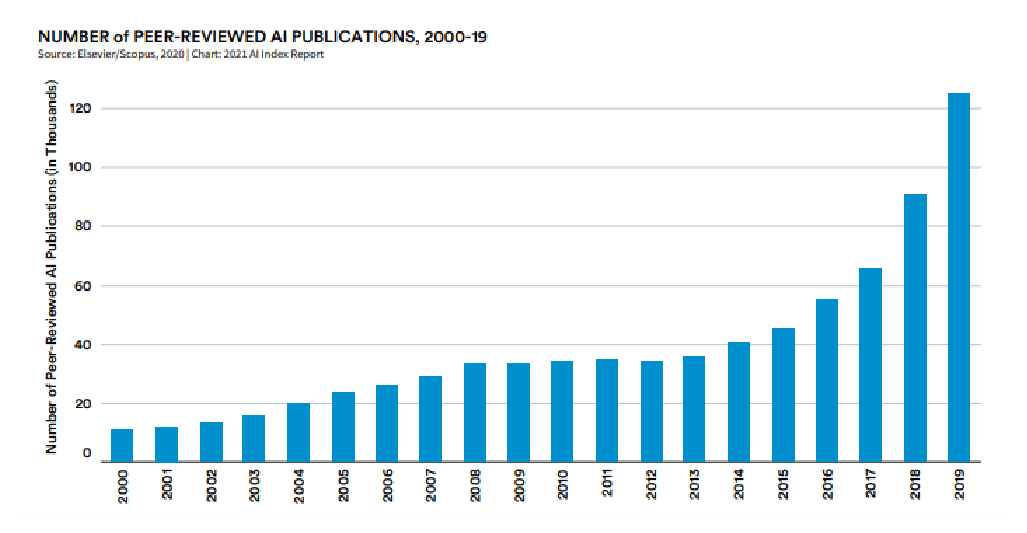
\includegraphics[scale=0.9]{images/chapter_1/AI_report.eps}}
\caption{Number of peer-reviewed AI publications, 2000-2019 \citep{zhang2021ai}}
\label{fig:Number of Peer-Reviewed AI Publications}
\end{figure}


\subsection{Review of opportunities for the manufacturing industry}

In this section, we present the result of a literature review we conducted to highlight some of the possible applications where machine learning could be applied in order to create value for manufacturing companies. This study should not, in any case, be considered as an exhaustive list of possibilities. Results are summarised in Table \ref{tab:ai_benefits}. 

\begin{table}
\label{tab:ai_benefits}
\caption{ML opportunities in manufacturing}
\begin{tabular}{|l|p{6cm}|p{4cm}|}
\hline
%
Domain &
  Benefits &
    Bibliography \\ \hline
Quality  &
  Decrease the product failure rate at the end of the production line. Optimise key performance index of the final product to meet customer needs. &
    \citep{lieber2013quality, li2018ensemble, chen2008neural, nagorny2017quality, haeussler1996quality} \\ \hline

Maintenance &
  Increase the availability of the production line by preventing the breakdown of equipment in advance. Predict the risk of malfunction of the production line and arrange proactive maintenance. &
    \citep{nguyen2019new, lee2017application, einabadi2019dynamic, li2017intelligent, liu2016prediction}\\ \hline
Fault Diagnosis &
  Prognostic diagnose of production line failure event. Identify the malfunction device of the production line. Predict the abnormal behaviours of machines and equipments. & \citep{toma2020bearing, wong2006modified, chen2014fault, malik2017artificial, arabaci2010automatic} \\ \hline
Scheduling  &
  Logistic management of the production line, which can maximise the throughput of the production line. Buffer control and product routing management. & \citep{morariu2020machine, woschank2020review, lolli2019machine, zhang2019review, gomes2016developing} \\ \hline
\end{tabular}
\end{table}


\section{Industrial domain: extrusion blow-moulding} \label{Industrial domain: extrusion blow-moulding}

Our industrial process, extrusion blow-moulding, isused to form hollow thermoplastic objects (especially bottles and containers). The process takes a thin-walled tube called a \textit{parison} that has been formed by extrusion, entraps it between two halves of a larger diameter mould, and then expands it by blowing air into the tube, forcing the parison out against the mould. The outside of the thin-walled part takes then the shape of the inside of the mould \citep{poli2001design}.

\begin{figure}
\centerline{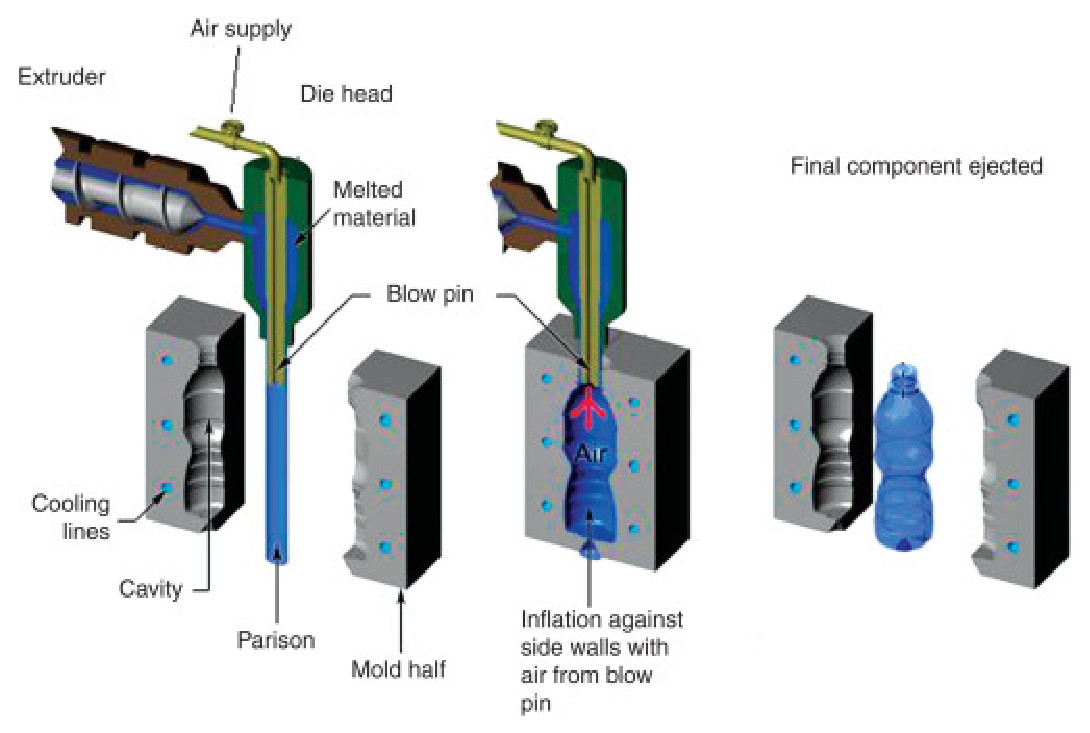
\includegraphics[scale=0.75]{images/chapter_1/extrusion_blow_molding.eps}}
\caption{Extrusion blow-moulding \citep{goodship2015design}}
\label{fig:Extrusion Blow-moulding}
\end{figure}

As the name suggests, extrusion blow-moulding is composed of two sub-processes: extrusion and blow-moulding.

\begin{itemize}
    \item \textit{Extrusion:} extrusion is a continuous-flow process where a plastic material feedstock is fed through a hopper onto a feeding transfer screw. The thermal energy provided by the heating clamps as well as the mechanical energy provided by the screw rotation allows the melting of the plastic material.The melted material is then pushed into an extrusion head and the die gap will typically create a tubular extruded cross-section, round or oval depending upon the final shape of the finished blow moulded part.
    The die gap is the distance between the inner mandrel and the outer bushing. The gap can be varied during the extrusion, due to the tapered nature of the die, by moving either the mandrel or the bushing in a vertical direction. The process of variable die gap extrusion is referred to as parison programming and is utilised to manipulate the thickness distribution in the final part \citep{diraddo1993profile}.
    \item \textit{Blow-moulding:} Unlike extrusion, blow-moulding is a discontinuous-flow process. In extrusion blow moulding, the parison is vertically suspended in the air during which time two mould halves enclose it by the action of a pneumatic or hydraulic mechanism. Internally applied air pressure causes the parison to inflate and take the shape of the inner parts of the moulds. Once the blow operation is completed and the part has been cooled down suitably for ejection, the mould opens and the part is ejected, allowing the parison to be extruded through the mould for the next cycle. 
\end{itemize}

Each phase has parameters that influence the subsequent phases and, ultimately, the characteristics of the finished product. The multiple phases mean that the number of parameters that can be adjusted on the process is fairly high. It is possible to fine-tune temperatures, screw speeds and throughputs for the extrusion, as well as the  pressure curves, moulds opening and closing times for the blow-moulding phase. In addition, the extrusion blow-moulding process has a certain dynamic: it takes a certain amount of time for the adjustment of one of the process parameters to have an effect on the products. This dynamic is mainly due to the thermal inertia of the solid tooling.
One of the most critical part of the process is the parison formation. In fact, the dimensions of the blow moulded article are directly related to the dimension and thickness of the parison. Furthermore, the thermo-mechanical history of the material during the parison formation stage and the resulting weight and diameter distribution of the parison have a great influence on the characteristics of the subsequent inflation and cooling stages. The shape and the dimensions of the parison are the result of complex interactions between the molten polymer and the thermo-mechanical conditions that influence the melt after it leaves the extruder die. Parison formation is affected by two phenomena knows as \textit{swell} and \textit{sag}. Parison swell, occurring both in diameter and thickness, is due to the nonlinear viscoelastic deformation of the polymer melt in the extrusion die. Sag is caused by gravitational forces that act on the suspended parison \citep{huang2002prediction}.

There are many variations of this process including equipment made to extrude multiple parisons simultaneously, equipment that can extrude multiple layers within the same parison, equipment with rotary capability that will hold several moulds and can provide a continuous nonstop process. Moreover, the extrusion blow-moulding process can be split into two subcategories: intermittent extrusion blow moulding and continuous extrusion blow moulding. With intermittent extrusion blow moulding, the extruder fills a reservoir with plastic. Once the the reservoir has been filled, a plunger is activated and pushes the material from the reservoir through the extrusion head. On the other hand, in continuous blow-moulding, the plastic is extruded permanently in a continuous manner while the machine runs.

In this thesis project we have been studying a continuous extrusion blow-moulding process, whose finished products are obtained from the overlay of multiple plastic layers. This particular type of blow-moulding process is known as \textit{co-extrusion}. Co-extrusion was born out of the need of reduce the permeability of fuel tanks. The steps for producing a multi-layer plastic product are the same as those used by the traditional single layer process, except for the number of extruders involved in the manufacturing process. Up to six extruders can be used simultaneously to melt different plastic materials. The goal is to create a multi-layer tank with the use of different materials, as shown in Figure \ref{fig:Co-extrusion Process}.

\begin{figure}
\centerline{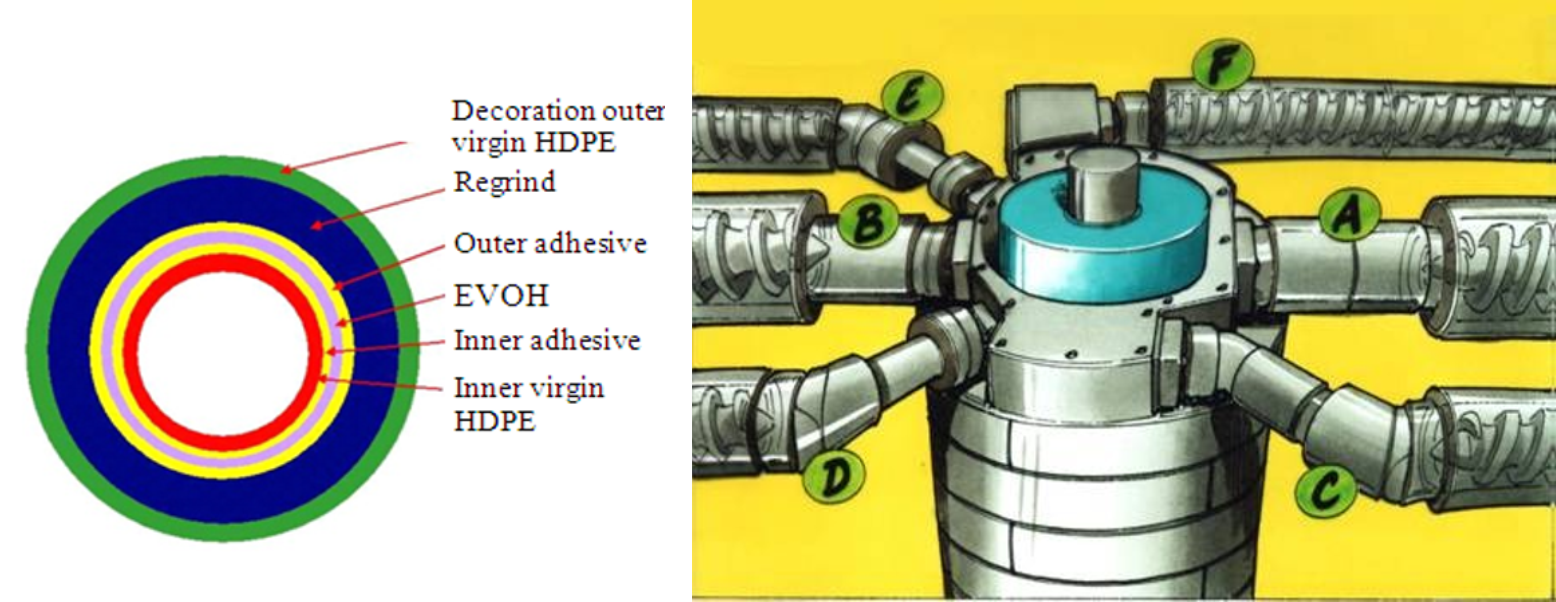
\includegraphics[scale=0.55]{images/chapter_1/coextrusion.png}}
\caption{Co-extrusion process}
\label{fig:Co-extrusion Process}
\end{figure}

The extrusion blow-molding process taken into account all along this research study is used to produce different tank models. In fact, by simply changing the moulds, it is possible to manufacture tanks with various shapes and sizes. The ratio between the separate plastic layers, as well as the material throughput, need to be adjusted accordingly to take into account the different size or shape of each tank model. This makes the extrusion blow-molding a flexible process which allows for rapid responses to costumers requests. The fuel tanks are usually manufactured in production campaigns of a few days, also known as batches.

The extrusion blow-moulding constitutes one of the various stages necessary to produce finished part. The stages needed to manufacture a finished part may vary depending on the type of product. For instance, a fuel tank container, a plastic bottle or a plastic bumper may require different post-production processes. Further information on how a fuel tank is produced are available in Appendix \ref{Full production process}. As far as our thesis work is concerned, we will only focus on the extrusion blow-moulding stage.

\subsection{The key parameters of the extrusion blow-moulding} \label{The key parameters of the Extrusion Blow-moulding}

Extrusion blow-moulding requires the fine-tuning of multiples adjustable parameters to reach the conditions for producing the final part. One of the most critical process parameter involving the extrusion sub-process is the material throughput. Controlling the amount of material passing through each extruder is crucial for the following reasons:  
%
\begin{itemize}
    \item It affects the cycle time. The throughput affects the ejection rate of the parison and therefore the cycle time. A cycle time reduction results in an higher manufacturing rate.
    \item The throughput ratios among the different 6 extruders should be controlled to ensure the correct amount of material on each of the 6 layers composing the tank thickness.
\end{itemize}
%
The throughput depends mainly on the rotation speed of the extruder and slightly on the extruder temperature. The temperature of the extruder affects the melting of the plastic material and the material viscosity may change. Depending on the material viscosity the throughput may change given the same extruder speed. For what has been said so far, controlling the temperature of the extruder along the screw length is mandatory to ensure constant and repeatable melting condition and therefore ensure a constant throughput. Another key parameter is the opening of the die gap of the \textit{head} of the machine. By controlling the opening of the gap during the cycle time we are able to distribute more or less material along the parison length. This operation is important to ensure to put enough material in parison zones that are most stretched during the blowing phase. Of course, the parison length plays a key role in ensuring that the material distribution is well positioned relatively to the mould position. Unfortunately, in the production process in question, there is no control system for measuring the parison length. In continuous extrusion blow-moulding, the cycle time triggers the blowing cycle. With regard to the blow-moulding sub-process, the most critical parameters are the blowing pressure, or better the blowing pressures, since there exist 4 different air blowing circuits, the cooling water temperature and throughput. The blowing pressure ensures the parison to inflate and take the shape of the inner parts of the moulds. Without enough air pressure the plastic material does not adhere to the mould surfaces, preventing a correct material cooling. In the same way, the amount of water passing through the cooling circuit, as well as its temperature, affect the cooling capacities of the moulds. The following table (Table \ref{tab:key_parameters}) summarises the key parameters of an extrusion blow-moulding process that were identified together with process experts.

\begin{landscape}
\begin{table}[]
\caption{Blow-moulding key
parameters}
\label{tab:key_parameters}
\begin{small}
\begin{tabular}{@{}llll@{}}
\toprule
\multicolumn{4}{c}{\textbf{Extrusion}} \\
\midrule
\textbf{Parameter}                     & \textbf{Range}   & \textbf{Description}                                    & \textbf{Dependencies} \\ 
\midrule
Speed$^*$  (in RPM)                               & [0, 90]       & Rotation speed of the screw                               &              \\ 
Throughput$^*$ (in Kg/h)                              & [0, 400]      & Material throughput in screw                 &  Speed, temperatures            \\ 
Melt pressure$^*$ (in \% of motor nominal torque)    & [0, 100]      & Pressure at the end of the screw                 & Speed             \\
Feeding temperature$^*$ (in °C)                               & [0, 100]      & Temperature at the entrance      &              \\
Melt temperature$^*$  (in °C)                                & [0, 250]      & Temperature at the end          &    Feed. temperature, pressure          \\
Cycle time   (in s)                                 & [60, 120]     & Tank production cycle time                                &              \\
Parison profile  (in \% of die gap opening)         &               &                                                &  Cycle time            \\
Parison length (in mm)                                & [0, 3000]     & Length during extrusion     &   Parison profile, cycle time    \\ 
\midrule
\multicolumn{4}{c}{\textbf{Blow-moulding}} \\
\midrule
\textbf{Parameter}                     & \textbf{Range}   & \textbf{Description}    & \textbf{Dependencies} \\ 
\midrule
Blowing pressure$^{**}$ (in bar)      &  [0, X]              & Blowing pressure inside moulds                                               &              \\
Cooling water temperature (in °C)     &  [5, 30]               & Temperature of cooling water (moulds)                                               &               \\
Cooling water throughput (in Kg/h)    &    []               & Throughput of the cooling water (moulds)                                               &              \\ 
\bottomrule
\end{tabular}
\end{small}

\footnotesize{%
\noindent
$^*$ For each extruder \\
\noindent
$^{**}$ There exist 4 different blowing circuits}\\
\end{table}
\end{landscape}

\subsection{The key quality characteristics of a blow-moulded fuel tank} \label{The key quality characteristics of a blow-moulded fuel tank}

Quality control is generally expressed as  the verification of the conformity of the process and the product/service to the requirements of its quality standard. The ISO 9000 standard defines quality control as ``a part of quality management focused on fulfilling quality requirements'' \citep{iso9000}. In our context, the requirements are defined by the customers, and measurements on the product and compared with the customer requirements, if the measurements meet the customer specifications, the part can be sent to the customer, otherwise the part must be rejected. In blow-moulded parts, , the distribution of the material over the entire surface of the part surface plays a key role in ensuring that the finished product meets customer specifications. In the extrusion blow-moulding process, we are mostly interested in the dimensional/geometric characteristics. In fact, the main purpose of the quality control of the blow-moulded part is to asses the integrity of the plastic shell. The thickness of the tank over the whole surface must be sufficient to ensure the robustness of the part and therefore its safety, while avoiding unnecessary excess weight on the finished product. Measuring the thickness of a hollow blow-moulded part is difficult as there is no access to the inner surface. Moreover, the thickness is relatively small, with value ranging from $3$ to $8$ millimetres. This requires an indirect measurement with an accuracy of at least $0.1$ millimetres.

\paragraph{Background in thickness measurement}

Traditional methods to measure the thickness of hollow parts rely on ultrasonic instruments that provide satisfactory results while avoiding the destruction of parts. The principle of \textit{Ultrasonic Thickness Measurement} (UTM) is to measure the time needed for the ultrasonic wave to traverse the material. Some of the advantages of UTM over other nondestructive methods are:
\begin{itemize}
    \item the possibility to measure parts with just one accessible surface,
    \item the suitability to industrial conditions,
    \item its sensitivity and accuracy.
\end{itemize}
 
These methods are extremely accurate for sample quality control, but they present a major drawback: they cannot be used for online measurement. The measurement of a large number of points, which is necessary to estimate the distribution of the material over the entire surface, is time-consuming and cannot be done online in production. Hence, the quality control of wall thickness is only carried using a sampling approach. Recently, new technologies involving the use of terahertz waves have been developed to accurately measure the thickness of materials without any contact with the material itself. These methods have proven to be extremely powerful for measuring the thickness of automobile paint \citep{su2014terahertz,krimi2016highly}, or pharmaceutical tablets \citep{may2011terahertz}. Of all the methods found in the literature, terahertz-based systems seem to be the only ones that can be used to perform real-time thickness measurement, but in order to use them in real-time, the measurement sensor must be installed on a robot, or collaborative robot, which can significantly affect the price of the complete measurement solution.

Another well-known technique for measuring thickness of parts is \textit{Computed Tomography} (CT). Typical areas of use for CT in industry are in the detection of flaws such as voids and cracks, and particle analysis in materials. In metrology, CT allows measurements of the external as well as the internal geometry of complex parts. As stated by \citet{de2014industrial}, CT is particularly suitable to investigate moulded polymer parts, thanks to the good penetrability of X-rays in this material. Even if CT-based techniques are extremely powerful, they require laboratory conditions and  do not lend themselves well to real-time thickness control. Moreover, this equipment may be very expensive, questioning its profitability.
%
Eddy current testing, widely applied for the non-destructive thickness measurement of metallic parts \citep{cheng2017thickness,mao2016thickness,wang2015noncontact,yin2007thickness}  is also non-destructive, but cannot be used as polymers composing the blow-moulded part are not conductive.

In the last decades,\textit{thermal imaging}, a non-contact technology capable of measuring large surfaces in a single shot, has been studied as a possible method to infer the thickness of a solid element \citep{sun2003method,sun2006analysis,choi2008quantitative,benitez2008definition,zeng2012absolute,li2018thickness,he2013eddy}. Among the most widely used thermal imaging approaches we can mention: \textit{pulsed thermography} in which a brief controlled thermal stimulation pulse is applied on the tested piece, \textit{step heating thermography}, in which a continuous, uniform heat flow is applied for a long period, and \textit{lockin thermography}, in which a periodic heat input is used. The main idea behind these approaches is to transfer energy to the test piece and to monitor its surface temperature evolution over time. In flash thermal imaging, for example, some flash lamps provide the thermal impulse, and the infrared camera monitors the surface-temperature decay on the heated surface. On the other hand, step-heating thermal imaging is using a long pulse of low intensity heat stimulation. Unlike pulsed thermal imaging, step-heating technology monitors the temperature raise over time while the heat energy is transferred to the test piece. The approach of monitoring the surface-temperature may also be applied without actively providing heat to the test part, especially for parts that are hot after the manufacturing process. The proposition of thermal imaging to measure the thickness of the tank is one of the major contributions of this research work and the proposed approach will be presented in detail in Chapter~\ref{Thickness inference using thermal imaging}.

Due to the impossibility of measuring the thickness of all parts produced, in practice, weight is often measured as an alternative. The weight is an indicator of how much material is composing the part and allows for an overall control of the quality of the part. The weight has a lower boundary to ensure that sufficient material is composing the tank and an upper boundary to avoid unnecessary weight of the finished product. Unlike the thickness, which has to be measured in several areas of the tank and cannot be carried out online for all the parts, the weight requires a simple weight scale, placed in the area where the blow-moulded part is discharged. 

Another quality issue that may occur is the fuel tank contamination. If the extrusion blow-moulding machine screws are not properly emptied following the so called purge procedures, or cycles, some material can remain attached to the screws and can solidify. This may cause the presence of unwanted burned material in the manufactured fuel tank, which generates a visual non-conformity of the part, and which can lead to tank permeability problems. The contamination problem identification completely relies on human visual inspection.

In order to produce a complete fuel system (see Appendix \ref{Plastic Omnium}), other manufacturing process are required after the extrusion blow-moulding (see Appendix \ref{Full production process}). Operations such as components welding or the assembly of pieces require further quality checks. The deepening of any quality control that does not directly concern the extrusion blow-moulding is out of the scope of this research work.  
%
\begin{table}[]
\caption{Quality indicators of a blow-moulded fuel tank }
\label{tab:quality_inidcators}
\begin{tabular}{@{}lllp{6cm}@{}}
\toprule
\textbf{Indicator} & \textbf{Unit} & \textbf{Value range} & \textbf{Description}                                                 \\ 
\midrule
Global Thickness           & mm                        & {[}3, 8{]}           & Thickness of the part measured at several critical points \\ 
Weight & Kg & {[}6, 14{]} & Total weight \\ 
\bottomrule
\end{tabular}
\end{table}
%
Table \ref{tab:quality_inidcators} summarises the two quality characteristics of a blow-moulded part we are interested in, and which must be monitored to ensure that the parts produced comply with customer requirements. However, in Chapter \ref{From Corrective to Predictive Process Control}, we will present an initiative which aims to partially reduce the contamination problems.

\section{Quality control and process monitoring in the extrusion blow-moulding process: a state-of-the-art} \label{state-of-the-art}

A literature review was carried out to identify previous work aimed at improving the overall quality of parts produced by a blow-moulding process. The literature review was carried out using three different databases: \textit{Scopus}, \textit{Google Scholar} and \textit{Crossref}. Subsequently, a screening exercise was carried out to select only the most interesting articles relevant to our scientific problem. Only about ten articles were identified as potentially interesting and strictly related to our research work. Figure \ref{fig:wordcloud} highlights the recurring words in the title and abstract of the retained articles. 

\begin{figure}
\centerline{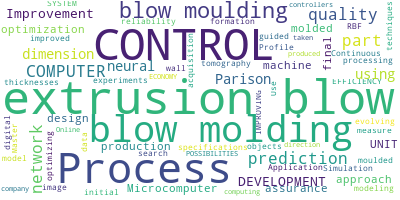
\includegraphics[scale=1]{images/chapter_2/wordcloud.png}}
\caption{Most recurrent words in article titles}
\label{fig:wordcloud}
\end{figure}

Two main strategies have been developed to improve the quality of the blow-moulded parts: \textit{expertise-based} and the \textit{data-driven } approaches. In the remaining part of the current section, we will investigate these two approaches proposed in the literature and we will discuss the possibility of using these methods in our industrial context. 


\subsection{Expertise-Based approaches} \label{Expertise-based approaches}

Expertise-based approaches make use of physics and simulation to model the manufacturing process and to fine tune process parameters given the simulated final part characteristics. Different strategies have been used to model the whole process that is the parison extrusion, clamping, inflation and cooling. \citet{lee1996prediction} used a finite element model of thin film to simulate blow moulding processes, and applied the feasible direction method to minimise the parison volume at the constraints of part thickness. The proposed parison design simulation is composed of the following stages. The finite element model predicts the thickness of the blow-moulded part from a given parison profile or preform. The resulting thickness distribution of the part is submitted to the optimisation model to generate a new parison profile. The new preform design is compared with the old one. If there is any improvement, the new preform design is again passed to the finite element model, and the loop is repeated until no further design improvement can be achieved. Author showed that the presented approach makes the optimisation algorithm more efficient and reduces the computational requirement drastically. 

Other expertise-based methods rely on iterative fine-tuning loop involving the prediction of the final part characteristics, such as the weight or the thickness. Two approaches, with regard to material behaviour during inflation, have been applied for the prediction. The first method assumes that the polymer melt behaves as a viscous or a viscoelastic fluid, whereas the second method assumes that the melt behaves as an elastic solid. The assumption that the parison behaves as a viscous or a viscoelastic fluid results in a very complex computational formulation. \citet{poslinski1990nonisothermal} treats the parison as a Newtonian fluid subject to a non-isothermal inflation. Parison position and cooling during the inflation are predicted as a function of time. Some experimental final part thickness distributions are obtained and compared to simulation results for a simple mould geometry and a constant initial thickness preform. Also, the inherent elastic nature of the polymer melt is not considered, since the formulation assumes a Newtonian fluid. \cite{ryan1982dynamics} and \citet{khayat1992inflation} assume a viseoelastic behaviour of the polymer melt. The inflation is modelled as a dynamic process, predicting the parison inflation as a function of time. A free inflation was considered; attempts with confined inflation, that is, employing a mould geometry, have not been handled to date. 
The approaches discussed by \citet{poslinski1990nonisothermal,ryan1982dynamics,khayat1992inflation} are interesting but make very strong assumptions or deal with very particular cases.

\citet{attar2008manufacturing} proposed an approach to assist the development phase of a new product and to optimise the weight of the part and its thickness distribution. Firstly, simulation of the extrusion blow moulding process and preliminary experimental trials were performed concurrently to assist in the development of the part. Once the numerical modelling of the part is done, improvement of the production process is performed based upon the desired objective function, i.e., a uniform part thickness distribution and/or minimal part weight. The optimisation is performed in two sequential steps, weight optimisation then thickness optimisation, by the systematic manipulation of the operating conditions, such as the parison dimensions. A process modelling methodology was employed to demonstrate the reduction in the part development time using the new model-based approach (Figure \ref{fig:workflow_development_process_optimisation}).
\begin{figure}
\centerline{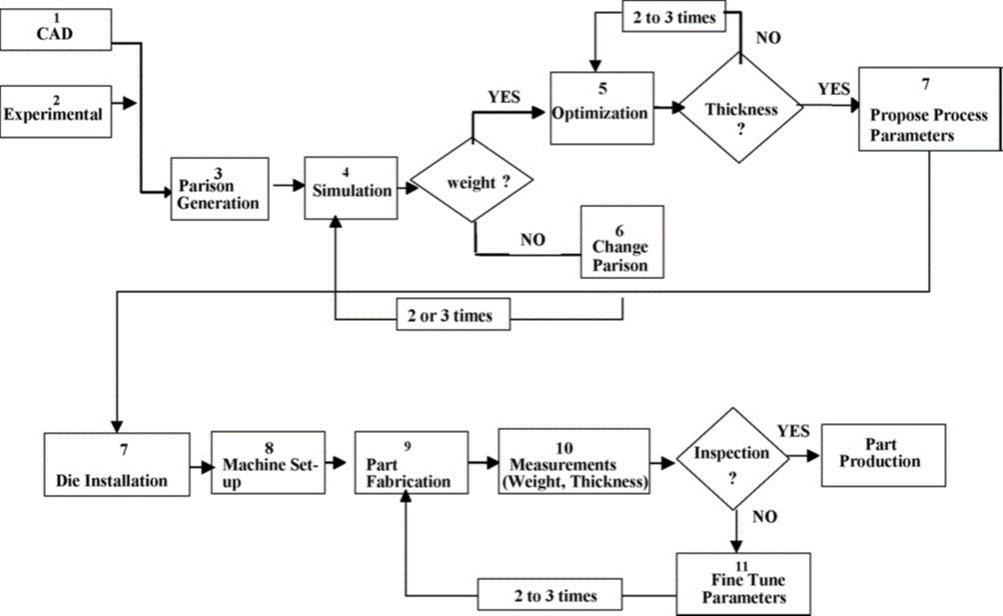
\includegraphics[scale=0.6]{images/chapter_2/optimisation_flow.png}}
\caption{Workflow for development process optimisation \citep{attar2008manufacturing}}
\label{fig:workflow_development_process_optimisation}
\end{figure}
It is a trial and error process, which is time-consuming and produces a lot of material scrap. On the other hand, the concurrent process optimises parameters virtually, and therefore, eliminates scrap, machine downtime and the need for experimental optimisation. The results demonstrate that there is a significant reduction in span time and in effort, since much of the delay and rework is eliminated using the simulation-based development process.


\subsection{Data-Driven approaches} \label{Data-driven approaches}

As the production process is complicated to be modelled physically, most of the work carried out previously makes use of data-driven methods to understand what process parameters affect the most the quality of the blow-moulded parts. The patterns discovered within data allow a subsequent optimisation of the process parameters.

\citet{diraddo1993line} have employed an entirely different methodology as a forward predictor of the inflation process. Neural networks are used for the on-line prediction of the final part thickness distribution from the initial process conditions. The fully connected neural network inputs include the initial parison thickness and temperature profiles, the bottle mould geometry and a rheological parameter representative of the raw material. The output data corresponds to 71-dimensional vector representing the thickness of 71 sampling points over the bottle length. The bottle thickness profile was measured by cutting the bottle into segments and measuring each with a hand micrometer. The neural network (see Section \ref{Neural network}) is trained by employing a gradient descent optimisation regression approach and mapping a broad range of output and input data. Once trained, the neural network predicts outputs based on new inputs. Authors claimed that the proposed data-driven method has several advantages over simulation-based methods. On first principles include faster response and the network’s ability to update a model to account for process shifts. Neural networks do not allow for an understanding of process fundamentals, they require a great deal of experimental data for the training procedure and problems can arise with extrapolation beyond the range defined by the experimental data. Therefore, the methodology is better suited for on-line applications, where fast response and following of process shifts is crucial. The same authors have employed neural networks for the modelling of the process with the inverse formulation \citep{diraddo1993modeling}. Compared to the previous approach, they tried to predict the initial parison thickness given the thickness of the final part. It would be valuable to determine the process conditions given the specified final part thickness distribution. The proposed approach was, in most cases, able to predict the constant thickness parison profile required for the specified part thickness distribution.   

\citet{ramana2013data} propose another use of data mining techniques to identify the factors that significantly affect quality, modelling relationships between input attributes and target attribute (yield, quality, performance index, etc) and predicting quality levels of given input attributes. A clustering analysis is first applied on process data to partition the population in different groups. By comparing these groups with data labels, they observe that rejected parts are classified in different groups than parts that meet the customer's specifications. Naive Bayes and decision tree are then applied with the main purpose of classifying the quality of the parts given the input parameters. The process parameters used as input data are: the process cycle time, the extruder temperatures in different zones, the extrusion die temperature, the expulsion time, the parison length, the parison shape, the blowing pressures and the inflation time. Naive Bayes and clustering models were found to have better accuracy compared to decision trees. The Authors claim that the model deployment has led to a general improvement in the quality of the parts. Unfortunately, the scientific paper does not provide any additional information on how the model was deployed. 

\subsection{Discussion} \label{Discussion}

Two different approaches have been proposed in the  scientific literature regarding quality optimisation in extrusion blow-moulding processes: expertise-based and data-driven approaches. Both methods try to predict the quality of the final part given the process conditions with the main purpose of fine-tuning the manufacturing process; they have relative advantages and disadvantages. Expertise-based approaches need strong assumptions or simplification to account for the overall process complexity. Data-Driven methods are faster and they can be used online. On the other hand, they require a great deal of experimental data for fitting their models and problems can arise with extrapolation beyond the range explored by the experimental data. 

The literature also highlight other fundamental aspects:

\begin{itemize}
    \item Due to the complexity of the studied production process, most recent approaches to improving process control or the quality of manufactured parts use data-driven methods \citep{diraddo1993line, diraddo1993modeling, ramana2013data}.
    \item No articles where found on the process of multi-layers extrusion blow-moulding (Co-extrusion). The literature presented mainly focuses on plastic bottle or simple plastic containers which are commonly produced through mono-layer extrusion blow-moulding. For this reason, some of the proposed methods are not applicable to our production process. For instance, the approach of \citet{diraddo1993line} for evaluating the geometrical dimensions of a plastic bottle requires the measurements of the material throughput exiting the extrusion head as well as the rheological parameter representative of the raw material. For technical and economical reasons, this information is impossible to collect in our production process.
    \item Most of the presented research works have focused on the product development phases, with little attention paid to controlling the quality of the part in production. It would be interesting to identify in real-time those factors that can lead to a degradation of the product quality. This would allow a faster process adjustment and even greater reduction of the scrap rate.

\end{itemize}

Supported by the scientific literature, and taking into account technological advances in the domain of the data acquisition in the manufacturing environment, we claim that data-driven methods are the right tools to investigate the interactions between extrusion blow-moulding process data and the corresponding product quality data. We claim that this is particularly true in a co-extrusion production process, where there are six extrusion screws, extruding 6 different types of polymers with different physical-chemical properties. In our opinion, physically modelling the co-extrusion production process would be quite complicated as too many assumptions would have to be taken into account. The interest of using data-driven methods is also confirmed by the scientific literature of the last years involving quality improvement. Data-Driven methods for product quality control have been successfully applied in multiple industrial domains, from steel industry \citep{lieber2013quality,li2018ensemble} to plastic industry \citep{chen2008neural,nagorny2017quality,nagorny2018generative,haeussler1996quality,tellaeche2013machine,sharma2017taguchi} and to the semiconductor manufacturing processes \citep{melhem2016regression,lenz2013data,jiang2020novel}.

\section{Research objectives and methodology} \label{Research objectives and methodology}

Because manufacturing processes are becoming more and more complex, and the high level of requirement in the automotive industry regarding safety and environmental impacts, Plastic Omnium is continuously seeking for innovation throughout its different projects that allows the company to remain leader in its field. For Plastic Omnium, the Industry 4.0 paradigm can provide a new way of looking at performance, with a more precise and immediate vision (based on real-time indicators) of the entire production chain, but also the optimisation of production through the use of data-driven methods. An in-depth presentation of the activities of Plastic Omnium is available in Appendix \ref{Plastic Omnium}. We have identified four main pillars driving the Industry 4.0 revolution:

\begin{itemize}
    \item \textit{Smart factory} refers to the set of initiatives that enable for a real-time traceability of what is happening inside production plants. With a real-time system, raw materials, work in progress and finished products are bar coded and tracked throughout the manufacturing process. The digitisation of the data allows also for a better monitoring of the production performance.
    \item \textit{Digital industrialisation} refers to the set of initiatives that make use of Virtual Reality (VR) and digital twin models to reduce the deployments costs of new machine and to optimise the plant machine layout. Other initiatives aim to optimise the ergonomics. 
    \item \textit{Predictive quality}refers to the use of data-driven methods to reduce the rate of product rejection at the end of the production line. This topic also covers initiatives to improve quality control and reduce destructive testing for quality control purposes.  
    \item \textit{Predictive maintenance} refers to the use of data-driven methods that are meant to analyse equipment status and forecast when maintenance should be performed. Predictive maintenance aims to reduce the number and the duration of the unplanned down-times and to optimise the maintenance operations.
\end{itemize}
%
Figure \ref{fig:pillars} shows how these topics integrate within the research environment of Plastic Omnium.
%
\begin{figure}
\centerline{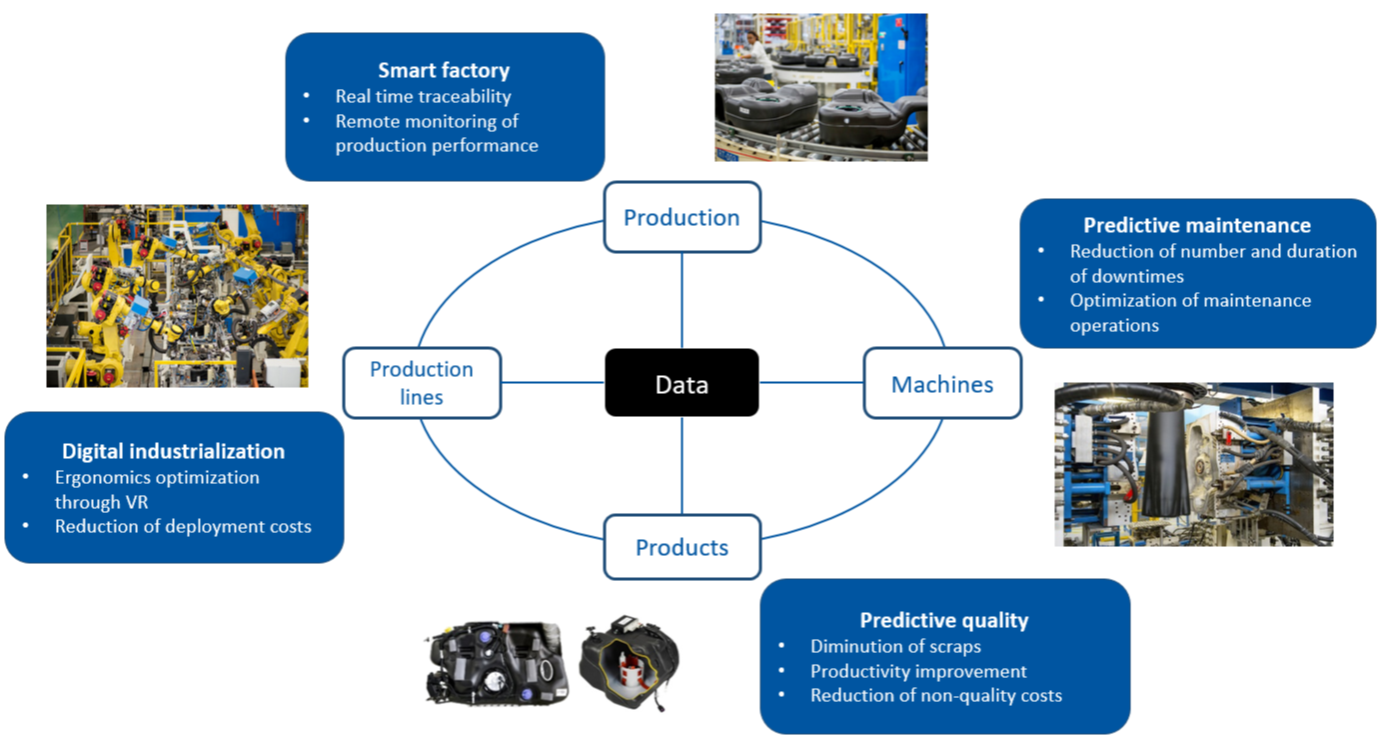
\includegraphics[scale=0.50]{images/chapter_1/Digitalisation_pillars.png}}
\caption{Industry 4.0 pillars for Plastic Omnium}
\label{fig:pillars}
\end{figure}
%
Among the different topics, this research work will focus on ``Predictive Quality'' topic. For an equipment manufacturer like Plastic Omnium Clean Energy Systems (CES), the “Cost of Non-Quality” (CNQ) is one of the key indicators most used to evaluate the production capacity and bad or ``scrap'' parts are not acceptable. Therefore, this research work aims at looking for the best way to use the data collected  on the machines and the corresponding product in order to propose a data driven approach inferring the quality of a product. The choice to use a data-driven approach is motivated by an ever-increasing availability of data within the manufacturing plants as well as from what has been said in the previous section (see Section \ref{state-of-the-art}). Using the data that is already available within the company will be an important part of the global study, because it will be the first input going into the developed monitoring system. In the case of Plastic Omnium CES, the data coming from the systems \textit{PES} (Production Execution System) and \textit{DASIP} (Data Acquisition for the Supervision of Industrial Process) will be important. The two systems allow for the traceability of the produced parts as well as a monitoring of the different events happening on the plant’s machines (for PES), and DASIP is monitoring key parameters of production processes. Other data sources will be investigated during this work.

This system will help detecting product non-conformities to plan the corrective actions accordingly. The expected benefits are:

\begin{itemize}
    \item the reduction of product non-conformities, 
    \item the overall quality control improvement,
    \item process improvement. In fact, product quality improvement requires working on the manufacturing process. This will help for a better comprehension of the extrusion blow-moulding process. 
\end{itemize}

To reach the final objective of reducing scraps and non-quality costs, a data-driven methodology will be proposed. The methodology is articulated around three principles consecutive stages, to best respond to the research objectives:
%
\begin{enumerate}
    \item Proposal of a general framework to deal with ``Predictive Quality'' topics, 
    \item Application of the proposed methodology to the studied industrial context,
    \item Proposal of a decision-making system. 
\end{enumerate}
%
Each of the four stages requires to overcome either some scientific or industrial issues or obstacles. In the scope of this thesis, we will only be able to work on the first two topics, although some elements concerning the last stage will be discussed in the conclusion of this research work. 

\paragraph{Proposal of a general framework to deal with ``Predictive Quality''}

During the first stage, we will leverage scientific literature to propose a general methodology to deal with all predictive quality topics. From an industrial point of view, this first stage requires identification of all necessary tools and methods needed to conduct a project from start to finish. 

\paragraph{Application of the proposed framework to the industrial context}

The application of the proposed framework to the industrial use case requires the critical data needed to answer our research question to be identified. Then, a machine learning algorithm will be applied to infer the quality of a part given the set of input parameters identified in the previous stage. From a scientific point of view, this stage will require to identify or build an efficient and robust machine learning algorithm able to model the transfer function which relates the input process data and the output quality data. 

\paragraph{Proposal of a decision-making system}

The last stage will involve the implementation of a decision-making system able to assess the quality of a produced part and, if necessary, to reject it. The system should be able to communicate with the systems already in place, such as the \textit{PES} system, to declare the part as non-compliant and to alert quality and production teams to trigger corrective actions. 

% Figure \ref{} ADD REF resumes the three stages of our methodology as well as the most important scientific and industrial issues which have to be overcome.

\section{Conclusion}

In this fist chapter, we have described the context of our research project. The French automotive company Plastic Omnium, leader in the production of automotive plastic components, aims to take advantage of fast growing amount of data available in manufacturing plants to improve quality of fuel tanks produced through extrusion blow-moulding manufacturing process. This complex manufacturing process is composed of two sub-processes: \textit{extrusion} and \textit{blow-moulding}. Extrusion is a continuous-flow process where a plastic material feedstock is fed through a hopper onto a feeding transfer screw. The thermal energy provided by the heating clamps as well as the mechanical energy provided by the screw rotation allow the melting of the plastic material. The die will typically create a tubular extruded cross-section, round or oval depending upon the final shape of the finished blow-moulded part. Unlike extrusion, blow-moulding is a discontinuous-flow process. In extrusion blow moulding, the parison is vertically suspended in the air during which time two mould halves enclose it by the action of a pneumatic or hydraulic mechanism. Internally applied air pressure causes the parison to inflate and take the shape of the inner parts of the moulds. The fuel tank produced through this manufacturing process must respect some dimensional and geometrical constraints to comply with customer specifications. The thickness of the tank over the whole surface must be sufficient to ensure robustness of the part and therefore its safety, while avoiding an excessive and unnecessary weight of the finished product. The scientific literature, involving quality control and process monitoring in the extrusion blow-moulding process, identifies two different ways of working on the topic of improving the quality of a blow-moulded parts. The first approach mainly relies on expertise and expert systems to optimise the manufacturing process. The second method makes use of data and data-driven methods to try to explain the variability of final part quality given the input manufacturing process parameters. The limitations of the approaches proposed in the literature, as well as the motivations that have oriented us towards the use of data-driven methods have been discussed. Finally, the main research objectives, as well as the research axes that will drive our research work, are presented. In the next Chapter, we will describe a general method to handle the predictive quality topics.   



% Chapter 2
\setcounter{mtc}{5}
\chapter{Background and related work: Quality control and machine Learning} \label{Background and related work: Quality control and machine Learning}
\minitoc

\section{Introduction}

Product and process failures anticipation have been the subject of multiple researches for decades. Since the introduction of the Statistical Process Control (SPC) in the early 1920s by Walter A. Shewart multiple methods have been proposed to monitor and control a process. From univariate Shewhart and  CUSUM \citep{woodall1985multivariate} \citep{crosier1988multivariate} control charts to multivariate methods such as Hotelling T², EMWA \citep{lowry1992multivariate} and Multi-way Principle Component Analysis (MPCA) \citep{nomikos1994monitoring}. These methods work well to identify unstable operating conditions but they have a limitation: the relationship between process parameters and product quality is not taken into account. These methods use only the information about the process operational behaviour and they describe how process measurements deviate from their average trajectories. As a consequence, some abnormality in process measurement may be irrelevant to the quality of the manufactured products. Recent advancements in machine Learning in the last few decades have opened up new research perspectives in the quality improvement domain. The first section of this chapter will be dedicated to the literature review related to the Blow-Molding process control and in particular to previous work involving the overall quality improvement. This literature review allows to define a starting position for our research work. In the second part of the chapter, we will review some notions about machine Learning that will provide the reader with the elements needed to understand the chapters 3, 4 and 5 of this PhD dissertation. 

\section{Quality control and Process Monitoring in the Extrusion Blow Molding process: a state-of-the-art} \label{}

Since we are interested in improving the overall quality of the part produced through the Extrusion Blow-Molding process, a first work of literature review has been done to identify previous works in this domain. The literature review have been carried out using three different databases: \textit{Scopus}, \textit{Google Scholar} and \textit{Crossref}.

The global research query used to find potential interesting articles is the following:

\begin{verbatim}
    ("extrusion blow molding"  OR  "extrusion blow-molding"  OR
    "extrusion blow-moulding"  OR  "extrusion blow moulding" )  
    AND   ( "process control"  OR  "process monitoring"  OR
    "quality control"  OR  "quality prediction"  OR  "anomaly detection" )
\end{verbatim}

Subsequently, a screening exercise was carried out to select only the most interesting articles relevant to our scientific problem. Figure \ref{fig:wordcloud} highlights the recurring words in the title and abstract of the retained articles. 

\begin{figure}
\centerline{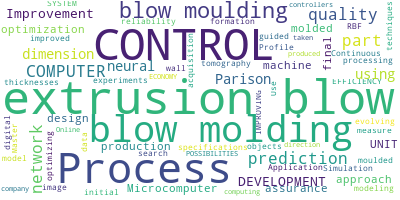
\includegraphics[scale=1]{images/chapter_2/wordcloud.png}}
\caption{Most recurrent words in article titles}
\label{fig:wordcloud}
\end{figure}

The bibliographical research work has highlighted two main strategies to improve the quality of the blow-molded parts:

\begin{itemize}
    \item Physics-based approaches: The first approach makes use of physics and simulation to model the manufacturing process and to fine tune process parameters given the simulated final part characteristics. 
    \item Data-driven approaches: As the production process is complicated to be modelled physically, most of the work carried out previously makes use of data-driven methods to understand what process parameters affect the most the quality of the blow-molded parts. The patterns discovered within data allow a subsequent optimisation of the process parameters.
\end{itemize}


In the remaining part of the current section, we will investigate the approaches proposed in the literature and we will discuss the possibility of using this methods in our industrial context. The following two subsections will provide more details about the two identified research strategies: physics-based approaches (\ref{Physics-based approaches}) and data-driven approaches (\ref{Data-driven approaches}). 

\subsection{Physics-based approaches} \label{Physics-based approaches}

Different strategies have been used to model the whole process that is the parison extrusion, clamping, inflation and cooling. \citep{lee1996prediction} used a finite element model of thin film to simulate blow molding processes, and applied the feasible direction method to minimise the parison volume at the constraints of part thickness. The proposed parison design simulation is composed of the following stages. The finite element model predicts the wall thickness of the blow-molded part from a given preform thickness. The resulting wall thickness distribution of the part is submitted to the optimisation model to generate a new preform thickness profile. The new preform design is compared with the old one. If there is any improvement, the new preform design is again passed to the finite element model, and the loop is repeated until no further design improvement can be achieved. Author showed that the presented approach makes the optimisation algorithm more efficient and reduces the computational requirement drastically. 

Others physics-based methods rely on iterative fine-tuning loop involving the prediction of the final part characteristics, such as the weight or the thickness. Two approaches, with regard to material behaviour during inflation, have been applied for the prediction. The first method assumes that the polymer melt behaves as a viscous or a viscoelastic fluid, whereas the second method assumes that the melt behaves as an elastic solid. The assumption that the parison behaves as a viscous or a viscoelastic fluid results in a very complex computational formulation. \citep{poslinski1990nonisothermal} treat the parison as a Newtonian fluid subject to a non-isothermal inflation. Parison position and cooling during the inflation are predicted as a function of time. Some experimental final part thickness distributions are obtained and compared to simulation results for a simple mould geometry and a constant initial thickness preform. Also, the inherent elastic nature of the polymer
melt is not considered, since the formulation assumes a Newtonian fluid. \cite{ryan1982dynamics} as well as \citep{khayat1992inflation} assume a viseoelastic behaviour of the polymer melt. The inflation is modelled as a dynamic process, predicting the parison inflation as a function of time. A free inflation was considered. Attempts with confined inflation, that is employing a mould geometry, have not been handled to date. 
The approaches discussed in \citep{poslinski1990nonisothermal}, \cite{ryan1982dynamics} \citep{khayat1992inflation} are interesting but make very strong assumptions or deal with very particular cases.

In 2008 \citep{attar2008manufacturing} proposed an approach to assist the development phase of a new product and to optimise the weight of the part and its thickness distribution. Firstly, simulation of the extrusion blow moulding process and preliminary experimental trials were performed concurrently to assist in the development of the part. Once the numerical modelling of the part was done, improvement of the production process was performed based upon the desired objective function, i.e., a uniform part thickness distribution and/or minimal part weight. The optimisation was performed in two sequential steps, weight optimisation then thickness optimisation, by the systematic manipulation of the operating conditions, such as the parison dimensions. A process modelling methodology was employed to demonstrate the reduction in the part development time using the new model-based approach (Figure \ref{fig:workflow_development_process_optimisation}).
\begin{figure}
\centerline{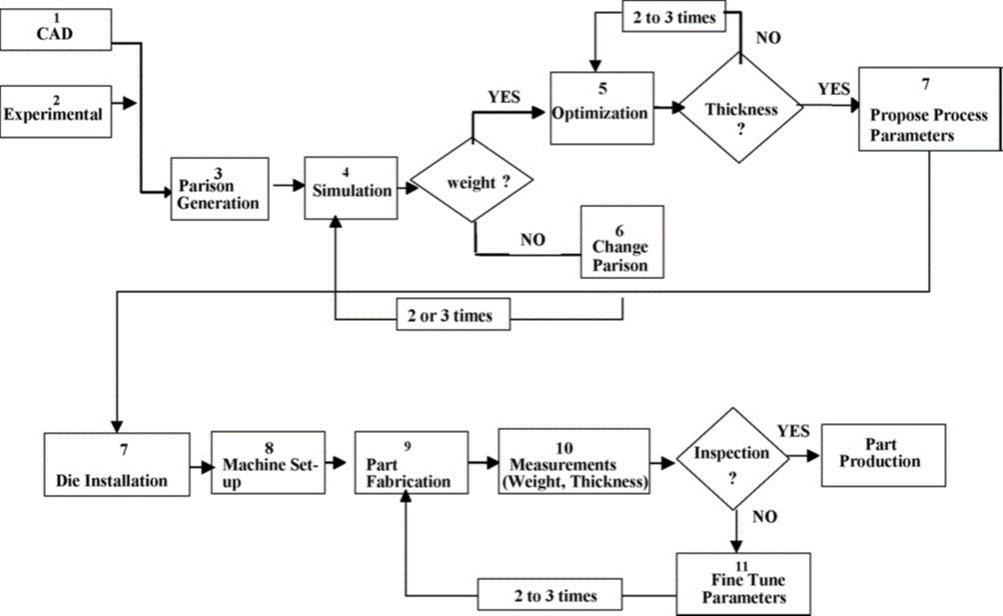
\includegraphics[scale=0.6]{images/chapter_2/optimisation_flow.png}}
\caption{Workflow for development process optimisation \citep{attar2008manufacturing}}
\label{fig:workflow_development_process_optimisation}
\end{figure}
It is a trial and error process, which is time-consuming and produces a lot of material scrap. On the other hand, the concurrent process optimises parameters virtually, and therefore, eliminates scrap, machine downtime and the need for experimental optimisation. The results demonstrate that there is a significant reduction in span time and in effort, since much of the delay and rework is eliminated using the simulation-based development process.


\subsection{Data-driven approaches} \label{Data-driven approaches}

\citep{diraddo1993line} have employed an entirely different methodology as a forward predictor of the inflation process. Neural networks are used for the on-line prediction of the final part thickness distribution from the initial process conditions. The Fully connected neural network inputs include the initial parison thickness and temperature profiles, the bottle mold geometry and a rheological parameter representative of the raw material. The neural network is trained by employing a gradient descent optimisation regression approach and mapping a broad range of output and input data. Once trained, the algorithm is capable of predicting outputs based on new inputs. Authors claimed that the proposed data-driven methods has several advantages over simulations based methods. On first principles include faster response and the network’s ability to update a model to account for process shifts. Neural networks do not allow for an understanding of process fundamentals, they require a great deal of experimental data for the training procedure and problems can arise with extrapolation beyond the range defined by the experimental
data. Therefore, the methodology is better suited for on-line applications, where fast response and following of process shifts is crucial. The same authors proposed in \citep{diraddo1993modeling} another have employed neural networks for the modelling of the process with the inverse formulation. Compared to the previous approach they tried to predict the initial parison thickness given the thickness of the final part. It would be valuable to determine the process conditions given the specified final part thickness distribution. The proposed approach was, in most cases, able to predict the constant thickness parison profile required for the specified part thickness distribution.   

Another interesting approach have been carried out by \citep{ramana2013data}. They propose to use data mining techniques to identify the factors that significantly affect quality, modeling relationships between input attributes and target attribute (yield, quality, performance index etc) and predicting quality levels of given input attributes. Clustering analysis have been initially applied on process data to split the entire population in different clusters. The cluster analysis made it possible to categorise the data into different families. By comparing the results of the cluster families analysis with the data labels, they prove that reject part are categorised in different clusters than parts conforming to customer specifications. Naive Bayes and Decision Tree has been then applied with the main purpose of classify the quality of the part given the input parameters. The process parameters used as input data are: the process cycle time, the extruder temperatures in different zones, the Extrusion Die temperature, the expulsion time, the parison length, the parison shape the blowing pressures as well as the inflation time. Naïve Bayes and clustering models were found to have better accuracy than Decision Trees in the evaluation performed by standard lift chart while predicting process parameter values that result in acceptable products. The knowledge driven and proactive decisions have been implemented in quickly setting process parameters and their range of values that resulted in increased output of high quality products and significantly reduced the scrap.

\subsection{Discussion} \label{Discussion}

The scientific literature pointed out previous works in the domain of Extrusion-Blow Molding process and quality optimisation. Two different approaches have been presented: physics-based and data-driven approaches. Both have advantages and disadvantages. Physics-based approaches need strong assumptions or simplification to account for the overall process complexity. Data-driven methods are faster and they can be used online. On the other hand, they require a great deal of experimental data for the training procedure and problems can arise with extrapolation beyond the range defined by the experimental data. Both methods try to predict the quality of the final part given the process conditions with the main purpose of fine-tuning the manufacturing process. 

This bibliographical research work has made it possible to highlight two other fundamental aspects:

\begin{itemize}
    \item Due to the complexity of the studied production process, most recent approaches to improve the quality of the manufactured parts or to improve the process control make use of data-driven methods.
    \item None of the articles considered deals with the process of multi-layers Extrusion Blow-Molding (Co-extrusion). Extrusion-Blow molding scientific literature mainly focus on plastic bottle or simple plastic containers which are commonly produced through mono-layer extrusion blow-molding process. For this reason, some of the proposed methods are not directly applicable to our production process. For instance, the approach presented by \citep{diraddo1993line} for evaluating the geometrical dimensions of a plastic bottle is really interesting. On the other hand, among the input process data used as predictors, they use the material throughput exiting the extrusion head as well as the rheological parameter representative of the raw material. This information is missing from the production process under consideration and any modification to the machine to retrieve the missing information would not be possible for technical and economical reasons.
    \item Previous research work deals mainly with the development phases of the products. Only a few of the literature works are concerned with improving the quality of the part in production. When the machine is properly set, the scrap rate is close to $0$. On the other hand, there are certain internal or external factors which can cause the production of non-conforming parts. It would be interesting to identify in real-time, or even prevent, these factors that can lead to a degradation of the product quality. This would allow a faster process adjustment and even greater reduction of the scrap rate.
\end{itemize}

 
Starting with the results obtained by \citep{diraddo1993line} and \citep{ramana2013data}, and with the advancement of machine Learning techniques in the last decade, we decided to move our attention towards data-driven methods. Supported by the scientific literature, and taking into account technological advances in the domain of the data acquisition in the manufacturing environment, we claim that data-driven methods are the right tools to investigate the interactions between Extrusion Blow-Molding process data and the corresponding product quality data. We claim that this is particularly true in a Co-extrusion production process, where there are six extrusion screws, extruding 6 different types of polymers with different physical-chemical properties. Physically modelling the production process would be quite complicated as too many assumptions would have to be taken into account. The interest of using data-driven methods is also confirmed by the scientific literature of the last years involving quality improvement. Data-driven methods for product quality control have been successfully applied in multiple domains, from steel industry \citep{lieber2013quality,li2018ensemble} to plastic industry \citep{chen2008neural,nagorny2017quality,haeussler1996quality,tellaeche2013machine,sharma2017taguchi} and to the semiconductor manufacturing processes \citep{melhem2016regression,lenz2013data,jiang2020novel}.

In the next section, some basics of machine Learning are presented with the aim of providing the reader with all the necessary elements to follow chapters 3, 4 and 5.

\section{Machine learning}

Machine learning is a field of computer science that aims to give computers the ability to learn and act without being explicitly programmed.  Traditionally, computer software is developed on the basis of a series of logical conditions constantly repeating. Instead of explicitly encoding knowledge by machine instructions, machine learning leverages data analysis, which involves building and fitting models, to allow machines to 
``learn'' from experience. Machine learning consists in building algorithms to improve the ability of machines to make predictions. Researchers and manufacturers have developed, over the years, a myriad of different kinds of Machine Learning (ML) models, or algorithms serving different situations and types of problems.

In this section we will review some concepts about machine learning in order to provide the reader with the basic elements to understand the following chapters of this PhD dissertation. Initially, some of the key concepts related to the machine learning such as difference between \textit{Supervised} and \textit{Unsupervised} learning is presented. Subsequently we will describe a few methods that have been applied all along the doctoral studies. This review is in no way intended to be exhaustive but wants to provide the necessary elements for understanding the approaches presented in chapters 3 and 4. For an exhaustive review of machine learning topics we suggest the following references: \citep{bishop2006pattern,friedman2017elements}. As regards deep learning, \citep{goodfellow2016deep} provides a comprehensive review of the most applied neural network based techniques. 


\subsection{Supervised learning}

The most widely used machine learning approach is the \textit{Supervised} one. Supervised learning is the task which involves learning a function from examples of its inputs and outputs. In supervised learning we look for a model that relates the response to the predictors, with the aim of accurately predicting the response for future observations (prediction) or better understanding the relationship between the response and the predictors (inference). In general, to solve a Supervised learning problem we look for a function that minimises an error (cost function). The cost function quantifies the overall error in prediction between the predictions of each training samples and the real value (or “grand-truth”) associated. The cost function changes depending on the problem that we want to solve: Regression or Classification.

\paragraph{Regression} \label{Regression}

Regression corresponds to a training objective where training data and their corresponding outcome, a set of numerical continuous variables, are known and available for training. More generally, suppose that we observe a quantitative response $Y$ and $p$ $(X_1,X_2,\ldots,X_p)$ different predictors. We assume that there is some relationship between $Y$ and $X = (X_1,X_2,\ldots,X_p)$, which can be written in the very general form: 

\begin{equation}
  Y=f(X) + \epsilon, \textnormal{ with } f:\mathbb{R}^{p} \rightarrow \mathbb{R}^{m}
  \enspace,
\end{equation}
where $f$ is some fixed but unknown function of $X_1,X_2,\ldots,X_p$, and $\epsilon$ is a random error term, which is independent of $X$ and has mean zero. The objective is to find an estimate of the function $\hat{f}$ that better approximates as well as possible the relationship between the response and predictors. For instance, in a manufacturing context, a regression model can be designed to predict the numerical value of some dimensional characteristic of a manufactured part, given a set of input process parameters.

\paragraph{Classification} \label{Classification}

Classification corresponds to a training objective where training data and their corresponding true outcome, called label or class, are known and available during the training phase. A machine learning model performing a classification is also called a \textit{classifier}. Its role is to infer on a label (good part/non compliant part, car/air-plane/truck, etc.) to apply to a given input data vector. The possible answers (i.e. labels or classes) are determined by the dataset given to the model during the training phase. All the possible labels need to be known during training. Given a set of $c$ different classes, an input vector composed of $p$ $(X_1,X_2,\ldots,X_p)$ different predictors, and an output vector of class probabilities $Y$, defined as follow:

\begin{equation}
    Y \in [0, 1]^{c} \textnormal{ with } \sum_{i=1}^{c} Y_{i} = 1
    \enspace,
\end{equation}
we look for the function $\hat{f}$ so that:

\begin{equation}
  Y=\hat{f}(X)+ \epsilon, \textnormal{ with } f:\mathbb{R}^{p} \rightarrow [0,1]^{c}
  \enspace,
\end{equation}

A compressed form is frequently found when there exist only two classes. This is also called \textit{binary classification}. In a manufacturing context, a classifier can be trained to recognise whether a part is compliant (OK), or not (NOK), to some quality specification.   

\paragraph{Time series classification/regression}

In some cases, we deal with several observations of the same variable over time. We define \textit{univariate time series} $T = [t_{1}, t_{2}, \dots, t_{K}]$ is an ordered set of real values. The length of $T$ is equal to the number of real values $K$. In the same way, we define an \textit{M}-dimensional Time Series, $T = [T_{1}, T_{2}, \dots, T_{M}]$ as a set of $M$ univariate time series with $T^{i} \in \mathbb{R}^{K}$. Given a dataset $D = \{(T_{1}, Y_{1}),(T_{2}, Y_{2}),\dots,(T_{N}, Y_{N})\}$ which corresponds to a collection of pairs $(T_{i}, Y_{i})$ where $T_i$ could either be a univariate or multivariate time series with $Y_{i}$ as its corresponding one-hot label vector. For a dataset containing $c$ classes, the one-hot label vector $Y_{i}$ is a vector of length $c$ where each element $j \in [1, c]$ is equal to $1$ is the class of $T_{i}$  is $j$ and \textit{0} otherwise. The task of \textit{Time series classification} consists of training a classifier on a dataset $D$ in order to map from the space of possible inputs to a probability distribution over the class variables values (labels) \citep{fawaz2019deep}. If we deal with a generic target variable $Y_{i}$, corresponding to a continous variable, the problem would take the name of \textit{Time series regression}. 


\subsubsection{Parametric models} \label{Parametric models}

Parametric models involve a two-step approach:
\begin{itemize}
    \item We make an assumption about the functional form of the function $f$.  
    \item Once the functional form is established, we need a procedure to estimate the model coefficients. 

\end{itemize}
	 
Among all parametric methods Linear Regression is the most common. The general linear function can be expressed with the following notation:

\begin{equation} \label{eq:linear_function}
    f(x)=\beta_0 + \beta_1X_1 + \beta_2X_2 + \ldots + \beta_pX_p
    \enspace,
\end{equation}
where $\beta_j$ is the generic $j$-th coefficient, associated with the $j$-th feature.
In Linear Regression, to estimate the model coefficients, we look for the hyper-plane that minimises the residual sum of squares:

\begin{equation}
    RSS = \sum_{i=1}^{n}(y_i -f(x_i))^2 = (Y - X\beta)^T(Y - X\beta)
    \enspace.
\end{equation}

Under the assumption that $X$ have full column rank, we can differentiate the equation with respect of $\beta$ to obtain the unique solution:

\begin{equation}
    \beta = (X^TX)^{-1}X^TY
    \enspace.
\end{equation}

One way to reduce the model variance is to apply a technique that constraints or regularises the coefficient estimates towards zero. The two best known methods are Ridge Regression \citep{hoerl1970ridge} and Lasso Regression \citep{tibshirani1996regression}. 

In Ridge Regression a penalty term is added to the loss function, this penalty term is also called $L2$ regularisation. The penalised residual sum of squares can be written as follows:

\begin{equation}
\begin{aligned}
 RSS_{Ridge}(\lambda) & = \sum_{i=1}^{n}(y_i -f(x_i))^2 + \lambda\sum_{j=1}^{p}\beta^{2}_{j} \\
& = \|Y - X\beta\|_2^2 + \lambda\|\beta\|_2^2
    \enspace,
\end{aligned}
\end{equation}
where $ \lambda \geq 0 $ is a complexity parameter that controls the amount of shrinkage towards zero and $||\beta||_2$ is the $L2$-norm (Euclidean norm). These parameters have to be determined separately, for example using cross-validation. The Ridge Regression coefficient estimation is given by:

\begin{equation}
    \beta_{Ridge} = (X^TX + \lambda I)^{-1}X^TY
    \enspace.
\end{equation}

Lasso Regression applies a similar shrinkage approach. In Lasso regression a penalty term ($L1$ regularisation), corresponding to an absolute value of magnitude, is applied to the residual sum of squares:

\begin{equation}
\begin{aligned}
 RSS_{Lasso}(\lambda) & = \sum_{i=1}^{n}(y_i -f(x_i))^2 + \lambda\sum_{j=1}^{p}|\beta_{j}| \\
& = \|Y - X\beta\|_2^2 + \lambda||\beta||_1
    \enspace,
\end{aligned}
\end{equation}
where $\lambda \geq 0 $ is a complexity parameter that can be estimated using cross-validation and $||\beta||_1$ is the $L1$-norm (Manhattan norm). As with Ridge Regression, the Lasso shrinks the coefficient estimates towards zero. However, the lasso penalty has the effect of forcing some of the coefficient estimates to be exactly equal to zero when $\lambda$ is sufficiently large. Lasso yields sparse models that are generally much easier to interpret than those produced by Ridge Regression. With Lasso, the features that are not related to the dependent variable are decreased towards zero so that this method is quite useful to do feature selection. Unlike Ridge Regression, however there is no closed form expression to solve the minimisation of the residual sum of squares. There are multiple algorithms for computing the entire path of solutions but their presentation is outside the scope of this paper. 

Linear, Lasso and Ridge Regression are parametric models suitable for solving Regression problems. When dealing with Classification, it is more suitable to use others approach. The most common parametric model to solve binary classification problems is \textit{Logistic Regression}. Logistic Regression is a transformation of a linear regression using the \textit{sigmoid} function: $sigmoid(x) = \frac{1}{1 + e^{-x}}$. The step from linear regression to logistic regression is kind of straightforward. In the linear regression model, we have modelled the relationship between outcome and features with a linear equation (\ref{eq:linear_function}). For classification, we prefer probabilities between $0$ and $1$, so we wrap the right side of the equation into the logistic function:

\begin{equation}
    P(Y=1) = \frac{1}{1 + e^{- (\beta_0 + \beta_1X_1 + \beta_2X_2 + \ldots + \beta_pX_p)} }
    \enspace.
\end{equation}
This forces the output to assume only values between 0 and 1.

\subsubsection{Tree-based methods} \label{Tree-based methods}

Tree based methods are simple and useful models for interpretation. These models use decision trees to determine which target value matches the observation. Decision trees split the feature space into multiple regions $R_j$ and than fit a simple model in each one. For every observation that falls into the region $R_j$ the prediction is simply the mean of the response values for the training observations in $R_j$. Another time, we look for the regions $R_j$ that minimise the residual sum of squares. Unfortunately, it is computationally infeasible to consider every possible partition of the feature space into j regions. In order to overcome this issue, we use a greedy top-down approach. The most widely used method is the CART algorithm \citep{breiman2017classification}. A CART Tree is a binary decision tree that is constructed by splitting a node into two child nodes repeatedly, beginning with the root node that contains the whole learning samples. The main idea is to grow the tree by choosing a split, among all possible splits, that maximise a defined splitting criterion. Usually the splitting criterion for regression trees is the mean squared error:

\begin{equation}
    MSE = \frac{1}{n}\sum_{i=1}^{n}(y_i -f(x_i))^2
    \enspace.
\end{equation}

Even though these model are quite good for interpretability, they are not competitive with others machine learning techniques in term of prediction. One possible way to improve the prediction capabilities is to use methods like Bagging \citep{breiman1996bagging}, Random Forest \citep{breiman2001random} and Gradient Boosting \citep{friedman2001greedy}.
With \textit{Bagging} (Boostrap Aggragation), several subsets of data are created from the training set and each of this subset is used to build a decision tree. By averaging the predictions of all the different decision trees we end up with more robust results and with the reduction of the variance of the estimated model. Given B different bootstrapped training set, the final prediction can be written as follow:

\begin{equation}
    f_{bagging}(x) = \frac{1}{B}\sum_{b=1}^Bf_b(x)
    \enspace,
\end{equation}
where $f_b(x)$ is the prediction on the $b$-th bootstrapped training set for a point $x$.
Random Forest can be seen as an extension of bagging. In addition to taking the random subset of samples, it takes a random subset of features. Once again, by averaging the results of the “Forest” generated by this method, we can obtain a more robust result compared to a single regression tree. 
Gradient Boosting is named after two different techniques: Gradient Descent and Boosting. In gradient boosting, the learning procedure consecutively fits new models to provide a more accurate estimate of the response variable. The principle idea behind this algorithm is to construct the new base-learners to be maximally correlated with the negative gradient of the loss function, associated with the whole ensemble. The loss functions applied can be arbitrary, but to give a better intuition, if the error function is the classic squared-error loss, the learning procedure would result in consecutive error-fitting \citep{natekin2013gradient}. 

\subsubsection{Support Vector Machines} \label{Support Vector Machines}

In 1992 Vapnik and coworkers \citep{boser1992training} proposed a supervised algorithm for classification that has since evolved into what are now known as \textit{Support Vector Machines} (SVMs): a class of algorithms for classification, regression and other applications that represent the current state of the art in the field.
The SVM methodology was originally conceived for binary classification problems. In a given feature space, SVM learning aims to construct a hyper-plane to best separate training data with different class labels. The hyper-plane is derived on the basis of a limited number of training instances, so-called support vectors, to maximise a margin on each side of the plane. When the samples are not linearly separable, it is possible to perform a $\Phi$ transformation, also called \textit{kernel trick} of the original data space, in order to find a space where the samples are linearly separable. The most commonly used non-linear kernels are polynomial and \textit{Radial Basis Function} (RBF) kernels.

\textit{Support vector regression} (SVR) \citep{drucker1997support}, an extension of the SVM algorithm, has been introduced for predicting numerical continuous values instead of classes. In SVR, instead of generating a hyper plane for class label prediction, a different function is derived on the basis of training data to predict numerical values. In analogy to SVM, SVR also projects training data with nonlinear structure–activity relationships in a given feature space into higher-dimensional space representations where a linear regression function may be derived.

\subsection{Unsupervised learning}

In numerous situations, collecting data and the corresponding expected output for training is too expensive or just very difficult to formalise or collect. When the objective is to design a model capable to group similar data points (i.e. clustering) without any clear predefined groups, the common approach is to explore \textit{Unsupervised Learning} (UL) methods and algorithms.

\paragraph{Clustering}

Clustering is an Unsupervised learning technique (i.e. a learning method where training data is fed into a model without the possibility to compare the output given by the model with a corresponding theoretically correct observation). Thus there is no correct answer, error or reward function, consequently the model does not rely on the availability of the domain’s experts. It is a common technique to perform knowledge discovery inside the data. Clustering focuses on finding patterns in the data to find different groups within the input data. This can be used to cluster (i.e. group) the data which are the most similar and apply later on a specific process to each of these groups.

\paragraph{Density Estimation}

Most UL objectives apart from clustering fit in a density estimation logic. One of the possible objectives with an UL could be to learn the structure of the input data distribution. Once done, a model is able to produce a new data point coming from the learned input data distribution, and thus very similar to the training data. 

This is in particular useful to create a generative model or a model able to detect any novelty, anomaly outlier data point. In many situations, there might be an interest to detect any deviation to the usual situation (e.g. IT security, dangerous situation detection, etc.). One of the common issue of these objectives is to be able to collect a representative dataset of both situation (i.e. normal and abnormal). Usually, abnormal events occur a lot less frequently, this inevitably results in an imbalanced data repartition, often by many orders of magnitude (e.g. 99.5\% normal data and 0.5\% abnormal data).


\subsection{Principal Component Analysis} \label{Principal Component Analysis}

\textit{Principal Component Analysis} \citep{pearson1901liii}\citep{hotelling1933analysis}, usually abbreviated to \textit{PCA}, is the reference dimensional reduction method that relies on a factorisation of the matrix representing the input data. Given a generic input data $X \in \mathbb{R}^{n \times p}$ the covariance matrix $C$ ca be computed as follow:

\begin{equation} \label{eq:covariance}
    C = cov(X) = \frac{1}{n - 1} \sum_{i=i}^{n} (X_{i} - \Bar{X})(X_{i} - \Bar{X})^{T}.
\end{equation}

The covariance matrix is symmetric and so it can be diagonalised:

\begin{equation}
    C = VLV^T
\end{equation}

where $V$ is the matrix of eigenevectors and $L$ is the diagonal matrix with eigenvalues. The eigenvecteurs of the covariance matrix $C$ take the name of \textit{Principal Components} of \textit{X}. The eigenvalues $\lambda_{k}$ can than be used to order the eigenvecteurs in ascending order of the variance of the data expressed by each eigenvector. By selecting $k$ Principal Components, with $k << n$ it is possible to account for most of the original dataset variability. Principal Component can be used either as a method of reducing the size of the input data space and as a Data exploratory tool. In fact, since the first Principal Components account for the most of the variability, in the majority of the cases it is possible to visualise most of the input data variability by projecting the input sample on the first 2-3 Principal Components. 


\section{Deep learning}

Deep Learning (DL) is a sub-field of ML focusing on deep neural network based architectures. DL models have become some of the top performing methods in the state-of-the-art outperforming traditional ML techniques for numerous applications and challenges. These last years have shown how deep Learning can be applied to solve multiple tasks and problems. Great improvements have been reached in multiple domains: from web searches to image recognition and classification through Convolutional neural networks to natural language preprocessing with Recurrent neural networks and \textit{Self-Attention} networks \citep{vaswani2017attention}. The democratisation of the different models through open-source software libraries, specialised chip-set and highly scalable computing platforms has pushed companies to integrate these tools within their own production facilities. The deep learning research is advancing very fast and new architectures are proposed every day. An exhaustive overview of DL is out of the scope of this research work but, in the following subsection we will introduce three different families of neural networks: Feed-forward neural network, Convolutional neural network and Recurrent neural network, as well as some specific architectures that we will applied in chapter 4.


\subsection{Neural network}

A neural network is a computing system made up of a number of simple, highly interconnected processing elements (units). Feed-forward neural networks learn to map a fixed-size input to a fixed-size output. To go from one layer to the next, the units compute a weighted sum of their inputs from the previous layer and pass the result through a non-linear function (activation function). For a generic hidden layer $H$ of a neural network the $j$-th unit compute the following operation:  

\begin{equation}
    h_j^H = \sigma(\sum_{i \in H-1}W_{ij}x_i)
    \enspace,
\end{equation}
where $W_{ij}$ is the weight on connection from unit $j$ and the $i$-th unit of the previous layer, and $\sigma$ is the activation function. Among all activation functions the most popular on these days are \textit{ReLu} (Rectified Linear Unit) \citep{Glorot2011DeepSR}, which is defined as follow:

\begin{equation}
    ReLu(x) = max(0,x)
    \enspace.
\end{equation}

Without the activation function the neural network would be a stacking of linear models and it would not be able to take into account non-linear connections between inputs and outputs. 
Units that are not in the input or output layer are conventionally called hidden units. The hidden layers can be seen as distorting the input in a non-linear way so that categories become linearly separable by the last layer \citep{DBLP:journals/nature/LeCunBH15}. During the training phase we compute an objective function that measures the error (or distance) between the output scores and the desired pattern of scores. The back-propagation algorithm uses the derivative chain rule to calculate the gradient of an objective function with respects to the weights of a multilayer stack of units. In other words, the gradient of the objective function with respect to the inputs can be computed by working backwards from the gradient calculated with the respect of the output. The gradient, for each weight, indicates by what amount the error would increase or decrease if the weight were increased by a tiny amount. Once the gradient is propagated to the input, it is used to upgrade the unit weight through the use of optimisation algorithms. The most common optimisation algorithm is the Stochastic Gradient Descent (SGD). With SGD multiple samples of the training set are used to compute the output and the corresponding error. The error with respect to the weights is calculated and the weights are updated with following equation:

\begin{equation}
    W_j = W_j - \eta\nabla C(W_j)
    \enspace,
\end{equation}
where $\eta$ is the learning rate, the “step size” with we which we descend the gradient, and $\nabla C(W_j)$ is the gradient of the cost function with respect to the weights.
In the last few years others optimisation algorithms have been proposed. Among them the most widely used are \textit{RMSprop} and \textit{Adam} (adaptive moment estimation) \citep{kingma2014adam}

\subsection{Convolutional neural network} \label{Convolutional Neural Network}

Convolutional Neural Networks (CNN) are neural networks that use convolutions in place of general matrix multiplications in at least one of their layers. 
\begin{figure}
\centerline{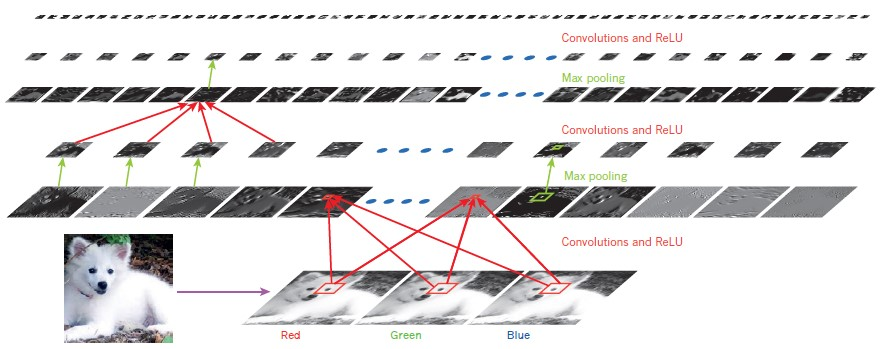
\includegraphics[scale=0.7]{images/chapter_2/CNN.jpg}}
\caption{Convolutional network overview \citep{DBLP:journals/nature/LeCunBH15}}
\label{fig:cnn_overview}
\end{figure}
The architecture of a typical ConvNet (Figure \ref{fig:cnn_overview}) is structured as a series of stages. The first few stages are composed of two types of layers: convolutional layers and pooling layers. Units in a convolutional layer are organized in feature maps, within which each unit is connected to local patches in the feature maps of the previous layer through a set of weights called a filter bank. The result of this local weighted sum is then passed through a non-linearity such as a ReLU. All units in a feature map share the same filter bank. Different feature maps in a layer use different filter banks.

CNN have three great properties which are well suited for processing data that has a known grid-like topology: “sparse interactions”, “parameter sharing” and “equivariant representations” \citep{goodfellow2016deep}. Compared to traditional fully connected layers where every output unit interacts with every input unit, CNNs have sparse interactions. In fact, the size of the convolutional kernel is lower than the size of the input data which means that we need to store fewer parameters, which both reduces the memory requirements of the model and improves its statistical efficiency. Moreover, the same kernel is used throughout grid-like input data, so instead of learning a parameter for each location, only a set of parameters is
learnt. This drastically reduce the number of parameters to learn. With the "equivariant representations" we means the property of CNNs to be equivariant to translations. This implies that if we translate an object in an input image, also its representation produced through the convolutional operation would be translated of the same amount. This property is particularly interesting when we know that some function of a small number of neighboring pixels is useful when applied to multiple input locations. The properties presented above make CNN particularly suitable for working with images. 

Among the many possible applications involving CNNs we remember \textit{Image Classification}, \textit{Object Detection}, \textit{Instance segmentation} and \textit{Semantics segmentation}. Image Classification is a fundamental task that attempts to comprehend an entire image as a whole. The aim is to classify the image by providing it a label. Image Classification often refers to images in which just one item appears and is analysed. Object detection, on the other hand, involves both classification and localisation tasks and is used to analyse more realistic scenarios in which numerous items may exist in an image. Advanced computer vision tasks, instance segmentation, are intended to achieve finer-grained object localisation in input images. The bounding boxes used in object detection find only coarse-grained object boundaries and include many pixels that do not belong to the object. In contrast, instance segmentation improves the object localisation accuracy by identifying each pixel that acts as part of a known object in the image. The semantic segmentation task involves associating each pixel in an image with a class label. In the following subsections we will review 3 different Convolutional based architecture we have used in the course of our research work: \textit{Residual networks} (image classification), \textit{Single Shot MultiBox Detector} (object detection) and \textit{U-Net} (image segmentation).

\subsubsection{Residual networks} \label{Residual Networks}

Most of the state-of-the-art Image classification methods use Residual networks, better known as \textit{ResNet}\citep{he2016deep}. The ResNet architecture solves the vanishing gradient problem for very deep neural network architectures by applying the concept of residual learning. By applying \textit{Shortcut connections} (Figure \ref{fig:shortcut}) it is possible for gradients to propagate further and allow for efficient training of very deep neural networks.

\begin{figure}
\centerline{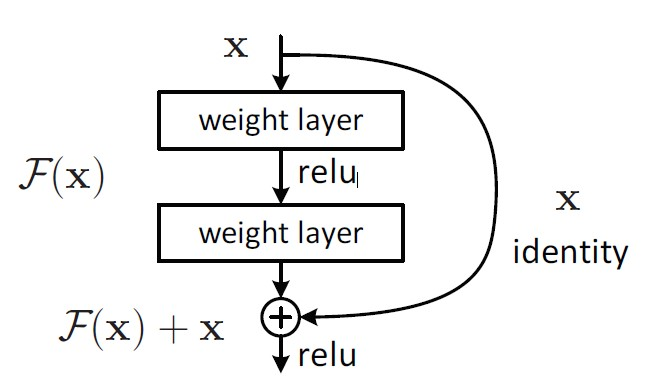
\includegraphics[scale=0.5]{images/chapter_2/residual_learning.jpg}}
\caption{Shortcut \citep{he2016deep}}
\label{fig:shortcut}
\end{figure}

There is empirical evidence that Residual networks are easier to optimise, and can gain accuracy from considerably increased depth. By stacking multiple convolutional layers and by leveraging the concept of residual learning, Residual networks may be very depth with more than 100 convolutional layers. Depending on the number of Convolutional layers, there exists multiples versions of the these models. The most popular architectures are \textit{ResNet18}, \textit{ResNet34}, \textit{ResNet50}, \textit{ResNet101}, \textit{ResNet152}. As shown in figure \ref{fig:resnet_architectures}, the generic ResNet\textit{X} is composed of 5 convolutional building blocks and a last fully connected layer which leverage the extracted features to produce the classification result. Depending on the depth of the architecture each convolutional building is composed of a different number of convolutional layers.

\begin{figure}
\centerline{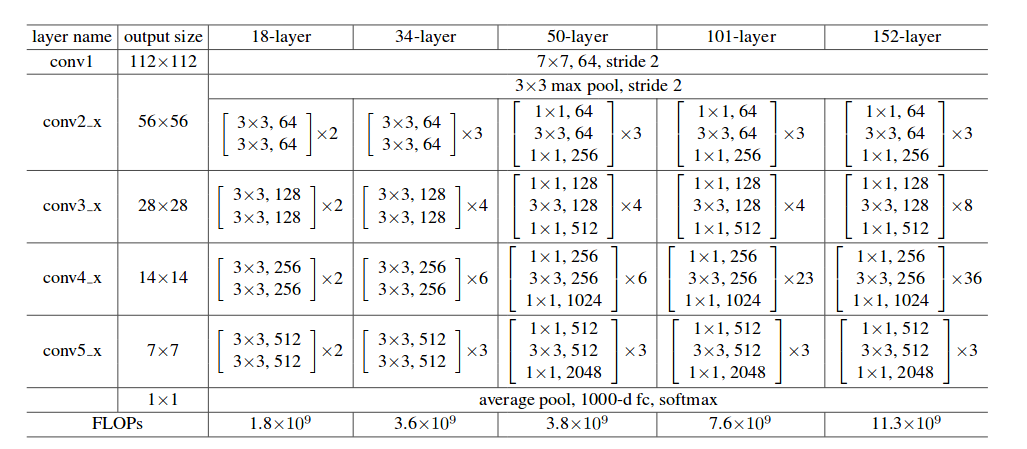
\includegraphics[scale=0.4]{images/chapter_2/resnet.png}}
\caption{ResNet architectures \citep{he2016deep}}
\label{fig:resnet_architectures}
\end{figure}


\subsubsection{Single Shot MultiBox Detector}

Single Shot MultiBox Detector (SSD) (Figure \ref{fig:ssd_architecture}) is a single-stage object detection method that discretizes the output space of bounding boxes into a set of default boxes over different aspect ratios and scales per feature map location \citep{liu2016ssd}. At prediction time, the network generates scores for the presence of each object category in each default box and produces adjustments to the box to better match the object shape. Additionally, the network combines predictions from multiple feature maps with different resolutions to naturally handle objects of various sizes.

\begin{figure}
\centerline{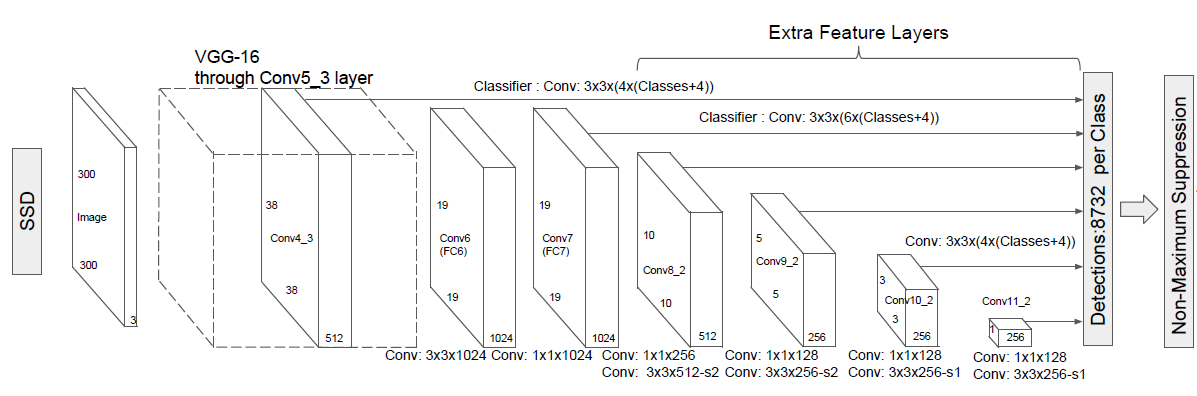
\includegraphics[scale=0.45]{images/chapter_2/ssd_network.png}}
\caption{SSD Architecture \citep{liu2016ssd}}
\label{fig:ssd_architecture}
\end{figure}

This model mainly consists of a base network followed by several multi-scale feature map blocks. The base network is for extracting features from the input image, so it can use a deep CNN. For example, the original single-shot multibox detection paper adopts a \textit{VGG network} \citep{simonyan2014very} truncated before the classification layer. In recent years, other base network architectures have been combined with the multi-scale feature maps blocks. \textit{MobileNet} has been developed to speed up the computation and lends itself well to being combined with the SSD model to perform Object Detection tasks in real-time.  

MobileNet networks \citep{howard2017mobilenets, sandler2018mobilenetv2, howard2019searching} are a family of general purpose computer vision neural networks designed with mobile devices in mind to support classification, detection and more. The popularity these architecture is motivated by the the overall trade-off between the inference speed the model performances.
The main idea behind MobileNet models is based on the concept of \textit{depth-wise separable convolutions}. Depth-wise separable convolutions is a form of factorised convolutions which factorise a standard convolution into a depth-wise convolution and a $1\times1$ convolution called a point-wise convolution. For MobileNets the depth-wise convolution applies a single filter to each input channel. The point-wise convolution then applies a $1\times1$ convolution to combine the outputs the depth-wise convolution. A standard convolution both filters and combines inputs into a new set of outputs in one step. The depth-wise separable convolution splits this into two layers, a separate layer for filtering and a separate layer for combining. This factorisation has the effect of drastically reducing computation and model size \citep{howard2017mobilenets}.


\subsubsection{U-Net}

One popular approach for semantic segmentation models is to follow an encoder/decoder structure where we “downsample” the spatial resolution of the input, developing lower-resolution feature mappings which are learned to be highly efficient at discriminating between classes, and the “upsample” the feature representations into a full-resolution segmentation map. The encoder-decoder approach, as part of the semantic segmentation domain, was proposed for the first time by \citet{long2015fully} in the Fully Convolutional Network (FCN) architecture and it has been subsequently taken up by other research works \citep{ronneberger2015u,zhao2017pyramid,chen2017rethinking,chen2018encoder,badrinarayanan2017segnet}. The encoder, or contracting path, is, most of the time, a Convolutional neural network whose task is to extract features of different spatial resolutions, constituting the so-called “Feature Map”. Compared to the encoder, which reduces the spatial dimension in every layers and increases the channels, the decoder, or expansive path, has the role of restoring the original spatial dimensions by sequentially increasing the spatial dimension while reducing the number of channels. The decoder can be composed of one of multiple decoder block, in the same way the encoder can be more or less deep. Each decoder block computes two different operations: at first it up-sample the feature map using an interpolation method, then it applies a convolutional operation which halves the number of feature channels. Finally, a last convolutional block, sometimes called Segmentation Head, stacked right after the last decoder block produces the segmentation mask. 

One architecture that follows this approach is the \textit{U-net} architecture (Figure \ref{fig:unet_architecture}, proposed by \citep{ronneberger2015u}.
\begin{figure}
\centerline{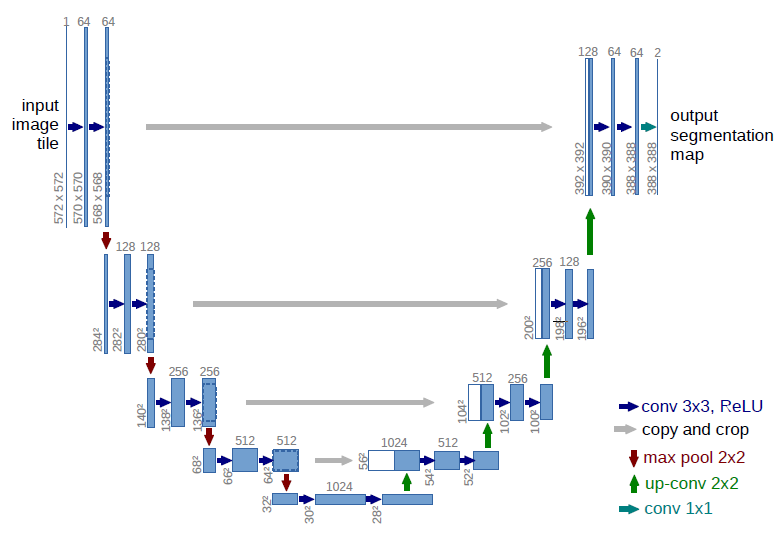
\includegraphics[scale=0.6]{images/chapter_2/unet.png}}
\caption{U-net architecture \citep{ronneberger2015u}}
\label{fig:unet_architecture}
\end{figure}
It consists of a contracting path (left side) and an expansive path (right side). The contracting path follows the typical architecture of a convolutional network. It consists of the repeated application of two 3x3 convolutions (unpadded convolutions), each followed by a rectified linear unit (ReLU) and a 2x2 max pooling operation with stride 2 for downsampling. At each downsampling step we double the number of feature channels. Every step in the expansive path consists of an upsampling of the feature map followed by a 2x2 convolution (“up-convolution”) that halves the number of feature channels, a concatenation with the correspondingly cropped feature map from the contracting path, and two 3x3 convolutions, each followed by a ReLU. The cropping is necessary due to the loss of border pixels in every convolution. At the final layer a 1x1 convolution is used to map each 64-component feature vector to the desired number of classes. In total the network has 23 convolutional layers.

Even if this architecture has been surpassed by more complex methods, constitutes a good trade-off between results accuracy and model complexity, allowing its use in contexts where the size of the training set is not particularly large.


\subsection{Recurrent neural networks} \label{Recurrent Neural Network}

Recurrent Neural Networks (RNN) \citep{rumelhart1986learning} are a family of neural networks that possess internal state or short-term memory due to recurrent feed-back connections, that make them suitable for dealing with sequential problems. The main advantage of RNN compared to others neural network architectures is their ability to process sequences of any length by keeping into account the historical information. More effective sequence models used in practical applications are called \textit{gated RNNs}. These include the \textit{LSTM} (Long-Short-Term-Memory) \citep{hochreiter1997long} and \textit{GRU} (gated recurrent unit) \citep{cho2014properties}. Without going into much details, gated RNNs are based on the idea of creating paths through time that have derivatives that neither vanish nor explode \citep{goodfellow2016deep}. The LSTM has been found extremely successful in many applications, such as speech recognition \citep{graves2013hybrid}\citep{graves2014towards}, machine translation \citep{sutskever2014sequence} and image captioning \citep{kiros2014unifying}\citep{vinyals2015show}\citep{xu2015show}. Thanks to its ability to deal with sequential data, RNN based networks have also been applied reasonably to time series regression/classification tasks \citep{smirnov2018time}.  

\section{Model Hyper-parameters fine-tuning}

The algorithms presented in the previous section have several dozen hyper-parameters. Their adjustment is often crucial to obtain a satisfactory performance. This is called hyper-parameter optimisation: the aim is to optimise the performance of the model for the task at hand. It is also necessary to select the right data preparation methods. This is particularly true for deep learning architectures when the number of hyper-parameter is important. Table \ref{tab:hyper-parameters} summarises the most critical Hyper-parameters to fine tune while training a deep neural network.

\begin{table}[]
\label{tab:hyper-parameters}
\begin{tabular}{|l|p{4cm}|p{4cm}|}
\hline
\textbf{Hyper-parameter}           &  \textbf{Common values applied in scientific literature}  & \textbf{Description}                                    \\ \hline
Number of layers          & {[}2;200{]}                                     & Number of layers in the architecture.           \\ \hline
Layer type                & Fully-connected, Convolutional, Recurrrent, ... & Neural network layer family                                               \\ \hline
Number of Neuron per layer & {[}1;4000{]}                                    & Number of Neuron composing a layer.                                               \\ \hline
Activation function       & ReLu, Softmax, Sigmoid, Tanh, ...               & Function which define the output of the neuron in a range of values.                                                \\ \hline
Cost function             & MSE, MAE, \textit{Hinge} Loss, Categorical cross-entropy, \dots                                                & Function which measure the error between the prediction and the ground truth value.                                               \\ \hline
Weight initialisation     & Random initialisation, \textit{Xavier} initialisation \cite{glorot2010understanding}, \textit{He} initialisation \citep{he2015delving}, \dots                                                & The method applied to initialize model weights. \\ \hline
Learning rate             & {[}$10^{-10}$;$10^{-1}${]}                                                  &  Amount that the weights are updated during training.                                               \\ \hline
Mini-batch                & {[}2;256{]}                                     & Equally sized subset of data over which the gradient is calculated and weights updated.                                               \\ \hline
\end{tabular}
\caption{Most known Hyper-parameters for training a deep neural network}
\end{table}

Methods for automatic optimisation of these hyper-parameters have been proposed. There exists today many Open Source optimisation frameworks that allows to perform this optimisation tasks in an easy manner. Among them we can mention \textit{Optuna} \citep{optuna_2019} that we have used throughout our research work. \textit{Optuna} provides an easy interface to automate the hyper-parameter search. It supports the following sampling algorithms: \textit{Grid and Random Search} (\ref{Grid and Random search}), \textit{Tree-structured Parzen Estimator} (\ref{TPE approach}).


\subsection{Grid and Random search} \label{Grid and Random search}

In order to perform the optimisation, the performance of the method over the range of values of each of the hyper-parameters needs to be evaluated. It is possible to evaluate the whole value range exhaustively, by a regular test grid, which is computationally expensive. A less costly approach in term of calculation time is the random drawing over the range of values, proposed by \citep{bergstra2012random}. 
\begin{figure}
\centerline{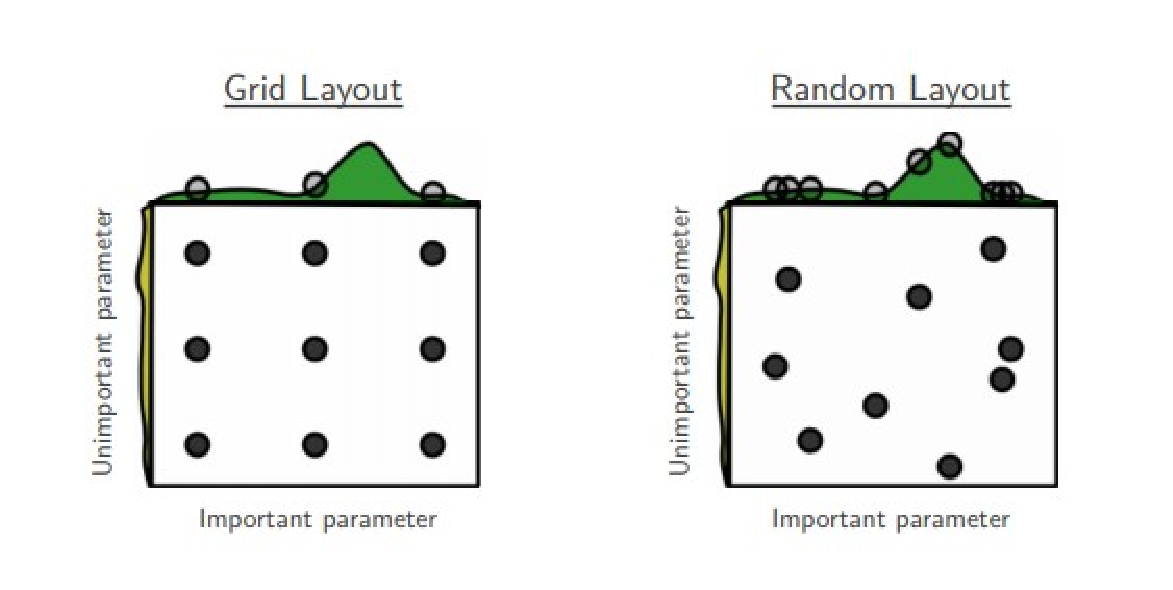
\includegraphics[scale=0.7]{images/chapter_2/random_search.eps}}
\caption{Grid and Random Search \citep{bergstra2012random}}
\label{fig:Grid and Random Search}
\end{figure}
In Figure \ref{fig:Grid and Random Search} the Grid search and Random search of nine trials are compared for optimising a generic function $f(x, y) = g(x) + h(x)$ where Above each square $g(x)$ is shown in green, and left of each square $h(y)$ is shown in yellow. With grid search, nine trials only test $g(x)$ in three distinct places. With random search, all nine trials explore distinct values of $g$. This failure of grid search is the rule rather than the exception in high dimensional hyper-parameter optimisation.

\subsection{Iterative Methods}

In 2011, \citep{bergstra2011algorithms} carried out a state of the art of hyper-parameter optimisation methods for deep neural network models. This work shows the interest of iterative optimisation, based on the criterion of the Expected Improvement of the model performance, proposed by \citep{jones2001taxonomy}. The study introduces two optimisation methods. One method seeks to model the optimisation problem by \textit{Gaussian stochastic processes} (GP) and the second TPE (\textit{Tree-structured Parzen Estimator}) method proposes a kernel-based modeling. These methods are based on the construction of meta-models. The study highlighted the superiority of these two methods over the optimisation by random sampling. In the context of this research work we applied solely the TPE algorithm.

\paragraph{TPE approach} \label{TPE approach}

The Tree-structured Parzen Estimator (TPE) is a sequential model-based optimisation (\textit{SMBO}) approach. SMBO methods sequentially construct models to approximate the performance of hyper-parameters based on historical measurements, and then subsequently choose new hyper-parameters to test based on this model. The TPE approach models $P(x|y)$ and $P(y)$ where x represents hyper-parameters and y the associated quality score. $P(x|y)$ is modelled by transforming the generative process of hyper-parameters, replacing the distributions of the configuration prior with non-parametric densities.

In this subsection we have shown how the hyper-parameters can be optimised. Whether it is carried out through a Random sampling approach or through the use of iterative methods, hyper-parameter optimisation it is an expensive task in term of computation time. The cost of optimising these models is very high, due to the infinity of possible architectures and the many hyper-parameters, especially for neural networks. In the following subsection, we will present an approach that allows for reducing the overall computational time and which facilitates the convergence of the model, especially if the number of samples composing the training set is not particularly high.


\subsection{Transfer Learning} \label{Transfer Learning}

Transfer learning is biologically motivated by the way that humans apply learned knowledge to solve new problems, and consists in exploiting knowledge learned in one problem and searching a good protocol of transferring to a new problem.
In practice, in transfer learning problems, a parametric model is trained in the source problem and transferred to the target problem in a special way, like transferring parameters, or considering the relations between problems. This approach become particularly interesting when we deal with a dataset where the number of samples is small. There is no a well-defined rule to distinguish between a small and a large dataset. Moreover, the amount of data required to solve a machine Learning problem depends on the task that we try to accomplish. In the context of this research project we consider as small, every dataset that have less than 1000 samples. 

Convolutional networks are broadly applicable in the fields mentioned before. The success of transfer learning with convolutional networks relies on the generality of the learned representations that have been constructed from a large database like ImageNet \citep{deng2009imagenet}. \citep{yosinski2014transferable} quantified the transferability of these pieces of information in different layers, e.g. the first layers learn general features, the middle layers learn high-level semantic features and the last layers learn the features that are very specific to a particular task. \citep{zeiler2014visualizing} also visualised the features in the intermediate layers, demonstrating, with images, that convolutional networks learn features from general level to task-specific level. Overall, the learned representations can be conveyed to related but different domains and the parameters in the network are reusable for different tasks. The intuition behind transfer learning for image-related tasks is that if a model is trained on a large and general enough dataset, this model will effectively serve as a generic model of the visual world. You can then take advantage of these learned feature maps without having to start from scratch by training a large model on a large dataset.

In practice, we distinguish two successive stages in the training of a neural network by transfer learning: the training of the new last layers, and then the specialisation of the whole network. The first stage is to guarantee the convergence of the classifier on the new task. We seek to obtain a satisfactory inference score. This is why in a first step, only the weights of the neurons of the new last layers are adjusted by back-propagation of the error gradient. Once the convergence of the last layers has been obtained, it is possible to fine-tune the whole network by performing an adjustment of all the weights of the layers in order to improve the classification score.


\section{Conclusion TO BE FINISHED}

% This chapter allowed us to present our first contributions. A review of the literature on process control and quality improvement in the context of Extrusion Blow-Molding.

\subsection{Scientific Contribution TO BE FINISHED}

\subsection{Industrial Contribution TO BE FINISHED}




% Chapter 3
\setcounter{mtc}{6}
\chapter{From corrective to predictive process control} \label{From Corrective to Predictive Process Control}
\minitoc

\section{Introduction}

In this chapter, we propose an application of the previously proposed method to the industrial context studied in this research project. Since tank weight out of tolerances limits is the first cause of part non-conformities, we have decided to focus initially on the comprehension of the tank weight variability. We are interested in understanding what process parameters contribute most to the variability of tank weight. Firstly, it is necessary to have a representative data set of the phenomenon to be modeled. Subsequently, we will try to leverage the historical set of data to try to model the relationship between the process conditions and the quality of the parts. Results, as well as the difficulties of applying such an approach in the studied industrial context will be discussed in details. Finally, we will show how the results obtained through this research work has made it possible to identify some areas of improvement in the manufacturing process. 


\section{Motivation}

Poor quality or ``scrap'' parts are very expensive for a company like Plastic Omnium Clean Energy Systems. The “Cost of Non-Quality” (CNQ) is one of the key indicators most used by the company. However, when a part is bad, it is first necessary to understand the origin of the problem, which can require a lot of time and energy. Historically, Plastic Omnium industrial process monitoring has been driven using a knowledge-based corrective approach (Figure \ref{fig:Corrective process control}). The quality measurements of each product is used to adjust the process and to maintain the process capability. Moreover, some of the process parameters, which are considered as critic for process safety, are kept under control through the use of uni-variate control charts.  When a parameter falls outside the control limits, some warning messages are generated to alert the operators who have the task of regulating the machine so that the parameter can return in the safe zone. 

\begin{figure}
\centerline{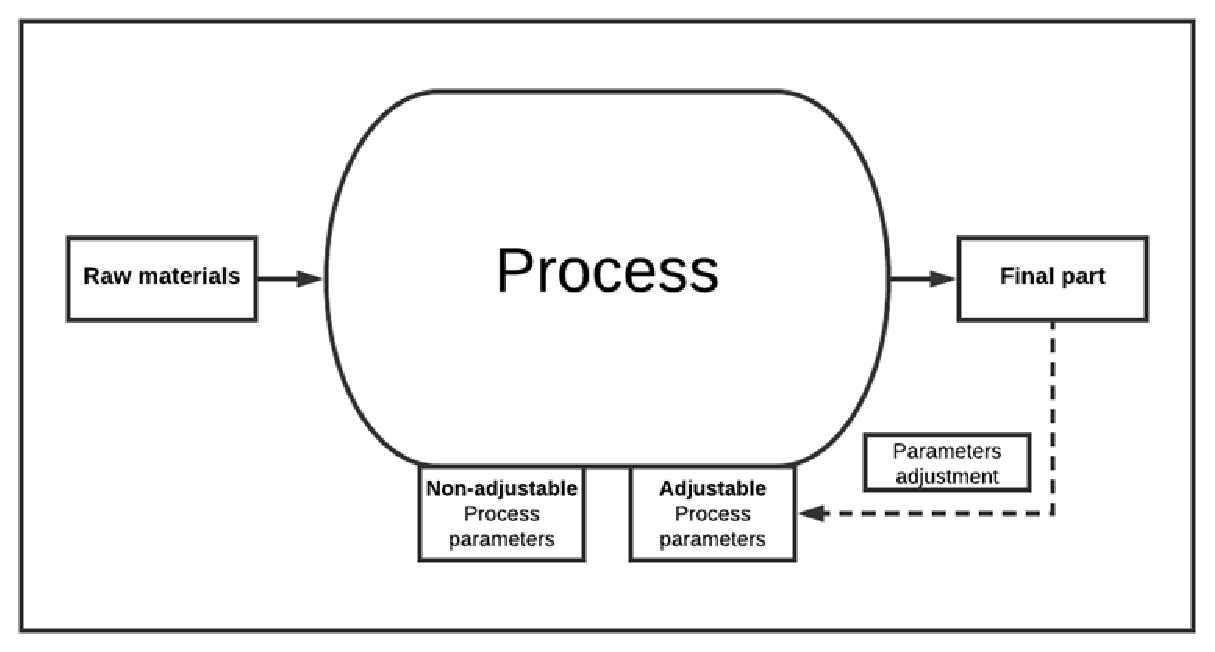
\includegraphics[scale=0.7]{images/chapter_3/corrective_approach.eps}}
\caption{Corrective process control}
\label{fig:Corrective process control}
\end{figure}

Evidence has shown how the overall process stability ensures, in most cases, the product quality stability. However, it still remains unclear how the system parameters affect the product quality variability. Moreover, quality prediction can offer the possibility to define better system parameters at an early production stage. In other words, the product quality anticipation may be used to adjust the process in real time and not retrospectively (Figure \ref{fig:Predictive process control}). Such an approach would allow the product failure anticipation and the just-in-time process correction with an overall reduction of the non-conforming parts.

\begin{figure}
\centerline{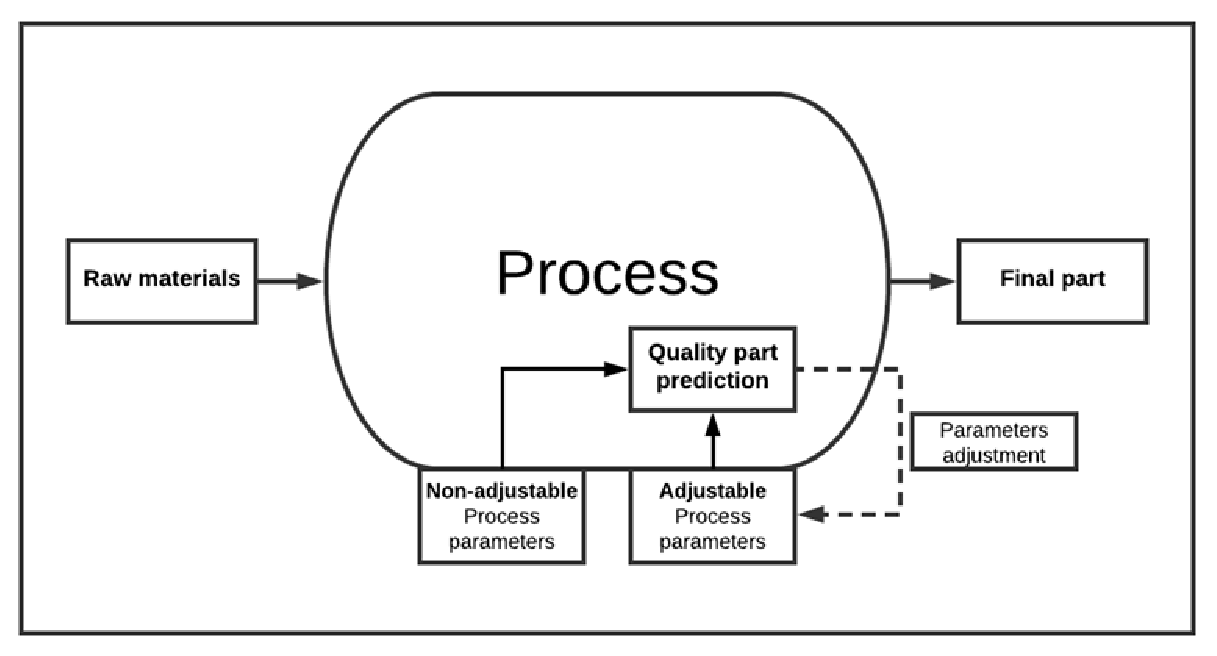
\includegraphics[scale=0.7]{images/chapter_3/predictive_approach.eps}}
\caption{Predictive process control}
\label{fig:Predictive process control}
\end{figure}

In order to understand the relationship between process parameters and the quality of final part, we use a supervised learning approach. We view our complex industrial process as a black box with multiple inputs and one output. Given $p$ process parameters $(X_1,X_2,\ldots,X_p)$ and one product quality variable $Q$, we look for the function that better approximates the relationship between the inputs and the output. Mathematically speaking, we look for the function $\hat{f}$ that approximates the relationship between the process variables and the quality result so that the following expression is verified:

\begin{equation}
    Q = \hat{f}(X_1,X_2,\ldots,X_p) + \epsilon
    \enspace,
\end{equation}
where $\epsilon$ is

By an automatic analysis of a set of examples (training set) of measured input-output behaviour of the process learning algorithms can find out important correlations between process variables and construct classifiers for detecting dangerous or unwanted process states.

In the context of our research framework, a work has been carried out to determinate what are the main causes of scraps involving the Extrusion-Blow Molding process. An analysis conducted on three years of data collected by the Manufacturing Execution System (MES) software of the company in a French plant has highlighted that the first cause of scraps in blow-molding machines is due to tanks whose weight does not meet the customer's specifications. This kind of non-compliance accounts for about one half of the total amount of scraps (Figure \ref{fig:Most common scrap causes (2017-2018-2019)}) followed by inclusion and others contamination problems. 

\begin{figure}
\centerline{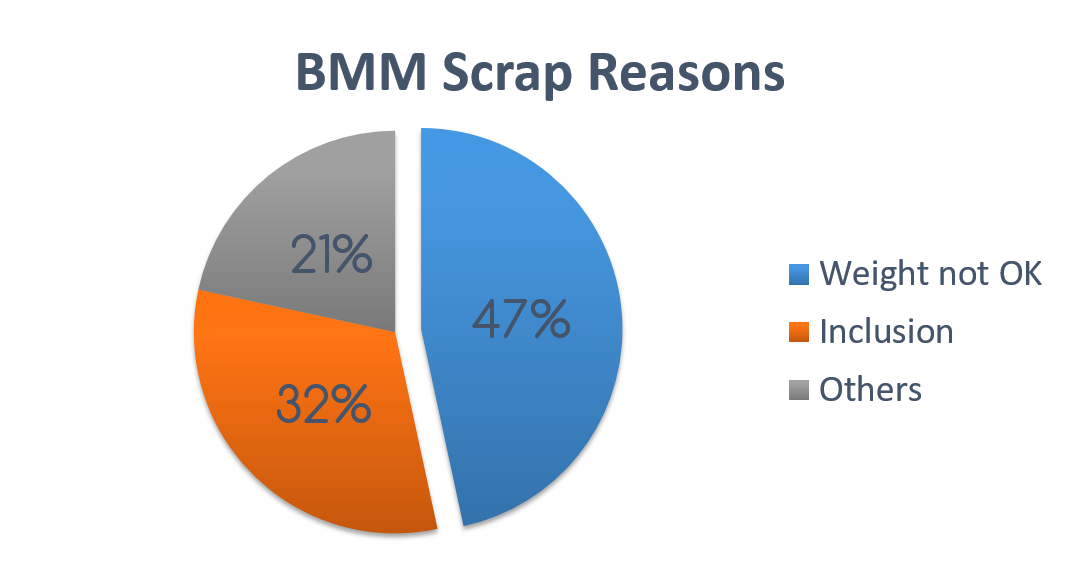
\includegraphics[scale=0.9]{images/chapter_3/Scraps_codes.eps}}
\caption{Most common scrap causes (2017--2019)}
\label{fig:Most common scrap causes (2017-2018-2019)}
\end{figure}

As we have presented in section \ref{The key quality characteristics of a blow-molded fuel tank}, the tank weight is historically considered as an important product characteristic as it provides an overall indication about the amount of material which compose the fuel tank. By ensuring a lower tolerance limit of the weight it is possible, according to experts, to ensure that there is enough material to ensure compliance of thicknesses. In the same way, there exist an upper tolerance limit which exists to ensure that the part it is not to heavy. By measuring in real-time, for each part produced, the weigh of the tank, people in plants feel reassured about the correct material distribution along its surface.  
As a consequence of this analysis, we decided to focus our efforts on trying to understand where these scrap come from and what we can do to try to reduce them. Moreover, since the weight is measured in real-time, it is possible to easily assemble a dataset composed of multiple samples. By following the approach described in section \ref{Proposed Method} of this chapters, we aim to search for any hidden pattern or correlation within process data and quality data that could explain why some parts are not compliant in term of weight.


% \section{Proposed method} \label{Proposed Method}

% In this section, we will try to describe a general framework that can be applied to improve process control. We use supervised machine learning to discover some patterns between the process parameters and the quality of the part that has been manufactured by the same process. We proceed in four main stages:
% \begin{enumerate}
%     \item \textit{Data collection} consists in retrieving all the data needed to model the manufacturing production process. It involves two main stages:  data acquisition and  data labelling (Section \ref{Data Collection}). 
%     \item \textit{Data processing} covers the range of operations required to make the input data suitable for the machine learning algorithm (Section \ref{Data Processing}). 
%     \item \textit{Exploratory data analysis} is an ensemble of graphical and quantitative techniques that can be used to explore data and retrieve important information (Section \ref{Exploratory Data Analysis}).
%     \item \textit{Data modelling} corresponds to the statistical modelling of the relationship between the process data and the quality data by a machine learning algorithm (Section \ref{Machine Learning modeling})
% \end{enumerate}
% %
% \begin{figure}
% \centerline{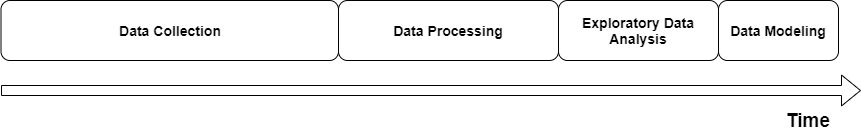
\includegraphics[scale=0.45]{images/chapter_3/stages.png}}
% \caption{The 4 stages towards predictive process control}
% \label{fig:4_stages}
% \end{figure}
% %
% In the remaining part of the current section we will review in details how to carry out these four steps to achieve a \textit{predictive process control}. 

% \subsection{Data collection} \label{Data Collection}

% Collecting data allows to capture a record of past events so that we can use data analysis to find recurring patterns. In the context of this research work, data collection is the task of retrieving the data that could be meaningful to explain the variability of a quality characteristic given some process parameters. Among the many challenges in Industry 4.0, data collection is becoming one of the critical bottlenecks. It is known that the majority of the time for building end-to-end data-driven models is spent on preparing the data, which includes collecting, cleaning, analyzing, visualizing, and feature engineering. Moreover, as machine learning is used in new applications, it is usually the case that there is not enough training data. Traditional applications of machine learning like machine translation or image object detection rely on huge quantities of training data that have been accumulated for decades. On the other hand, more recent applications, especially in the manufacturing industry, have little or no training data. To train a machine learning model, it is necessary to have samples that are representative of the entire operating range of the process. If the individuals do not cover the whole process functioning, the model will be biased.

% Two kind of data are required: the input data, corresponding to the process data and the output data which is actually the measure of the quality of the parts. Data collection involves mainly two different steps: \textit{process data acquisition} and \textit{Quality data acquisition}. 

% \subsubsection{Process data acquisition} \label{Process Data Acquisition}

% We use here the term \textit{process data} for any type of data belonging to the manufacturing process. For instance, some process data of the extrusion blow-molding process are the extruder throughputs, the extruder temperature, or the  blowing air pressure. This process data is a picture of the state of the process at a given time.

% Process data acquisition is a challenging task in Industry 4.0 due to different technologies, machines, sensors, IoT devices and communication networks. Sensors, actuators, and PLCs are the main data generators in the automotive industry \citep{khan2017big}. In the last decade a new type of intelligent sensor, also called \textit{smart sensors}, is more and more used in the manufacturing industry. Most of the data available in the Manufacturing plants comes from PLCs, sensors and smart sensors. The three devices are further explained as below.

% \begin{itemize}
%     \item \textit{Sensors} convert a physical state or activity into an electrical signal that is sent to the PLC for further processing. In manufacturing, sensors create a huge amount of data. Most machines and robots include sensors that collect data from their surroundings, such as the temperatures of a machine or its environment.
%     \item \textit{Smart sensors} are devices that take information from a physical environment and use embedded microprocessors and wireless communication to monitor, examine and provide information about the proper functioning of the observed system. With the developments of the IoT and machine learning, various types of smart sensors are nowadays available. They are massively applied in the manufacturing industry and they provide a lot of information that can be used in the task of better controlling the process and to better understand the quality part variability.
%     \item \textit{Actuators} controlled by the PLC, produce a physical action. A basic example of an actuator connected to a PLC is the automatic starting of a motor. There are several robots for automated procedures in the industry. These robots are actuators that produce a large amount of data.
%     \item \textit{PLC} is a programmable unit that takes input from sensors, and controls actuators (Figure \ref{fig:plc}). A factory has has a large number of PLCs based on the processes. PLCs are manufactured by different suppliers and they generate heterogeneous data which is a big challenge for industrial big data.
% \end{itemize}

% \begin{figure}
% \centerline{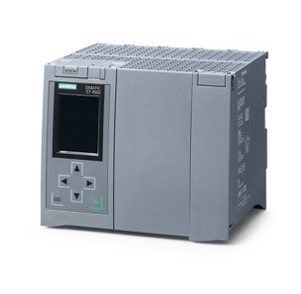
\includegraphics[scale=1]{images/chapter_3/PLC.jpg}}
% \caption{PLC \textit{Siemens} S7-1500}
% \label{fig:plc}
% \end{figure}


% The presented devices produce a lot of data but they do not manage the data storage. In fact, PLCs have a limited amount of storage space and they cannot be used to store the data permanently. The local machine data storage is most of the time handled by the SCADA (Supervisory Control And Data Acquisition) software. The term SCADA is used to identify any kind of software, installed on a personal computer or server, which allows the implementation, operation and management of supervisory, control and remote control systems without necessarily having to write code using programming languages. SCADA software have multiples functionalities which range from automation, to alarm handling, logging, archiving and simple statistical analysis \citep{daneels1999scada}. SCADA is a powerful system for acquisition of industrial automation data but, it is not able to handle the storage of a large volume of data. For this reason the collected data through the SCADA system should be stored elsewhere, in a place where data are easily accessible. Cloud platform, whether they are internal the manufacturing company or outside, are generally the solution for storing a large amount of data. Cloud platforms, or \textit{data Lake}, has been designed to be highly scalable and it provides a way to easily access the data through Big data technology that facilitate and accelerate the data analysis stages.  

% In order to be able to properly manage the data acquisition, taking into account the heterogeneity of the data coming from the different data sources, we propose to introduce a \textit{Gateway} system which constitutes an intermediary bridge between the shop floor PLCs, ans sensors, and the Cloud platform where the data are stored. Moreover, it can communicate with the \textit{MES} system. The Manufacturing Execution System (MES) is a production management system serving as the information center in the enterprise to improve manufacturing transparency. It is the middle layer connecting the manufacturing process on the shop floor and the business process on the Enterprise Resource Planning (ERP) \citep{chen2020implementation}. By communicating with the MES system, it is possible to associate to a produced part the set of events that have enabled its production.

% The architecture of the overall data acquisition system is visible in Figure \ref{fig:data_acquisition_architecture}.

% \begin{landscape}
% \begin{figure}
% \centering
% 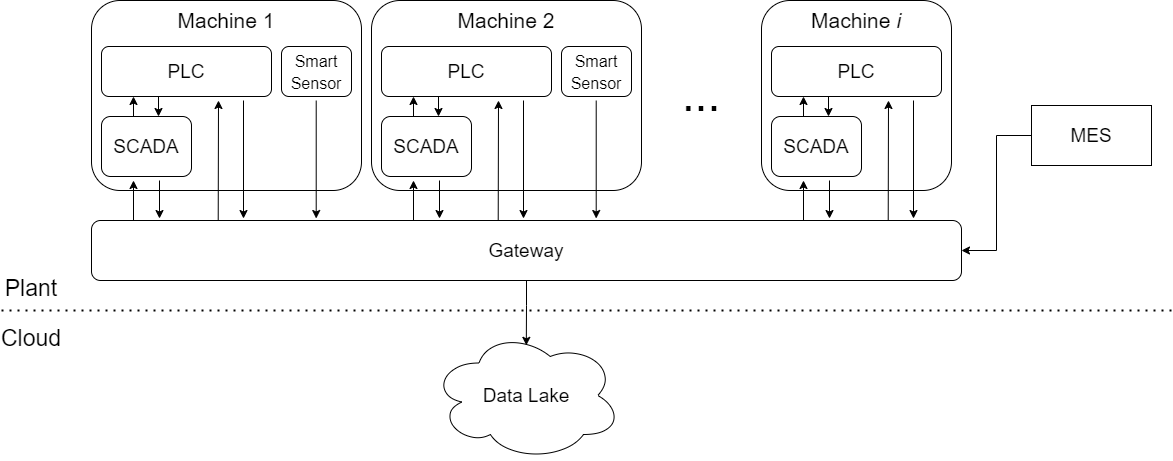
\includegraphics[scale=0.5]{images/chapter_3/Data_acquisition_architecture.png}
% \caption{Data acquisition architecture}
% \label{fig:data_acquisition_architecture}
% \end{figure}
% \end{landscape}

% The gateway is a physical or virtualized server which acts like an intermediary between the data acquisition systems available in the shop floor and the Cloud platform where the data are stored for data analysis. The gateway connected to the shop floor network and it is able to interact directly with the PLC of the machines as well as smart sensors.  

% The gateway has two main roles:

% \begin{itemize}
%     \item It allows to centralize the data collection at the plant level. It is in charge to retrieve the data from all the data sources, whether they are PLCs, smart sensors, SCADA software or the MES system. This process facilitates the subsequent sending of data to the Cloud platform. 
%     \item This gateway is well suited for eventually deploying in production at the plant side the machine learning models that have been trained. 
% \end{itemize}

% The gateway should be equipped with different tools and software to allows the communication with the machines through the different communication protocols mainly used in Industry 4.0. There exist a multitude of communication protocols. Among all these we can mention \textit{OPC UA} and \textit{MQTT}. OPC UA (Open Platform Communications Unified Architecture) is a service-oriented machine-to-machine communication protocol mainly used in industrial automation. Its main goals are to provide a cross-platform communication protocol while using an information model to describe the transferred data \citep{profanter2019opc}. MQTT (Message Queuing Telemetry Transport) is an open message protocol which mainly focuses on a small code footprint and low network bandwidth usage, while handling high latency or bad network connections \citep{profanter2019opc}. Further information regarding the communication protocols used in Industry 4.0 are available in \citep{profanter2019opc}\citep{8262021}\citep{zezulka2018communication}.


% \paragraph{Process data types}

% When dealing with process data, we distinguish two different types of data: \textit{Cyclical data} and \textit{Time series data}.

% \begin{itemize}
%     \item \textit{Cyclical data}: Cyclical data are scalar values which provide information about a certain recurring event. Examples of Cyclical data are the machine cycle time, or the time needed from the machine to perform an operation. 
%     \item \textit{Time series data}: Whenever a production process, or a part of it, requires time to be completed, it is possible to recover multiple sequential values of the same process parameters. This sequence of sequential data take the name of time series. The number of sequential values composing the time series depends on the sampling rate and may change accordingly to the nature of the measurement. For instance, the temperature of a machine components may be measured all along the production cycle and it is a classical example of time series data.
% \end{itemize}

% \begin{figure}
% \centering
% 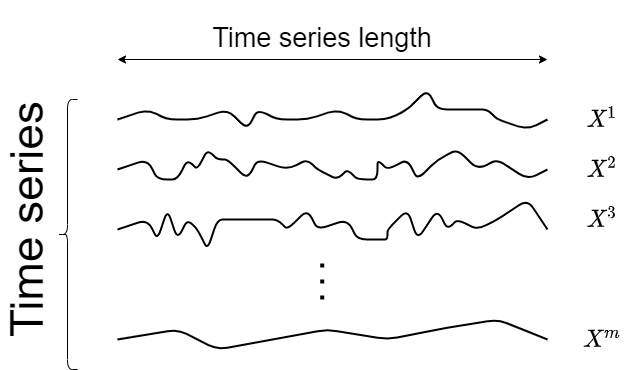
\includegraphics[scale=0.5]{images/chapter_3/time_series_data.png}
% \caption{Time series data}
% \label{fig:time_series_data}
% \end{figure}


% \subsection{Quality data acquisition}

% Quality data acquisition is the task of collecting product quality data associated with all or some of the parts produced. The quality label can be continuous or discrete depending on the applied measurement method. For instance, we can measure a thickness of a manufactured part and provides the results in the form of continuous values in meters. On the other hand, we can measure a thickness value and associate it to  a class according to its compliance, or non-compliance with the specifications. Accordingly to the type of the label, either discrete or continuous, the data modelling may change. If the label is discrete the supervised learning modelling takes the form of a Classification problem (\ref{Classification}), otherwise it will be treated as a Regression problem (\ref{Regression}).   

% The quality data acquisition can be done offline or online. The following two paragraphs will provide an overview of these two methods. 


% \paragraph{Offline acquisition}

% Offline acquisition, is the most common approach for labelling manufacturing data. In fact, for all non-visual product characteristics, it is extremely complicated to asses the quality of a part in less then a minute. Most of the quality controls realized on the part require specific equipment and the task of controlling the part can take several minute. Moreover, effective controlling might result in the destruction of the product or render it unfit for sale in some way. In such a case, the only possibility is to measure the quality of the part offline. Measuring offline has the advantage of allowing careful control of the manufactured parts, reducing the possibility of measurement error. However, as there are only a few parts to measure, it may takes a long time to build a dataset which is representative of all categories of part non-compliance.

% Since, we are not able to measure the quality of all parts produced, it becomes crucial to structure the data collection to make them easily usable for future data analysis. Data have to be stored in a database and the quality measurement must be related to a part number, or traceability number, in order to subsequently associate it with the process data, which in turn must be tagged with the part number. 


% \paragraph{Online acquisition}

% Performing the online data acquisition, on the production line, eliminates two critical error risks:
% \begin{enumerate}
%     \item The loss of the link between the production measurements and the off-line annotation.
%     \item The transformation of the parts between their production and their annotation.
% \end{enumerate}

% On the other hand, the time available for the annotation is very limited. Most of the time the machine operators have time constraints to meet the production cadence. As a consequence this data annotation must be done in a limited amount of time. Depending on the operator task the available time for performing the control may change. We estimate that the operator can consecrate a maximum of one third of the production cycle time to this task, which means that for a process with a cadence of 60 seconds the operator has at maximum 20 seconds to perform this task. In addition to the annotation time, the human expert has to assist in the handling of the parts and related operations.

% By automating the process data acquisition through the data collection presented above, and by ensuring the proper registration of the quality data obtained by measuring the parts, it is possible to permanently feed a dataset with new data in an automatic manner. Over time we can hope to recover enough data to cover the all distribution of all possible quality non-conformities. 

% \subsection{Data processing} \label{Data Processing}

% As heterogeneous data is collected in manufacturing processes, it becomes necessary to process these data to make them more suitable for data analysis. In general, Data processing is the result of three major tasks: data cleaning, reduction, and scaling.

% \begin{itemize}
%     \item \textit{Data cleaning} aims to enhance the quality of the data by missing value imputations and outlier removals. 
%     \item \textit{Data reduction} is applied to reduce data dimensions and therefore, reducing the computational costs associated. 
%     \item \textit{Data scaling} aims to transform the original data into similar ranges for predictive modelling. 
% \end{itemize}

% In the remaining part of this section we will provide some additional elements regarding these three data processing tasks. 
  
% \paragraph{Data cleaning}

% % Missing literature references

% Data cleaning is the result of two main operations: missing values inputations and outlier removals.

% There are two main approaches to dealing with missing data. The first option is to simply reject data samples with missing values since most data mining algorithms cannot handle missing data. This approach is only useful when the amount of missing values is small. The second technique is to use missing value imputation to replace missing data with inferred values. Mean imputation, forward or backward imputation, and moving average techniques are examples of traditional inputation procedures. In such a case, missing values are inferred based solely on the data properties of that variable, and therefore are referred to as univariate techniques. The mean or median imputation method will replace missing values with the mean or median of that variable. The forward or backward method simply replaces the missing value with the previous or next data measurement. More advanced techniques make use of regression model based methods to obtain more accurate inputation results. 

% As regarding outlier removals, the most commonly used techniques use statistical analysis to identify which data belongs or not to the data distribution. Data outliers can be identified, for instance, if the data fall beyond a certain range constructed using conventional statistics such as standard deviations, means and quartiles. Identifying outliers is a delicate operation as, what at first glance might appear to be an outlier, could turn out to be extremely interesting data. When dealing with manufacturing process data, the outlier can be representative of a process functioning state which is not normal and could therefore explain some product quality non-compliance. Physical knowledge of the production process is therefore indispensable in order to understand whether the outliers are due to a process malfunction or to a data acquisition error.    


% \paragraph{Data Reduction}

% % Missing literature references 

% Assuming that data are ranged in a tabular format where the row represents the samples and columns the features, or process parameters, data reduction may be conducted to reduce either the number of samples or the number of columns.
% There are three main methods of column-wise data variable reduction: The first is to use domain knowledge to directly select variables of interests. The second is to use statistical feature selection methods to select important variables for further analysis. The third is to adopt feature extraction methods to construct useful features for data analysis.
% Human expertise plays a key role in the data acquisition process and, globally, in the task of modelling by statistical learning the relationship between process and product characteristics. For complex process the number of available process parameters are huge, in the order of hundreds and sometimes thousands. The Human experts most of the time has many years of experience working with a particular Manufacturing process and it knowledge of the process may be used to pre-select a number of useful features that can be used to try predicting the target output. 

% As regarding feature selection techniques, we distinguish mainly three approaches: the filter, wrapper and embedded methods. The filter method is a simple feature selection approach in which variables are ranked and selected based on specific univariate metrics. Pearson's correlation coefficient is a common filter technique for determining the direction and strength of a linear relationship between two variables. A wrapper method may be used to assess the usefulness of data variables given a certain learning algorithm. Heuristic search methods, such as stepwise forward and backward selection methods, are commonly used. When compared to the filter approach, the wrapper method can take into consideration data variable correlations and interactions with learning algorithms. However, because it is generally performed via an exhaustive search, the computing costs associated with it might be significantly higher. The embedded technique has been developed to optimize the feature selection result via the model training process in order to decrease computation costs. Two popular embedded methods are the L1 regularization (based on the least absolute shrinkage and selection operator, LASSO) and L2 regularization (based on ridge regression) (\ref{Parametric models}). By adding the $L1$ or $L2$ regularization terms to the objective function it is possible to use a penalized linear regression to accomplish the feature selection task.

% Unlike feature selection, which picks only relevant features from existing variables, feature extraction seeks to create new features based on linear or nonlinear combinations of existing variables. Most common linear feature extraction techniques include principal component analysis (PCA) and statistical methods. Statistical methods typically calculate summarizing statistics such as the mean, peak, and standard deviation, for data measurements over a particular time span as features. This approach is particularly suited for the time series data. When dealing with time-series data we can compress the entire information in a limited set of new features computed through the use of summarizing statistics. When working with PCA, the features extracted, corresponding to the Principal Components, are linear combinations of the original data variables. The PCA-based method can be very useful when there presents data multi-collinearity problem. In practice, the number of principal components or features extracted is determined based on the proportion of total data variance explained, for instance, the principal components should be capable of explaining at least 80 or 90\% of the total data variance. To minimize the potential information loss, more advanced techniques can be applied. Nonlinear feature extraction such as \textit{AutoEncoders} may be used to extract more complex and useful features.


% \paragraph{Data Scaling}

% Data scaling is often needed to ensure the validity of predictive modelling, especially when the input variables have different scales. The most used scaling techniques are \textit{max-min normalization} and \textit{z-score standardization}. Min-max normalization is defined as follow:
% \begin{equation}
%     x = x - x_{min} / x_{max} - x_{min}
% \end{equation}

% where $x_min$ and $x_max$ refer to the minimum and maximum values of the generic feature x. The z-score standardization is instead defined by the following equation:

% \begin{equation}
%     x = x - \mu / \sigma
% \end{equation}

% where $\mu$ is the mean and $\sigma$ is the standard deviation of the feature $x$.

% Z-score standardization is well suited when data are normally distributed.
% The max-min normalization, instead, is recommended when the data do not conform to a normal distribution and have no outliers. 


% \subsection{Exploratory data analysis} \label{Exploratory Data Analysis}

% Exploratory Data Analysis (EDA) is a set of data analysis techniques that may be applied to:

% \begin{itemize}
%     \item Uncover underlying structures,
%     \item Isolate important variables,
%     \item Detect outliers and other anomalies,
%     \item Suggest suitable models for conventional statistics.
% \end{itemize}

% EDA is usually the intermediate stage between the Data processing and the Data modeling. By exploring the data, it is possible to discover interesting patterns among data and drive the modeling phase depending on what has been observed. Moreover, the EDA allows to fine-tune the Data processing stage. In fact, by exploring the data we can identify useless features that cannot bring any added value and can therefore be discarded.   

% The term “Exploratory Data Analysis” was introduced by John W. Tukey who in \citep{tukey1977exploratory} shows how simple graphical and quantitative techniques can be used to explore data.

% Typical graphical techniques are:

% \begin{itemize}
%     \item Plotting the raw data (e.g., stem-and-leaf diagrams, histograms, scatter plots)
%     \item Plotting simple statistics (e.g., mean plots, box plots, residual plots)
%     \item Positioning (multiple) plots to amplify cognition
% \end{itemize}

% Typical quantitative techniques are:

% \begin{itemize}
%     \item Interval estimation
%     \item Measures of location or of scale
%     \item Shapes of distributions
% \end{itemize}

% A very convenient tool for performing exploratory data analysis is the Principal Component Analysis (section \ref{Principal Component Analysis}). By projecting the input data on the Principal Components, it is possible to visualize most of the input data variance by simply plotting the data to the firsts Principal Components which accounts for the most data variability. In such a way, it is possible to visualize most of the variability of the input data, even if the size of the feature space is not negligible. 

% \subsection{Machine learning modeling} \label{Machine Learning modeling}

% Machine learning modeling involves the use of machine learning algorithm to approximate the transfer function between the input process data and the output quality data. Mathematically speaking, we look for the function $\hat{f}$ so that:

% \begin{equation}
%     Q = \hat{f}(X_1,X_2,\ldots,X_p) + \epsilon
% \end{equation}

% where:

% \begin{itemize}
%     \item $Q$ is the target quality variable we want to infer given the input process parameters.
%     \item $\hat{f}$ is the transfer function approximated through the use of a statistical algorithm.
%     \item $(X_1,X_2,\ldots,X_p)$ is the set of input process parameters.
%     \item $\epsilon$ is an error term which is independent of $(X_1,X_2,\ldots,X_p)$ and which account of the approximation error. 
% \end{itemize}

% Since we are interested both in prediction and inference, we privilege for this task easily interpretable methods such as parametric models and tree-based methods. 

% % rephrase it

% The model training is usually done by applying cross validation and hyper-parameter tuning. Different supervised learning algorithms have to be trained and parameterized to allow a comparison of their performances in order to select the best performing model. 

% As the a-priori selection of adequate algorithms is not achievable in a generalized way \citep{kotthoff2016algorithm}, different learning methods and algorithms have to be compared and evaluated for each individual application \citep{lee2020machine}. The pre-selection must be made on the basis of selected criteria, e.g. complexity, interpretability, and speed. 
% Regarding our use-case of understanding what process parameters affect the most the quality of the manufactured part, the prediction time as well as the potential precision, which is associated with model complexity, are of greater interest. However, algorithm performance is also affected by factors such as the data volume. Since we are interested both in prediction and inference, we privilege for this task easily interpretable methods machine learning algorithms such as Parametric models and Tree-based methods and Support Vector Machines. We claims that deep  learning based methods are not well suited for this task as a consequence of their "black-box" nature.

% For the evaluation and comparison of model performances, different statistical performance metrics can be applied. For binary classifications, the metrics can be calculated based on the entries of a confusion matrix, as shown in Table \ref{tab:confusion_matrix}.

% \begin{table}[]
% \label{tab:confusion_matrix}
% \begin{tabular}{l|l|l|}
% \cline{2-3}
%                                          & Actually Positive              & Actually Negative              \\ \hline
% \multicolumn{1}{|l|}{Predicted Positive} & \textbf{True Positives (TPs)}  & \textbf{False Positives (FPs)} \\ \hline
% \multicolumn{1}{|l|}{Predicted Negative} & \textbf{False Negatives (FNs)} & \textbf{True Negatives (TNs)}  \\ \hline
% \end{tabular}
% \caption{Confusion Matrix}
% \end{table}

% The comparison of the predicted class with the true class allows to distinguish between correctly positive or negative classified examples (true positive, true negative) and incorrectly classified examples (false positive, false negative). This approach is particularly useful when you simply want to discriminate between a non-conforming part (NOK) and a conforming part (OK). If the objective is to predict a continuous numerical value, the supervised machine learning problem should be transformed into a Regression problem. When dealing with Regression, others metrics are used to evaluate the performance of the trained models. Regarding our use-case, we claims that the most suited metrics are $R^2$, $MSE$ and $RMSE$ (ADD REFERENCE TO CHAPTER 2). The advantage of RMSE over MSE and R2 is the ability to provide an error in the same unit of measure of the target variable. For instance, if we are measuring a continuous characteristic such as the thickness of a blow-molded part, the $RMSE$ return the average prediction error in meters, or in any other unit of length. This guarantees greater interpretability of the final result for people not familiar with statistics.

% From a technical point of view, the scoring time of the model should be fast enough to eventually adjust the production process in real-time. The required response time depends, of course, on the manufacturing process. The scoring time is affected not just by the algorithm employed, but also by the hardware and software on which it is implemented. However, we claims that in most situations, the allowed reaction time is sufficiently large that the scoring time limitation does not limit the model selection process.


% In this section our approach to improve the process control has been presented. In the next section, we will provide the results obtained by applying the approach presented above in our industrial context.


\section{Data collection}

The industrial process taken into account has more than 5000 process parameters measured in real-time at each production cycle. Among all this features, some of these are considered as critical to ensure the proper process stability according to experts (compare section \ref{The key parameters of the Extrusion Blow-Molding}). In addition to the critical process parameters there exist other timer and counter variables. A timer variable is a variable which account for the time needed to execute a particular mechanical movement. A machine production cycle requires the movement of several mechanical elements. The time required to execute the movement is recorded. The sum of all the mechanical times corresponds to the machine cycle time. A counter variable, instead, is a variable which increase over time because of a particular event. The number of part produced in a production day is an example of counter variable.  

Process parameters are collected by the internally developed SCADA system and the data are stored in multiple databases in accordance with the sources of the data. For instance, all the extrusion process data are stored database. The same is true for the blow-molding data and for the weight of the tank that are stored in two separates databases. Moreover, each process parameter measured in real-time during the production process has to be associated with the scalar value corresponding to the quality measurement of the manufactured product, at the end of the production cycle. In order to do that, The SCADA software computes some aggregate data to resume the information in a limited set of scalar features. For each data belonging to a production cycle average, maximum and minimum are calculated. Then, the SCADA software attaches the aggregates data belonging to a production cycle to a specific traceability serial number which can be used as key to join together the different sources of data. 

Unfortunately, there is an important parameter that is not collected through the SCADA software, the parison length. As explained in section \ref{Research framework: The Extrusion Blow Molding}, the parison length provides information about the material distribution. The Extrusion Blow-Molding process taken into account in this research work has no system for measuring the parison length. In this next subsection we will present our approach based on Computer Vision to measure the parison length in real-time.

\subsection{Parison length estimation using Computer Vision}

One of the key characteristics which can explain the tank weight variability is the length of the plastic parison when it is closed inside the molds at the beginning of the blow-molding process. In fact, accordingly to the length of the parison the distribution of the thickness may change and this can impact the weight of the final part. The parison length is not available within our process data database because the machine is not equipped with the sensors to measure it. Measuring the length of the parison requires to equip the machine with external sensors. In order to be efficient, flexible and robust, our measuring system should present the following properties:
%
\begin{enumerate}
    \item Have a relatively small software and hardware cost.
    \item Require little to no expert intervention to adapt the model or process the data.
    \item Be rapidly adaptable to a novel or evolving industrial situation. For instance, the system should be easily adaptable to any blow-molding machine in every plant of Plastic Omnium.
    \item Be capable of doing real time analysis.
    \item Be capable to return the result with a low latency.
    \item Be able to run in a hostile environment. 
    \item Be robust to (small) variations in the environment. For instance, the system should be able to function day and night regardless of lighting conditions.
\end{enumerate}
%
In order to take into account the previous industrial constraints, we made the choice to move towards a Computer Vision based approach. Our choice is motivated by the low cost of a camera, compared to others sensors, and by the performances achieved by Deep-Learning based algorithms in detecting object within images. In section \ref{Convolutional Neural Network} we shown how Neural Networks and, in particular, Convolutional Neural Networks reaches stet-of-the-art results in image based classification, object detection and image segmentation tasks. Motivated by the results presented in scientific literature we took the choice of traininig a Convolutional Neural Network able to detect the Parison in real-time and then to provide the length measurement.
The length measurement involves mainly two stages:
\begin{itemize}
    \item The parison detection: the parison should be detected inside the field of view of the camera. A Deep-Learning model have to be trained in order to detect the bounding box containing the parison. 
    \item The length measurement: Once the parison is detected, the length measurement is not trivial as it corresponds to the length of the bounding box or better to the number of pixels between the top and the bottom of the bounding box.
\end{itemize}

In order to achieve real-time length detection we have chosen the \textit{SSD MobileNet-V2} architecture (compare section \ref{Single Shot MultiBox Detector}). The choice of using these architecture is motivated by the the overall trade-off between the inference speed the model performances. 

In order to train such a model, 200 parison images has been collected using a camera of HD resolution ($1280\times720$). By taking images of the parison all along the extrusion we can build a representative dataset of all the possible input data. The images have been subsequently annotated by means of the Open Source \textit{Labelme} software \citep{wada2016labelme} (Figure \ref{fig:input_and_label}). It is therefore possible to retrieve the bounding box containing the object.   

\begin{figure}
\centerline{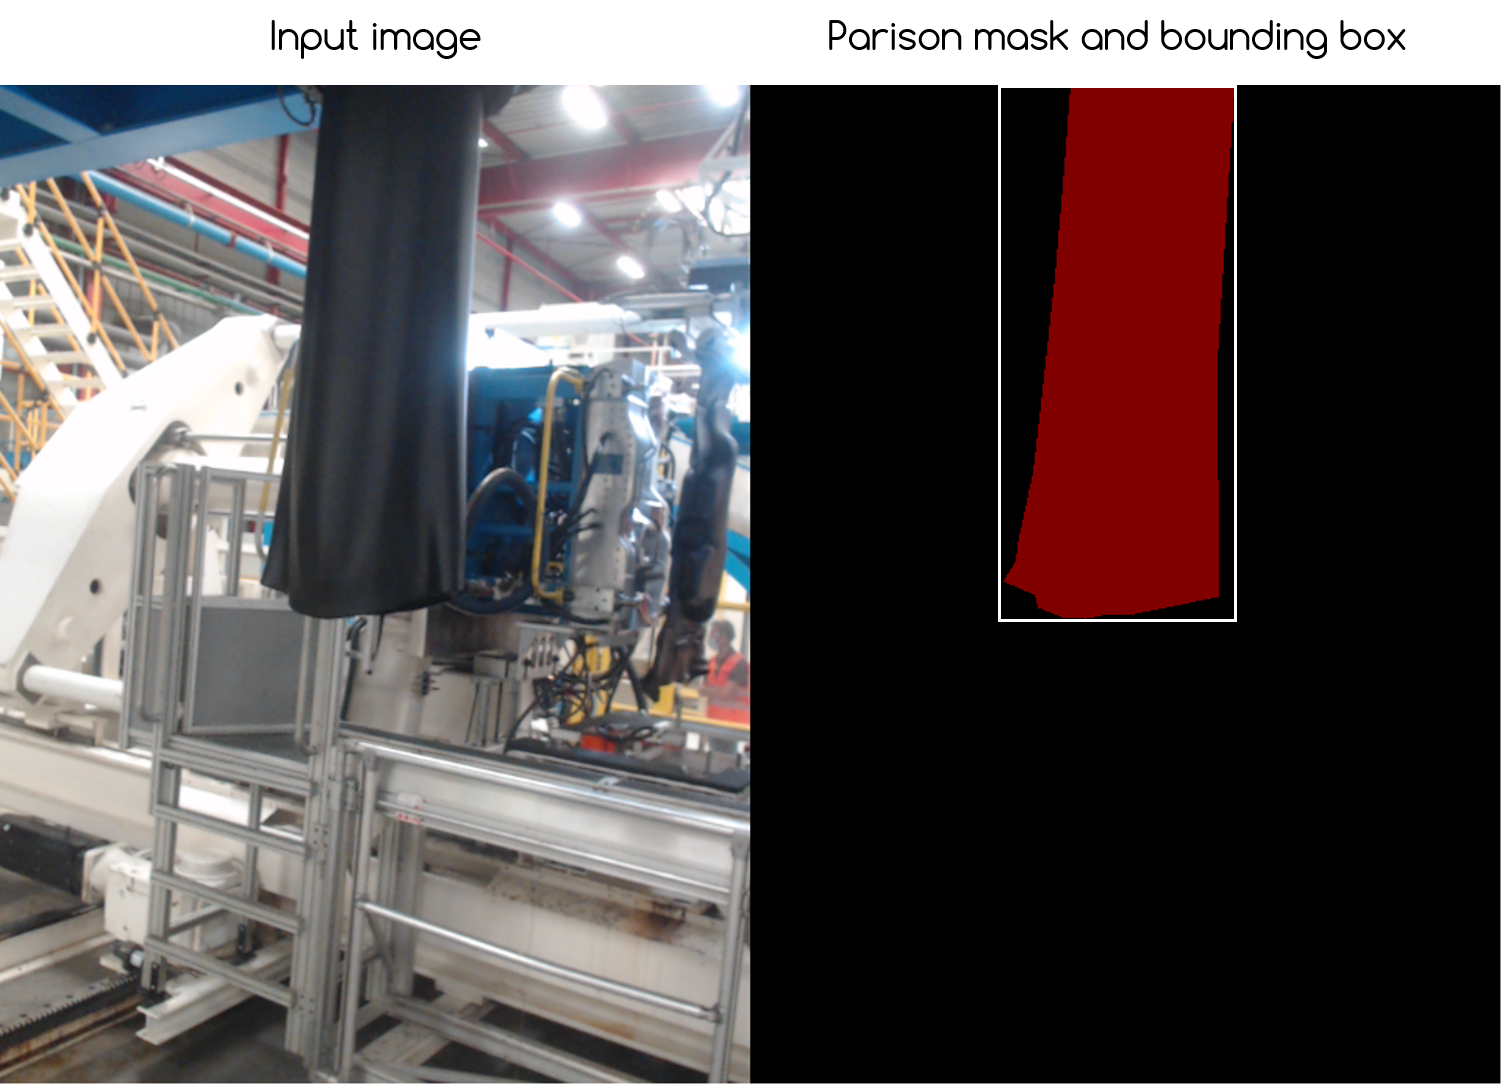
\includegraphics[scale=0.4]{images/chapter_3/input_and_label.png}}
\caption{Input image and parison mask}
\label{fig:input_and_label}
\end{figure}

As regarding the training, the data has been split into three different subsets: the training set (70\%), the validation set (10\%) and the test set (20\%). The training set samples are used to train the model, the validation set is used during the training to evaluate the performance of the model on unseen samples and to eventually stop the training if the model tends to over-fit. The test set constitutes the subset of samples used to evaluate the performance of the trained model on previously unseen data. The architecture has been trained to minimise the loss function using the  \textit{Adam} optimiser~\citep{kingma2014adam} with the default parameter values ($\beta_{1} = 0.9$, $\beta_{2} = 0.98$ and $\epsilon = 10^{-9}$). The loss function used to train such as model is the combination of a \textit{Localisation loss} and a \textit{Confidence loss} The localisation loss is the mismatch between the ground truth box and the predicted boundary box. The confidence loss is the loss of making a class prediction. For every positive match prediction, we penalise the loss according to the confidence score of the corresponding class.
% SHOULD I ADD MORE INFORMATION ABOUT THE LOSS ?

Due to the limited number of samples composing our dataset, 200 images are considered a really small dataset for a deep-learning based computer vision task, we decided to take advantage of a pre-trained Neural Network. By leveraging transfer learning (compare section \ref{Transfer Learning}) it is possible to converge faster to an optimum solution even if the size of the input data is limited. Instead of training the model from scratch, our architecture is initialised with the pre-trained coefficients on the \textit{COCO} dataset \citep{lin2014microsoft}. The last linear layer of the model has been replaced with a new one in order to be consistent with the number of the expected output classes of our problem. In fact, the original architecture is designed to be able to identify 91 different classes. Since we are interested only in detecting the parison, the output size of our last layer would be equal to one.  

Results shows that the SSD MobileNet-V2 is able to provide accurate results within a limited amount of computing time. Figure \ref{fig:parison_inference} shows the the ground truth boundary box and the corresponding prediction of two samples of the test set. The computation time is less than $200$ millisecond on a \textit{Nvidia} Jetson Nano, a small computer, equipped with a cheap GPU, for embedded applications and Deep Learning based IoT. 
%
\begin{figure}
\centerline{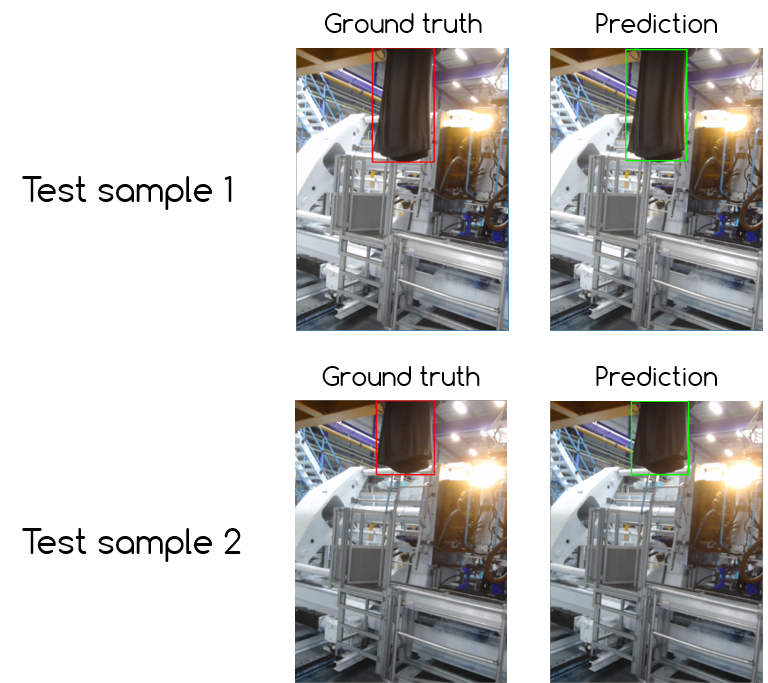
\includegraphics[scale=0.8]{images/chapter_3/parison_length_gt_prediction.png}}
\caption{Parison length inference example}
\label{fig:parison_inference}
\end{figure}
%
This system has been proven to be robust and to satisfy the identified industrial constraints. In particular, the system is reliable in term of prediction and it ensure real-time inference. Moreover, it does not need any expensive hardware. A simple RGB camera and a small computer allows for a cheap and non-intrusive solution which does not require any modification to the machine. 

With regard to our modelling approach we only care about the final parison. The parison length just before the molds closes for the blow-molding the final part. We made the assumption that the final length could provide enough information to explain the weight variability. INTRODUCE THAT THE CAMERA CAN BE USED TO A BETTER PROCESS CONTROL   

Since the final parts are produced in batches of one or two days, we built our own dataset using data from 5 different batches, corresponding to as many production days, for a total of 5597 samples and more than 5000 features. 

\section{Data processing TO BE FINISHED}

Some data processing operations on features are needed to reduce the overall feature space size. In fact, given the few individuals available in the dataset, a strategy of reducing the variables seems to be necessary in order to prevent the model overfitting and to improve its interpretability. In order to reduce the size of the input feature space we have applied to different approaches: an expertise-based and a statistical-based data processing.

\paragraph{Expertise-based data processing}

We relied on previous experts knowledge on the process to discard all features that cannot provide useful information for explaining the weight variability. For instance, all counter variables collected by the SCADA software do not bring any interesting information and can be removed. Moreover, the original feature space is composed of many timer variables, representing the time needed to execute a particular mechanical operation, which are redundant and provide no added value. Therefore, most of the timer variables have been removed from the dataset.


\paragraph{Statistical-based data processing}

Once the 

In order to reduce the number of features, three different statistical approaches have been used to select a subset of interesting features:
\begin{itemize}
    \item Feature selection using the  
    \item Feature selection using 
    \item Feature selection through \textit{Stability Selection} ADD REFERENCE TO CHAPTER 2.
\end{itemize}
%
A first approach to reduce the feature space was to remove the variables with too high correlations between them. Moreover, this operation allows us to avoid collinearity phenomena. Collinearity is the phenomenon in which correlation between predictor variables (or independent variables), such that they express a linear relationship in a regression model. When predictor variables in the same regression model are correlated, they cannot independently predict the value of the dependent variable. In other words, they explain some of the same variance in the dependent variable, which in turn reduces their statistical significance.

Moreover, in order to reduce multi-collinearity, we have deleted from the dataset some of the most highly correlated features. Finally, our dataset has a feature space of size 290. 



Data have been finally standardised to have zero-mean and unit-variance (See section ADD REF) . Standardising the features is not only important if we are comparing measurements that have different units, but it is also a general requirement for many machine learning algorithms.

Figure ADD REFERENCE resumes the  


% STABILITY SELECTION --> This section should be moved in chapter 2

% The rough idea behind stability selection is to inject more noise into the original problem by generating bootstrap samples of the data, and to use a base structure learning algorithm to find out which features are important in every sampled version of the data. For a feature to be considered stable (or important), it has to be selected in a high number of perturbed versions of the original problem. This tends to filter out features that are only weakly related to the target variables, because the additional noise introduced by the bootstrapping breaks that weak relationship.
% To make the above more precise, we have to dive into the mathematical details. The algorithm takes as input a grid of regularisation parameters $\Lambda$, and the number of sub-samples $N$ that need to be generated. Stability selection returns a selection probability $\Pi^{\lambda}_{k}$ for every value $\lambda \in \lambda$ and for every feature $k$, and the set of stable features $\hat{S}^{stable}\subseteq\{1,…,p\}$.

% The algorithm consists of two steps. In the sampling step the selection probabilities, or stability scores, are computed as follows. For each value $\lambda \in \Lambda$ do:

% \begin{itemize}
%     \item For each $i$ in $1,\dots, N$, do:
%     \begin{itemize}
%         \item Generate a boostrap sample of the original data $X^{n\times p}$ of size $n/2$.
%         \item Run the selection algorithm on the boostrap sample with regularisation parameter $\lambda$ to get the selection set $\hat{S}^{\lambda}_{i}$.
%     \end{itemize}
%     \item Given the selections sets from each sub-sample, calculate the empirical selection probability for each model component:
%     \begin{equation}
%         \hat{\Pi}^{\lambda}_{k} = \frac{1}{N}\sum_{i=1}^{N}
%     \end{equation}
% \end{itemize}

% In the scoring step we then compute the set of stable features according to the following definition

% \begin{equation}
%     \hat{S}^{stable} = \{k:\}
% \end{equation}

% where $\pi_{thr}$ is a predefined threshold. When the stability score for a variable exceeds the threshold $\pi_{thr}$ for one value in $\Lambda$, it is deemed stable.



\section{Exploratory data analysis TO BE FINISHED}


\subsection{Weight and Parison length}

A first work of data exploration has been done in order to study the correlation between the length of the parison just before the blow-molding phase and the weight of the blow-molded part. This was the first time that we had data available on the parison length. 

\subsection{Principal Component Analysis} \label{}

Since our feature space has a larger high size, it is quite complicated to to asses if there exist any hidden pattern within our data through a visual representation. However, it is possible to transform the input feature space in order to improve the interpretability of the input data. Principal Component Analysis (see section \ref{}) allows for a transformation of the original input feature space in a FINIRE. By applying the PCA it is possible to observe interesting information by only plotting the first principal components which account for the most of the variance of the input data. 
%
\begin{figure}
\centerline{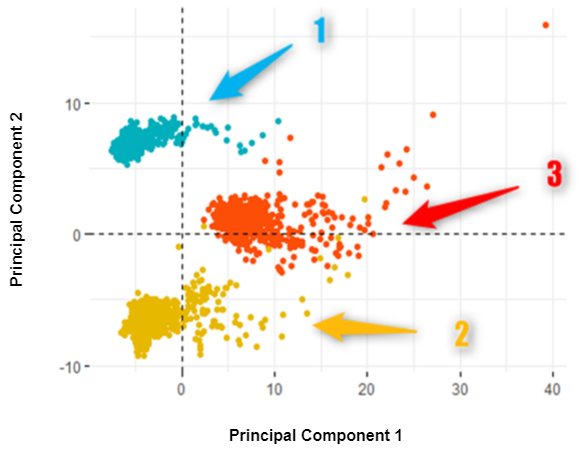
\includegraphics[scale=0.5]{images/chapter_3/PCA.png}}
\caption{Principal Components Analysis (sample projection on PC1 and PC2)}
\label{fig:pca}
\end{figure}
%
Figure \ref{fig:pca} shows the projection of the sample of only 3 batches on the first 2 principal components. This graphical representation allows us to identify two major information:
\begin{itemize}
    \item There exist some clusters
    \item For each cluster of data there exist a subset of points moving apart from the cluster.
\end{itemize}

A further analysis has allowed identify that each sample belonging to a specific cluster corresponds to a tank produced in a specific production day or batch. This imply that for the same tank reference, or model, the process data tend to be different depending on the production day. We will define this phenomenon as the ''Batch effect''. Moreover, the samples which moves apart from the centre of each clusters correspond to tanks produced in the first two hours after the machine has been started. This allows to identify two operating regimes: the \textit{transient} and the \textit{stable} regimes. 


\section{Supervised learning modelling}

Given our input processed data $P$ composed of $p$ process parameters and $n$ samples and the output vector $W \in \mathds{R}^{n}$ of the tank the role of the supervised learning modelling is to find the function $\hat{g}$ such that:
%
\begin{equation}
    \hat{g} = \argmin_{g \in \mathcal{G}} \sum_{i=1}^n (W_{i} - g(P_{i}))^{2} \enspace.
\end{equation}
%
We compared multiple regressive models: Linear Regression, Lasso Regression, Ridge Regression (see section \ref{Parametric models}), Random Forest and Gradient Boosting Tree (see section\ref{Tree-based methods}). The choice of relying on these algorithms is motivated by the following two reasons:
%
\begin{itemize}
    \item \textit{Interpretability}: Since we would like to understand what parameters affect the most the weight of the blow-molded tank, we are interesting in applying interpretable models. Linear models and Tree-based methods are easily interepretables.
    \item \textit{Performance}: These methods works quite well with structured data. When dealing with structured data, Deep Learning hardly overtakes traditional Machine Learning algorithms \citep{shwartz2021tabular}. 
\end{itemize}
%
In order to evaluate the predictive power of our models, we used two different approaches: cross-validation and batch cross-validation. 

\paragraph{Cross-validation}

In the basic Cross-validation approach, called \textit{K-fold} Cross-validation, the training set is split into $k$ smaller sets. The following procedure is followed for each of the $k$ “folds”:
%
\begin{itemize}
    \item A model is trained using $k - 1$ of the folds as training data
    \item the resulting model is validated on the remaining part of the data (i.e., it is used as a test set to compute a performance measure such as accuracy).
\end{itemize}
%
The performance measure reported by cross-validation is then the average of the values computed in the loop.
%
\begin{equation}
    CV_{K} = \frac{1}{K}\sum_{i=1}^{K}score_{i}
    \enspace.
\end{equation}
%
This approach can be computationally expensive, but does not waste too much data (as is the case when fixing an arbitrary validation set), which is a major advantage in problems where the number of samples is very small. In the context of our experimentation we have used a number of fold equal to 5.

\paragraph{Batch cross validation}

Instead of performing the cross-validation on $k$ randomly split folds of the training set, we decided to split the whole dataset in the different batches (production days) and to cross-validate the model on each batch. Since in our dataset we have 5 different batches, at each time, one batch is used as a test set and the remaining 4 batches are used to fit the model.

\begin{equation}
    CV_{batch} = \frac{1}{n\degree\;batches}\sum_{i=1}^{n\degree\;batches}score_{i}
    \enspace.
\end{equation}

The mean of the 5 different scores is calculated to have an accurate estimate of the model prediction performance. With this strategy we want to know if the model built on multiple batches is capable to fit data belonging to an unseen batch.  


\section{Results and Discussions} \label{Results and Discussions}

We used two different metrics: $R^2$ and the root mean squared error (RMSE). $R^2$, or coefficient of determination, is the proportion of the variance in the dependent variable that is predictable from the independent variable(s). Mathematically speaking, it can be expressed as follow:

\begin{equation}
    R^2 = 1 - \frac{RSS}{TSS}
    \enspace,
\end{equation}
where $RSS$ is the residual sum of squares and $TSS$ is the total sum of squares.
Values of the coefficient of determination range, normally, from zero (poor model) to one (perfect model) but can be negative if our model predicts our dependent variable worse than the mean of the independent variables. $RMSE$ is the square root of the $MSE$ and it has the advantage of explaining the average model prediction error in units of measure of the variable of interest. In our case, it provides the average error in prediction in kilograms. 

Both cross-validation and batch cross-validation return negative $R^2$ values for all the statistical models applied on our dataset. This highlight how the weight variability cannot be explained by our input process features. As it can be expected from looking at $R^2$, the RMSE score is far from being satisfactory regarding our needs. Results for Cross-Validation are resumed in table \ref{tab:cross_validation_results}.  

\begin{table}[]
\caption{Cross-Validation results}
\label{tab:cross_validation_results}
\begin{tabular}{lllll}
\toprule
\textbf{Algorithm} & \textbf{R² train} & \textbf{R² test} & \textbf{RMSE train} & \textbf{RMSE test} \\
\midrule
Linear Regression   & 0.72   &         &    &   \\ 
Lasso Regression    &        &         &    &   \\ 
Ridge Regression    &        & -0.26   &    &   \\ 
Random Forest       & 0.94   & -0.27   &    &   \\ 
Gradient Boosting   & 0.95   & -0.73   &    &   \\ 
\bottomrule
\end{tabular}
\end{table}


\begin{table}[]
\caption{Batch Cross-Validation results}
\label{tab:batch_cross_validation_results}
\begin{tabular}{lllll}
\toprule
\textbf{Algorithm} & \textbf{R² train} & \textbf{R² test} & \textbf{RMSE train} & \textbf{RMSE test} \\
\midrule
Linear Regression    &         &          &     &     \\ 
Lasso Regression     &         &          &     &     \\ 
Ridge Regression     &         & -0.26    &     &     \\ 
Random Forest        & 0.94    & -0.27    &     &     \\ 
Gradient Boosting    & 0.95    & -0.73    &     &     \\ 
\bottomrule
\end{tabular}
\end{table}

Both tables highlight how all the approaches tend to over-fit but struggle in generalise what has been learned on the train set to unseen new samples. This is especially true for Tree-Based methods that in general are more prone to over-fit. 

Results are quite astonishing but are showing evidence that it could be hard to apply statistical models in a field, manufacturing industry, where there is a lot of uncertainty. A further analysis has been conducted to try to explain and motivate these results. We have identified six possibles reason for these negative results:
%
\begin{enumerate}
    \item \textit{Non-stationarity of data}
    \item \textit{Lack of data characterising raw material properties}
    \item \textit{Low variability in product quality}
    \item \textit{Reliability of the input data}
    \item \textit{Weight too resultant}
\end{enumerate}
%
In the following paragraphs we will provide more details about each one of the identified sources of errors. 

\paragraph{Non-stationarity of data}

Results obtained with batch cross-validation have shown how our models do not generalise among different batches. Actually if we look at distributions of our input features we can see how they change considerably among different batches (Figure \ref{fig:Example of a process parameter variability in probability distribution}). 
%
\begin{figure}
\centerline{\includegraphics[scale=0.4]{images/chapter_3/process_parameter.eps}}
\caption{Example of a process parameter variability in probability distribution}
\label{fig:Example of a process parameter variability in probability distribution}
\end{figure}
%
A “Two-sample Kolmogorov-Smirnov” test has been applied on all two-pair batch combinations. Looking at results, only 35\% of the input features share the same probability distribution over all batches, with a $0.95$ confidence level.
In order to correct apply Machine Learning models the stationarity hypothesis must be verified. In fact, a trained model expects that any new input sample follows the same distribution of the data used to train the model. 

\paragraph{Lack of data characterising raw material properties}

The change in data distribution could may be the consequence of some external events or factors that we do not control and do not take into account within our own input process data. We claims that ''batch effect'' we observe in the data could be a consequence of certain changes in rheological properties of raw materials. In fact, the final part is the result of the transformation of raw material through our complex process. Unfortunately, to this date, these data are not available and they cannot be integrated in our dataset. Further studied have been carried out in order to understand if it is possible to measure in real-time some rheological properties of the material. There exist some industrial online rheological systems which provide continuous measurements of the melt flow rate or apparent viscosity directly on the manufacturing process. Unfortunately, the cost of this solution is not economically viable, especially considering that such a system would have to be installed for each of the 6 screws.

\paragraph{Low variability in product quality}

The manufacturing process taken into account already has a good performance in term of capability. The variability of the in term of quality does not change too much. The scrap rate is under 3\% and the tolerances limits set to evaluate the compliance of blow-molded tank are quite strict. In general, we look for a weigh variability of about 300 grams which corresponds, for a tank with an average weight of $8.5$ kilograms, to about $3.5\%$ of the total weight. The problem would have been simpler with higher weight variation.     

\paragraph{Reliability of the input data}

As we look for small variations in term of weight, it is important that the input data are accurate enough to provide all the information needed to explain the small quality variability. In an industrial environment, such as a production plant, the collected data are most of the time noisy. The maintenance of the sensors cannot be done regularly. As a consequence, some sensors may provide values which do not corresponds to the reality of what is going on. Moreover, the SCADA software computes some aggregate operation on the input time series-data, which can lead to a lost of information. Finally, it is quite complex to attach the extrusion data to the traceability serial number of a tank since Extrusion is a continuous process and there are not precise triggers to define what data belongs to a part or to another one. The way the extrusion data are attached to a manufactured part could lead to a certain uncertainty.  


\paragraph{Weight too resultant}

Another possible explanation is directly related to the nature of the output variable considered in our problem, the weight. In fact, the weight is a resulting variable which depends on the distribution of the material on the tank surface. However, different material distributions can produce the same final weight. In others words, different manufacturing conditions, represented by different process parameters values can lead to the same weight. As a consequence, the model struggles to learn the function which approximate the relationship between process parameters and quality data.

These results highlights the difficulties we can encounter when dealing with manufacturing process data. However, in the following section we will show how the work presented in this chapter has made it possible to start a new project in the company to improve the manufacturing process. 


\section{SmartBMM: towards smarter machines}

The data analysis results presented all along this chapter have shown the inability to explain the tank weight variability given the blow-molding process data that are considered as critical by the process experts. The possible reasons have been discussed in detail in the previous section. What the analysis has also highlighted is that the most of the scraps occurs just after the machine start-ups (see section \ref{}). As shown previously, right after the machine start-up, the extrusion blow-molding process is not completely stable which increase the overall scrap rate of the blow-molded parts. Moreover, an interview of different extrusion blow-molding experts has highlighted that there are not common and shared best practices to start the machine. As a consequence there, is a lot of variability between startups.
%
\begin{figure}
\centerline{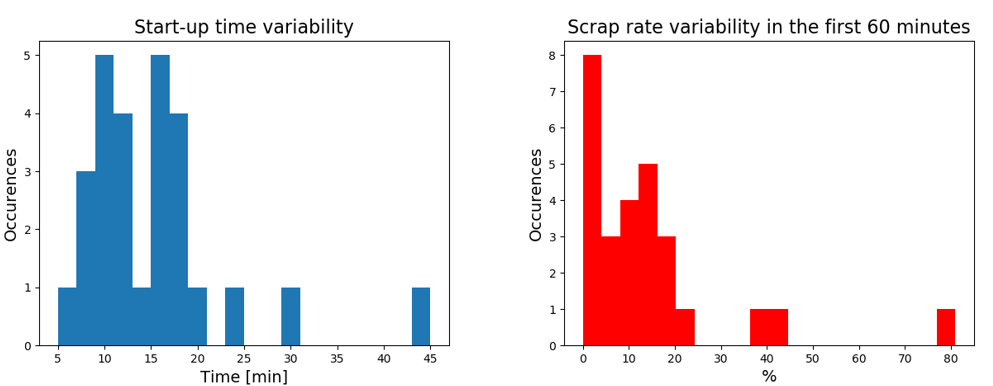
\includegraphics[scale=0.7]{images/chapter_3/smartbmm_barchart.png}}
\caption{Time and scrap rate variability for 27 machine start-ups in a Plastic Omnium plant}
\label{fig:smartbmm_barchart}
\end{figure}
%
In Figure \ref{fig:smartbmm_barchart}, an example of the previously described variability for 27 machine start-ups performed in a Plastic Omnium plant. On the left bar-chart, we can see how the time needed to start the machine may change from a start-up to another. Sometimes the start is done in 10 minutes, other times a full start may take around 15-20 minutes. There are also three occurrences for which the start-up took more than 20 minutes. In the same way, the right bar-chart highlights how the scrap rate in the first 60 minutes may change from a start up to another. Most of the time, hopefully, the scrap rate does not exceed the 5\%, but there are many starting for which the scrape rate value is above 10\% which is huge. Starting from these observations, it seemed necessary to us to put some efforts in trying to improve the way the Extrusion Blow-Molded machines are started. In particular, we claims that by automating and by optimising the machine start-up we could be able to reduce the uncertainty introduced by the human way of starting the machine. This would allow for a faster convergence towards the stable regime of the machine and, as a consequence, to a smaller number of part non-conformities.   

We are aware the scraps may have a multitude of reasons which do not depends on the way the machine is started, but we claims that providing repeatable and optimised starting should benefit at the overall performance of the manufacturing process. 
The project was initially conceived to handle just the machine starting but it has been, later on, extended to also cover the Purge cycles of the machine. The reason is quite obvious, by ensuring good Purge cycles we can reduce the risk of incurring in contamination/inclusion problems. In this context, we have developed the \textit{SmartBMM} solution. \textit{SmartBMM} is a software which leverages the real-time data collected directly from the PLC of the machine and the past data to elaborate the best instructions to get the machine started without any manual intervention of the operators.

\begin{figure}
\centerline{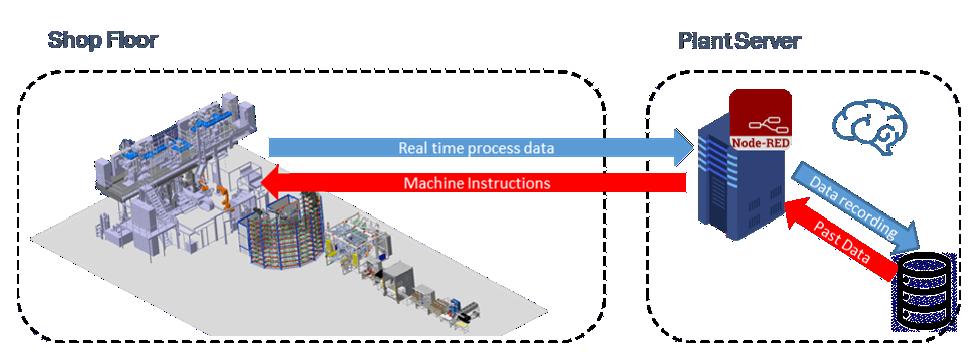
\includegraphics[scale=1]{images/chapter_3/SmartBMM.eps}}
\caption{\textit{SmartBMM} software}
\label{fig:SmartBMM}
\end{figure}

Figure \ref{fig:SmartBMM} shows broadly how the SmartBMM works. The SmartBMM software collects real time data directly from the PLC and store it in a database in order to be able to retrieve it later. When the SmartBMM software is started the data collection continue, but, this time, the machine starts to write information to the PLC to execute a set of operations. The software takes the real time incoming data and the past data to elaborate the machine instructions to get the machine to the production conditions. The stored data are used to compute the production extruder speeds which, accordingly to past data, minimise the non-conformities rate. Looking at previous production runs we are able to retrieve the process conditions which leads to a better performance and a lower scrap rate. The software is developed using the \textit{Node-RED} \citep{nodered} programming tool. Node-red is a low-code programming for event-driven applications which has been specifically designed to work with IoT and that allows easy interfacing with machines through different communication protocols.

Instead of manually start the machine by pressing simultaneously multiple buttons on the HMI (Human Machine Interface), machine setters and operators have to press only one button to start a cycle, whether it is a \textit{Starting} cycle or a \textit{Purge} cycle.  

\begin{itemize}
    \item The starting functionalities leverages the real-time data collected directly from the PLC of the machine and the past data to elaborate the best instructions to get the machine started without any manual intervention of the machine operators. The set of consecutive instructions provided to the machine are fairly standard. The extruders are started, then the material is fed into the screw, than the extruder speed is raised ans so on. However, our system does not rely on timers to trigger the machine instructions. In real time the process status is controlled and the next machine instruction is triggered only if the process meets all requirements.
    Two starting functionalities are available: \textit{Full} and \textit{Downtime}. The Full executes a starting when the machine is completely stopped. The Downtime functionality, on the other hand, go back to production condition when the machine has been temporarily stopped.
    %  There exist two Purge cycles: the \textit{Purge Out} and the \textit{Purge In}. The Purge Out cycle is done when the machine is stopped for more than 2 hours to remove any FINIRE. The Purge In is done every time that the Purge Out has been done to prepare the extruder for the production run. 
    \item The Purge functionalities allow to improve the Purge cycles of the machine.
    During the Purge cycles we want to ensure that enough material transit into the extruders at high pressure to clean them of material residues. Instead of relying on fixed speed values or timer, we have developed a \textit{PID controller} which regulates the extruder speeds to ensure to be constantly above the pressures targets. Moreover, the amount of material transiting inside screw is controlled in real-time. This allows to finish the Purge cycle only when the exact amount of material is transited inside the screw.     
\end{itemize}
%
By taking advantage of Starting and Purge functionalities, we aim to reduce either the "weight not OK" and the "contamination" scraps, which account for $2/3$ of the total amount of non-conformities.

The functionality is chosen by the operator through a graphical user interface (GUI) specifically developed to allow an easy interaction with the software (Figure \ref{fig:SmartBMM_gui}).
%
\begin{figure}
\centerline{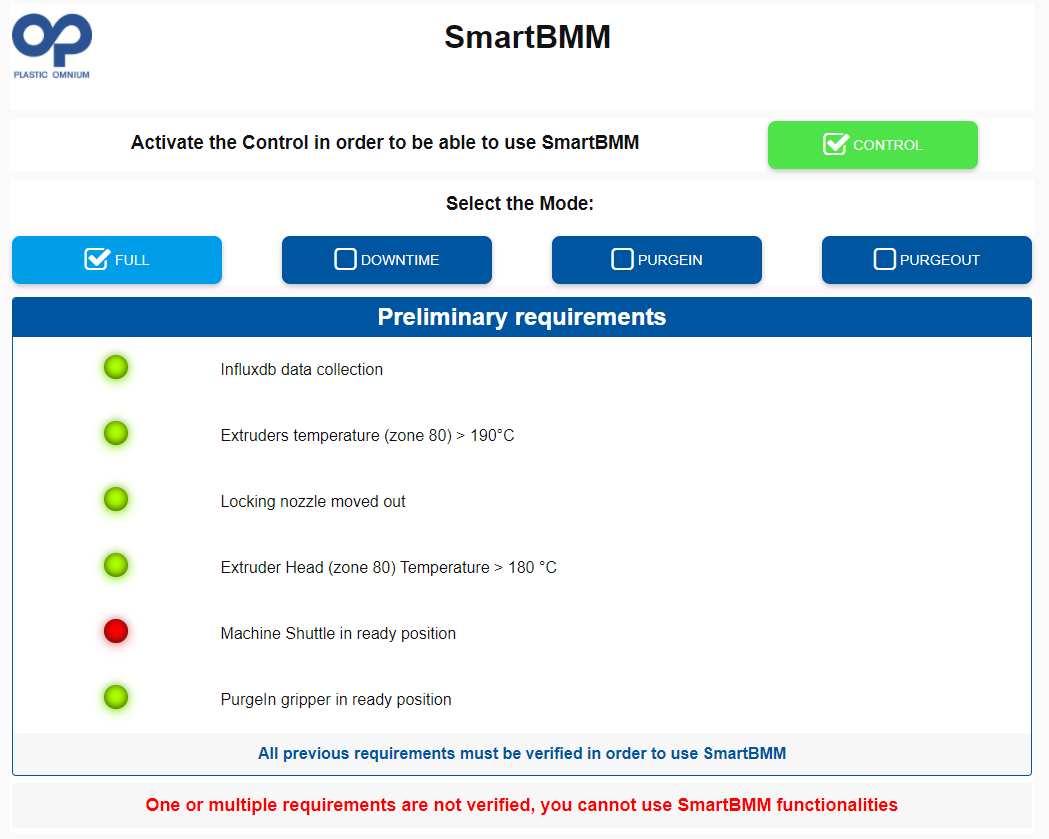
\includegraphics[scale=0.5]{images/chapter_3/SmartBMM_gui.png}}
\caption{\textit{SmartBMM} GUI}
\label{fig:SmartBMM_gui}
\end{figure}
%
An interesting element of this project, is the way we have decided to pilot the machine. In fact, the logic that allows to perform the machine cycles is developed outside of the machine PLC. Historically, all manufacturing processes, including Extrusion Blow-Molding, rely in PLC programs to execute the set of instructions to allow the manufacturing machine to work correctly and to allow for the transformation of the raw materials to the finished product. The choice of developing our solution outside the PLC is motivated by the following reasons:
%
\begin{itemize}
    \item PLCs are very robust and safe, but they lack in flexibility. PLCs are conceived to execute a row a set of logical instructions but they do not lend themselves well to be used concurrently with other systems such as databases. Developing a more complex logic which involves the data storage and the communication with databases is by far more easy to do using traditional software development tools, compared to the PLC.
    \item Implementing the logic on an external system such as a physical or a virtual server reduce the number of PLC modifications of the machine. Our software is something non-intrusive which can be installed remotely on a server without any direct modification of the PLC program. It is something that can be plugged to the machine to introduce new functionalities. This makes it possible to reduce costs considerably, since it is not required to directly modify the PLC program which may require the intervention of an external consultant.
\end{itemize}
%
This strategy has, however, a main drawback. Our tools completely rely on the plant network to communicate the instructions to the PLC. Which means that a bad network could be a bottleneck for the correct functioning of our software. Security features have been added on the software side to interrupt the communication with the machine if any network failures prevents to communicate with the machine.

In our opinion this is an example of a cyber-physical system. SmartBMM leverages the sensor networks with data processing to monitor and control the physical environment, with feedback loops able to elaborate the best set of machine given the different process conditions.


\section{Conclusion}

In this chapter, we have presented an empirical evaluation of our approach involving the industrial context in which this research work has been carried out. The results highlighted the impossibility to predict the tank weight using the data currently collected through the home made \textit{SCADA system} and enriched by the parison length measurement. Results are unexpected but are showing evidence that it could be hard to apply statistical models in a field, manufacturing industry, where there is a lot of uncertainty and where it is not possible to take into account all those elements that contribute to the variability of the part quality. Possible explanations of these results have been discussed. However, this research work has nevertheless made it possible to identify some room for improvement of the Blow-Molding process. In particular, the exploratory data analysis has shown how most of the part non-conformities occurs just after the machine start-ups where the process is not yet stable. This made it possible to start the \textit{SmartBMM} project.  


\subsection{Scientific Contribution}

On the scientific point of view, the results presented in this chapter allows to questioning the effectiveness of data-driven methods in the context of the manufacturing industry. Data-driven methods have been proven to be effectiveness in many applications but in order to work well it is necessary to have data that respects some quality constraints. The results obtained in this chapter have shown that applying such an approach on all the data available and pretending to obtain good results is trivial. The approach of taking many input data and feed them into a generic AI data-driven model could not work in an environment where there is a lot of uncertainty. Instead of working directly with all the data available, a complex problem should be broken down in many sub problems where data quality is properly controlled. As we will present in the following chapter, by breaking down the problem in sub-parts and by mastering the data it is possible to obtain interesting results. 

\subsection{Industrial Contribution}

This chapter has three main industrial contributions.
\begin{itemize}
    \item Firstly, the work presented in this chapter has made it possible to call into question certain beliefs about the functioning of the blow-molding process. The critical process parameters considered as critical to ensure the correct functioning of the process do not allow to explain the tank weight variability. The control limits previously set for the critical parameters of the process, for ensuring the correct functioning of the production process, have proved to be insufficient to explain the tank weight variability.
    \item The Parison length measurement has opened new research perspectives. By measuring in real-time the length of the Parison, we will eventually be able to ensure the correct material distribution over the overall parison length. By ensuring the correct material distribution and by controlling the parison length we should be able to improve the process stability and, as a consequence, the quality of the manufactured parts. Further information and perspectives will be presented in chapter \ref{Contributions and perspectives}.
    \item Finally, the \textit{SmartBMM} software that has been developed starting from the results obtained trough the data analysis process, has made it possible to improve the machine start-ups phases which are responsible for those transitional phases that lead to an higher scrape rate. By ensuring a faster and better start-up, we have proven to be able to shorten the duration of this transitional phase. By reducing the duration of the transitional phase it is possible to indirectly reduce the percentage of parts that do not comply with quality standards. Future works will make use of the parison length measured through the use of the camera to add to SmartBMM new functionalities.  
\end{itemize}



% Chapter 4
\setcounter{mtc}{7}
\chapter{Thickness inference using thermal imaging} \label{Thickness inference using thermal imaging}
\minitoc


\section{Introduction}

In the previous chapter, we showed the difficulty of inferring the weight of the tank given the process parameters as they are collected today. The possible explanations have been addressed in section \ref{Results and Discussions}. The weight is a quality indicator that summarises the information about the overall amount of material which composes the fuel tank. However, as we saw earlier, the weight does not guarantee the correct distribution of the material over the whole surface, as different thickness distributions may lead to the same weight. As a consequence, we decided to focus directly on thicknesses, which provide more accurate information about the distribution of the material over the surface. Of course, measuring the tank thicknesses using the only the available process parameters could be challenging as we have no information about the geometry of the tank. It is therefore necessary to collect new data that can provide us with spatial information.

In this chapter, we propose a new approach to perform a real-time, non-destructive quality control to measure thicknesses of blow-moulded parts. The proposed approach makes use of deep learning data-driven methods to leverage the thermal inertia of the manufactured plastic part, captured through thermal imaging, to infer the thicknesses of the part surface without any direct measurement. Compared to traditional quality inspection approaches, which aims to detect visual defects of manufactured products, our approach leverages thermal information to perform a non-visual quality control. The first experimental results on real industrial data are very promising and demonstrate that the proposed method could achieve satisfactory performance in industrial conditions.

\section{Weight and thicknesses}

Before digging into the details of the proposed approach, it is interesting to explore the relationship between the thickness values and the tank weight. In order to asses if there exist a measurable statistical relationship between the weight and the tank thickness a simple correlation analysis has been conducted. By taking advantage of 300 measured tanks, for which the weight, as well as the thickness of a limited number of critical points, the correlation between each thickness-weight pair is computed. Figure \ref{fig:thickness_points} shows the coordinates of the six points for which the thickness was measured. 
%
\begin{figure}
\centering
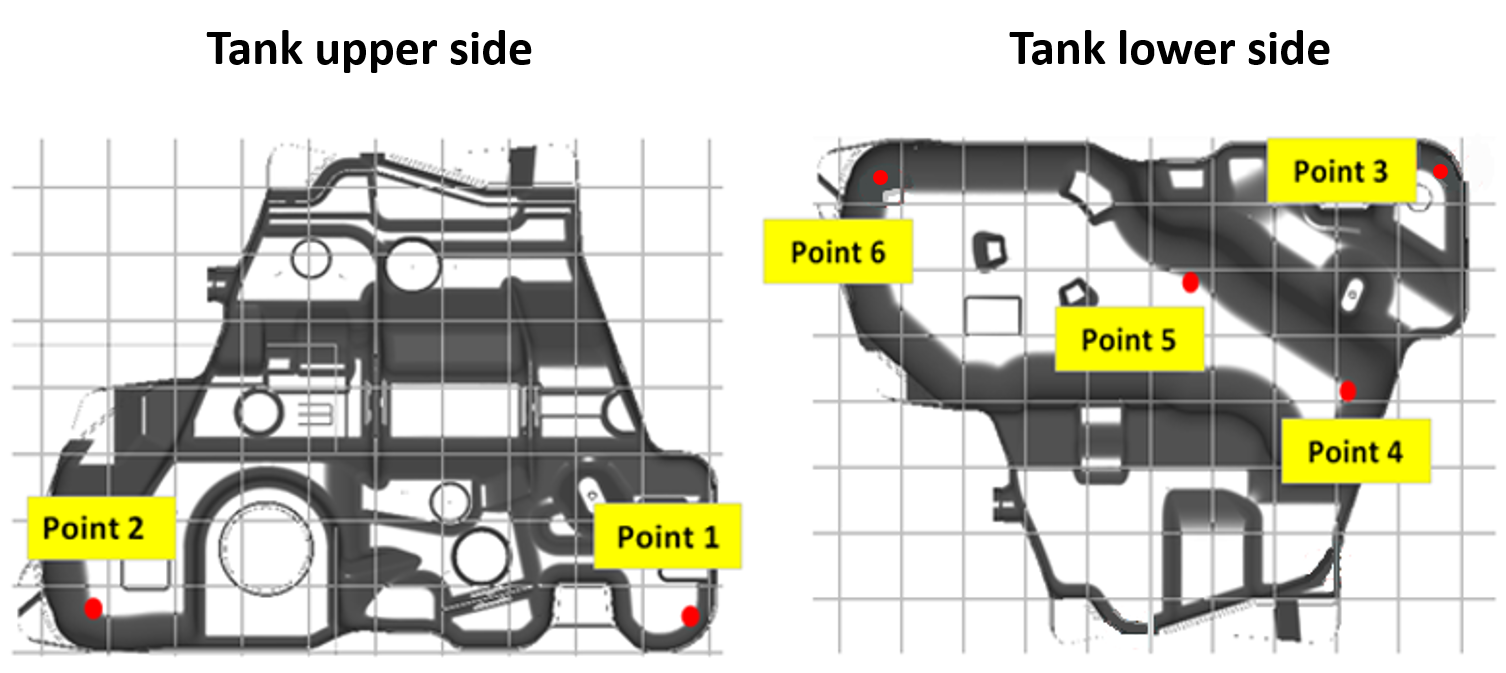
\includegraphics[scale=0.55]{images/chapter_4/Thickness_points.png}
\caption{Thickness points}
\label{fig:thickness_points}
\end{figure}
%
Figure \ref{fig:thicknesses_weight_scatter} shows the scatter plots drawn by plotting each thickness-weight pair, with one variable on each axis. For each plot, the regression line is drawn to visualise the trend. As visible in the Figure, there exist a minor correlation between some of the thickness points and the tank weight. The highest correlation, between the thickness at point 5 and the weight, is 0.40: there is a lot of dispersion within data, and a higher weight does not mean a higher thickness. This confirms our assumption that it is impossible to ensure the correct distribution of material over the surface of the tank by monitoring solely the weight. 
%
\begin{figure}
\centering
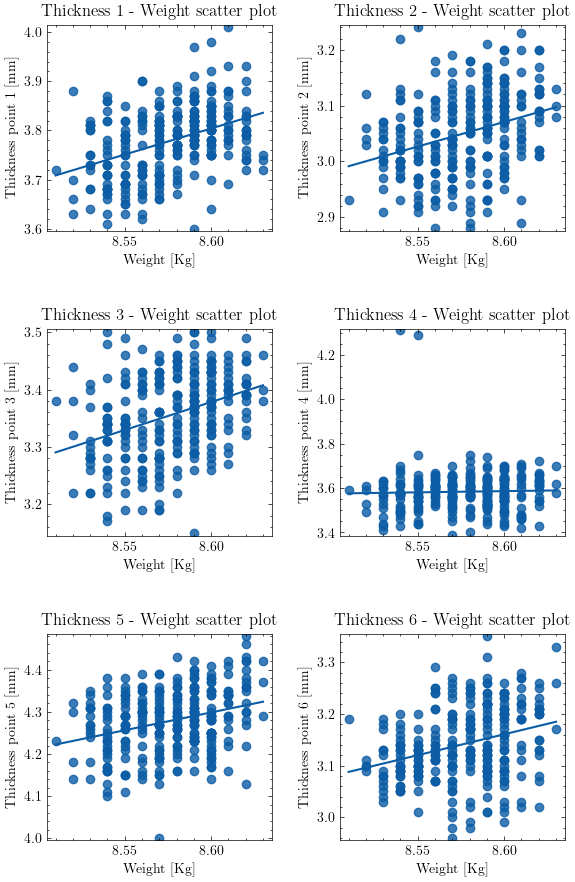
\includegraphics[scale=0.9]{images/chapter_4/thickness_weight.png}
\caption{Thicknesses - weight scatter plots}
\label{fig:thicknesses_weight_scatter}
\end{figure}
%
The weight and the sum of the 6 measured thicknesses are slightly more correlated (Figure \ref{fig:thickness_sum_weight_correlation}) as expected since the weight is proportional to the amount of material composing the fuel tank.
%
\begin{figure}
\centering
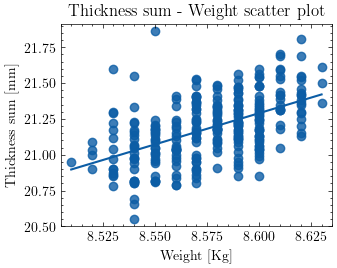
\includegraphics[scale=1]{images/chapter_4/thickness_sum_weight.png}
\caption{Thickness sum - Weight correlation}
\label{fig:thickness_sum_weight_correlation}
\end{figure}
%
Results presented in this section show that the weight of the tank is not sufficient to ensure the correct distribution of the material along the surface. In order to improve quality control and ensure that thicknesses meet customer specifications it is advisable to focus our research work directly towards the inference of thicknesses.

\section{Motivation} \label{Motivation}

Our work is motivated by the empirical observation of the cooling of blow-moulded parts in the first minutes after blowing. Areas of the parts have different cooling behaviours depending on their thickness. 

Areas with smaller thicknesses cool down faster than those with higher thicknesses. For the thicker zones, the surface temperature even starts to increase before decreasing (Figure~\ref{fig:temperature_cooling}).
%
\begin{figure}
\centering
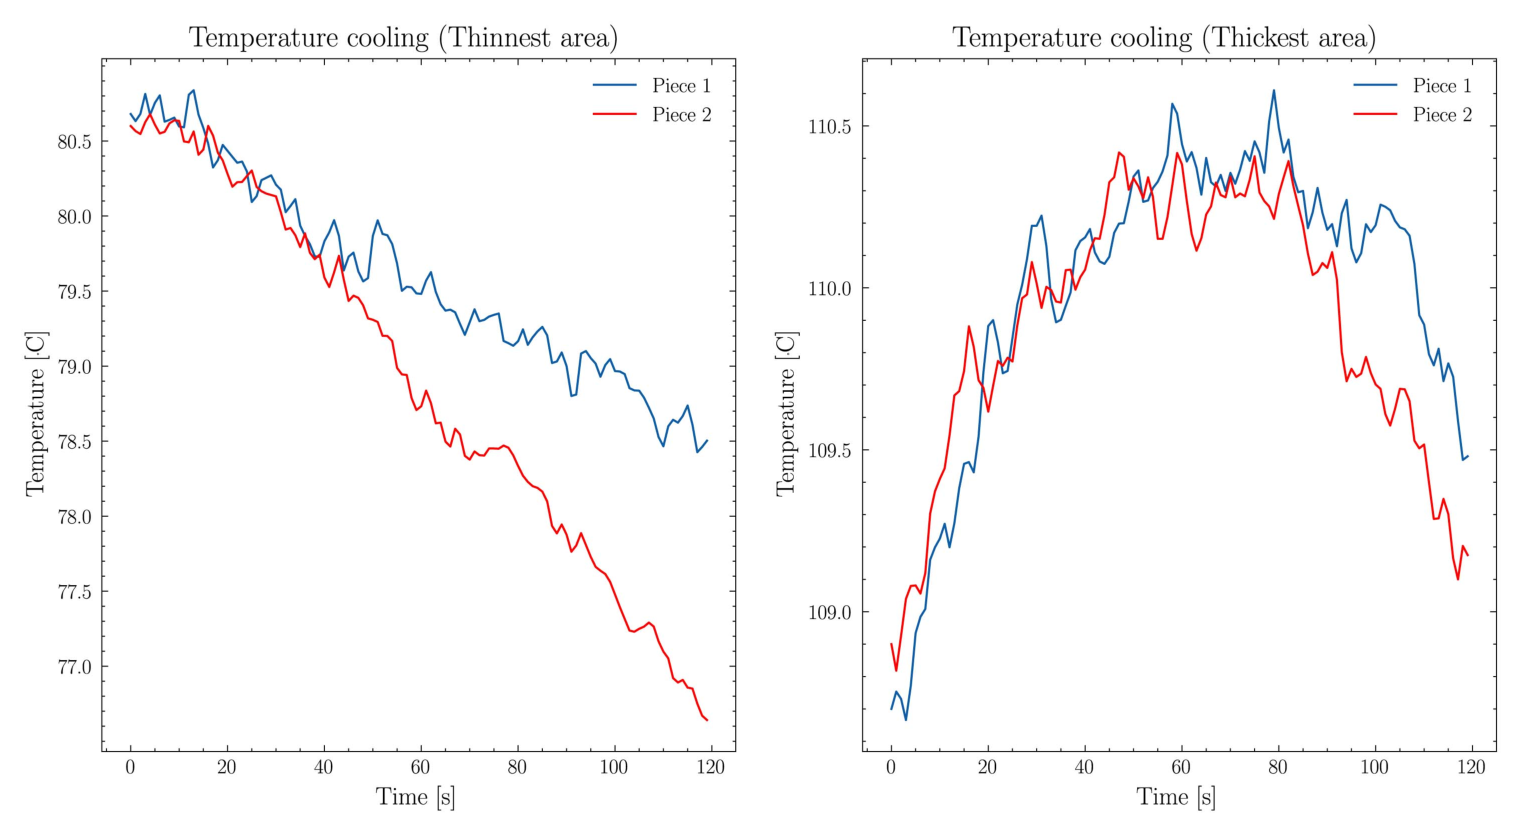
\includegraphics[scale=0.55]{images/chapter_4/cooling.eps}
\caption{Surface temperature cooling profiles at the thinnest (left) and thickest (right) areas of the blow-moulded part}
\label{fig:temperature_cooling}
\end{figure}
%
This phenomenon is due to the release of energy from the innermost plastic layer that has not be in direct contact with the mould surfaces.
As presented in Section \ref{The key quality characteristics of a blow-moulded fuel tank}, this surface temperature decay, easily measured by thermal imaging, could be leveraged to infer the thickness of the part.  
In particular, we make two assumptions:
\begin{itemize}
   \item The cooling conditions of the environment where the part is monitored are the same for all parts produced. Therefore, we consider that the variations of the temperature of the production area are negligible.
   \item The physical and chemical properties of the material are assumed to be constant over the entire surface of the part. In particular, the thermal and infrared transmittances of the material should be approximately constant.
\end{itemize}

Based on these assumptions, we designed three data-driven methods to model the relationship between the surface temperature variations of critical areas of the part and the corresponding thickness values. The first approach, by one-dimensional time series, exploits the cooling dynamics, one point of the part at a time, whereas the second method processes the part globally, taking into account unity of part (points belonging to the same part are processed simultaneously) and spatial information (points are positioned on the part surface).

\section{Proposed methods}

In this section, we present new approaches to predict the thickness of blow-moulded parts. We propose a non-intrusive real-time thickness inference exploiting the variations of surface temperatures over time on different areas of the blow-moulded part. 
Unlike traditional thickness quality control methods, our system is able to predict thickness values at critical points of the part within minutes, allowing real-time operation.

Three different approaches to model the temperature-thickness relationship are proposed:
%
\begin{itemize}
    \item \textit{Parametric temporal approach}: The Parametric temporal approach involves the use of a parametric function to approximate the pointwise temperature surface decay. The function parameters, retrieved through curve fitting, may then be used as input features for a machine learning regressor.
    \item \textit{Flexible temporal approach}: The flexible temporal approach, as the parametric temporal one, takes advantage of the pixel-wise temperature decay. Instead of compressing the information through the use of a parametric function, the flexible temporal approach leverages the ability of deep learning to extract meaningful features from raw signals.
    \item \textit{Spatio-temporal approach}: The spatio-temporal approach leverages not only the temporal temperature information, but also the spatial one. Instead of extracting the temperature time series for each critical point of the blow-moulded parts we can design an \textit{end-to-end} deep learning architecture able to directly handle the input thermal video. In such a way, we should be able to take into account the tank unit intrinsic information which is completely lost in the previous approaches.
\end{itemize}
%
These three approaches are presented in more detail below.

\subsection{Parametric temporal approach} \label{Parametric Temporal approach}

The first approach consists of three phases: time series extraction, time series approximation by parametric curve fitting and thickness prediction using the parameters of the approximated temperature surface decay.

\paragraph{Time series extraction:} 

The time series extraction phase aims to process the input thermal video in order to retrieve the temperature time series of a limited number of critical points, for which the thickness value is known. These time series constitute the input data of our data-driven model. Given $K$ critical points of each part for which the thickness values are known, and given the thermal video $X_{i}$, we are interested in extracting the time series ${x}_{ik} = \left (X_{i}(\xi_{k}, \zeta_{k},1),\ldots,X_{i}(\xi_{k}, \zeta_{k},T) \right) \in \mathds{R}^{T}$, with $T$ time steps, where $(\xi_{k}, \zeta_{k}) \in \{1,\ldots,h\}\times\{1,\ldots,w\}$ indexes the pixel matched to key point $k \in \{1,\ldots,K\}$. For a set of $n$ input thermal videos, this first phase produces a dataset
\begin{equation}
    D = \left\{\{x_{ik},y_{ik}\}_{k=1}^K\right\}_{i=1}^n
\end{equation}
of $K \times n$ pairs $(x_{ik},y_{ik})$ where $x_{ik} \in \mathds{R}^{T}$ is the time series corresponding to key point $k$ in thermal video $i$ and $y_{ik} = Y_{i}(\xi_{k}, \zeta_{k}) \in \mathds{R}$ is the corresponding thickness value.


\paragraph{Time series approximation:}

In order to reduce the number of input features we approximate the surface-temperature decay time series by a parametric expansion,  to compress the temporal information into a limited number of new features, corresponding to the parameters of the function. Temperature-surface time series have a fairly simple shape (Figure \ref{fig:temperature_cooling}). The predominantly parabolic shape of the time series lends itself well to be approximated with simple functions, with few parameters. We compared the following three parametric models:
\begin{itemize}
    \item Power Law: $y=ax^b$,
    \item Polynomial (2nd degree): $y=ax^2+bx+c$,
    \item Logarithmic: $y=a+b\log(x)$.
\end{itemize}

In such a way, the different cooling behaviour, observable in different areas of the part could be expressed through a limited number of new parameters. Moreover, the functional approximation smooths the time signal, thereby filtering the measurement noise. The new features may be then used as the input data for a regression model.
Mathematically speaking, the time series approximation produces a new dataset,
%
\begin{equation}
    D = \left\{\{z_{ik},y_{ik}\}_{k=1}^K\right\}_{i=1}^n
    \enspace,
\end{equation}
%
composed of $K\times n$ pairs $(z_{ik},y_{ik})$ collection pairs where ${z}_{ik} \in \mathds{R}^{P}$ are the $P$ parameters obtained by fitting the parametric function to the time series $x_{ik}$.

\begin{sidewaysfigure}
\centering
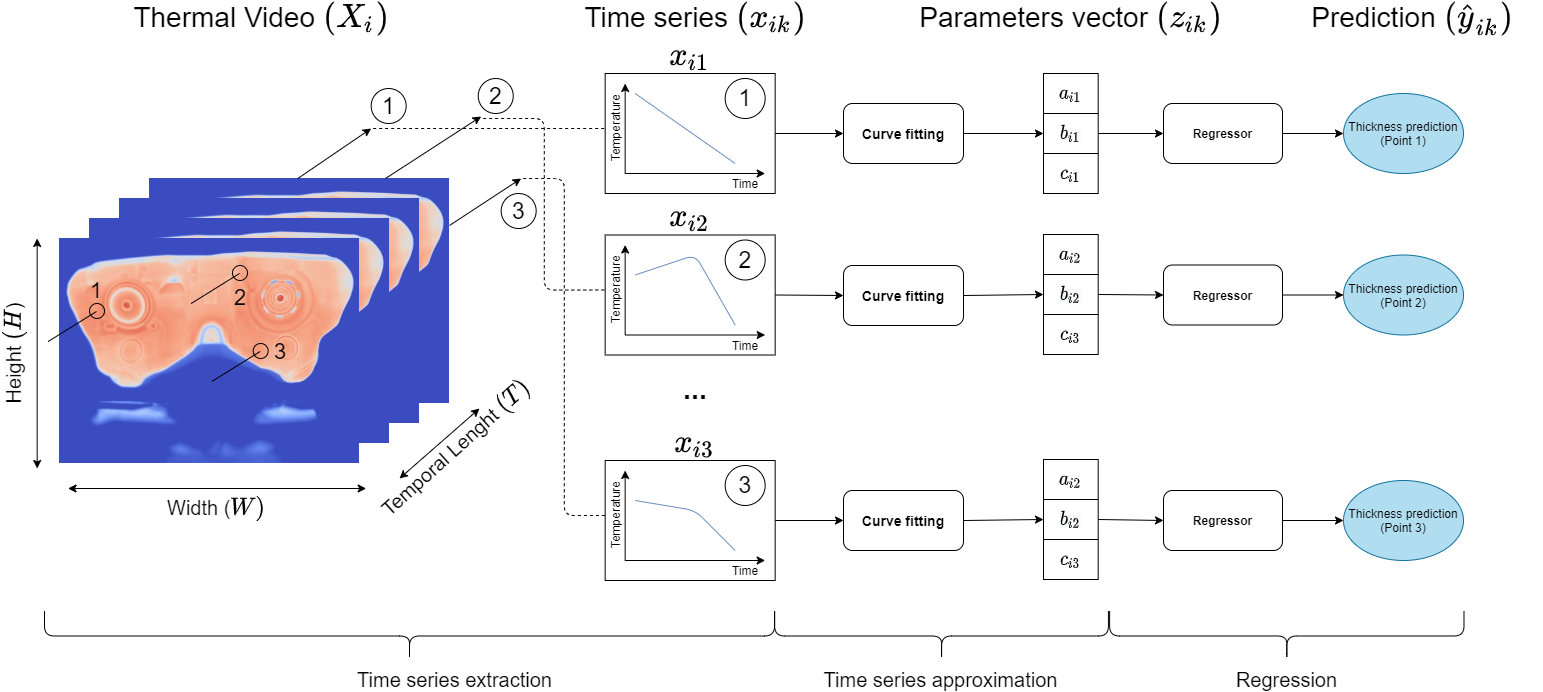
\includegraphics[scale=0.4]{images/chapter_4/Parametric_Temporal.png}
\caption{Parametric temporal approach}
\label{fig:parametric_temporal_approach}
\end{sidewaysfigure}

\paragraph{Time series regression:}
Any machine learning method can then be applied to predict the thickness value of a given key point based on the parameters computed by fitting the surface-temperature time series.  The role of the machine learning algorithm is to estimate a function $\hat{g}$ such that
\begin{equation}
    \hat{g} = \argmin_{g \in \mathcal{G}} \sum_{i=1}^n \sum_{k=1}^K (y_{ik} - g(z_{ik}))^2 \enspace.
\end{equation}


\subsection{Flexible temporal approach}

As illustrated in Figure \ref{fig:temporal_approach}, the proposed method consists of two phases: extraction of the time series and thickness value regression through a recurrent neural network (RNN). The time series extraction is carried out exactly in the same way as for the parametric temporal approach (see Section \ref{Parametric Temporal approach}).  

\begin{sidewaysfigure}
\centering
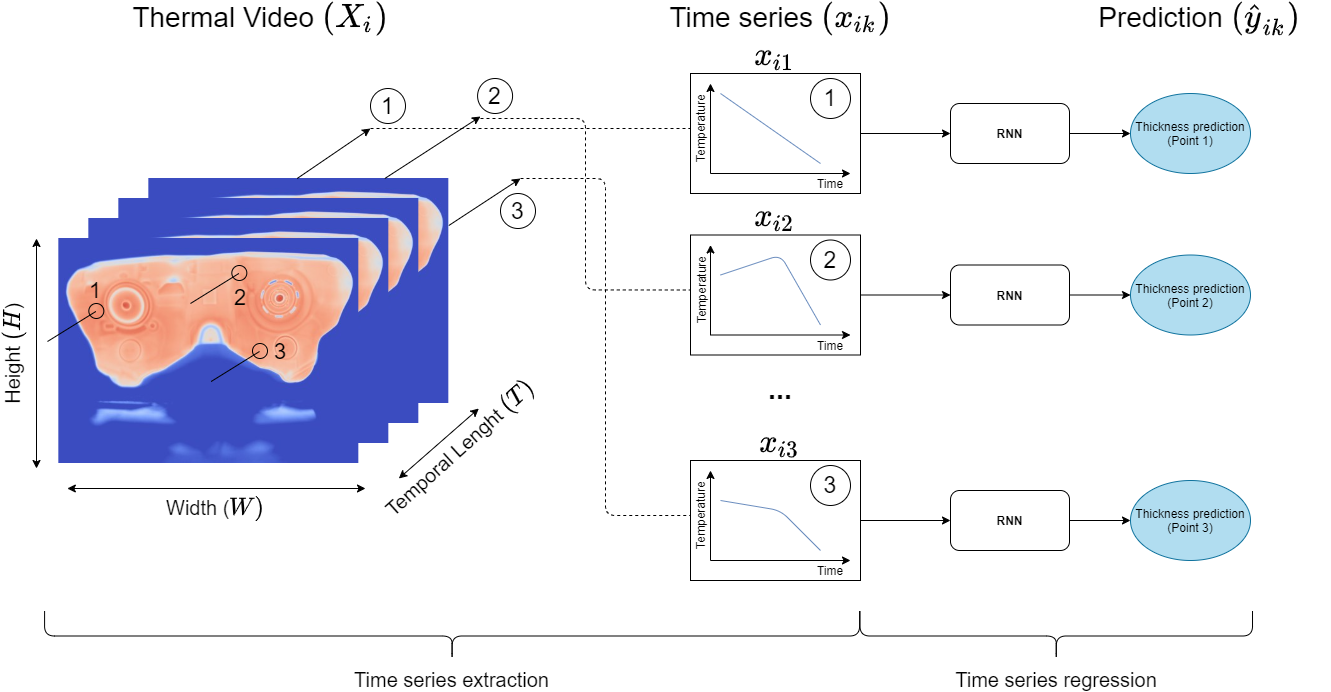
\includegraphics[scale=0.4]{images/chapter_4/Flexible_Temporal.png}
\caption{Flexible temporal approach}
\label{fig:temporal_approach}
\end{sidewaysfigure}

\paragraph{Time series regression:}

Given the extracted time series and the corresponding thickness values, our problem can be formulated as a supervised machine learning problem, more specifically, as a univariate time series regression problem. With univariate time series regression we mean the task of predicting the real number value of the dependent variable, the thickness, given a single dependent variable corresponding to a sequence of discrete-time data. Formally, we look for function $\hat{g}$ such that
\begin{equation}
    \hat{g} = \argmin_{g\in\mathcal{G}} \sum_{i=1}^n \sum_{k=1}^K (y_{ik} - g(x_{ik}))^2 \enspace.
\end{equation}
%
As our hypothesis is that temporal information plays a key role in thickness discrimination, we chose to use a recurrent neural network (see Section \ref{Recurrent Neural Network}) to model the dependency. 
%
\begin{figure}
\centering
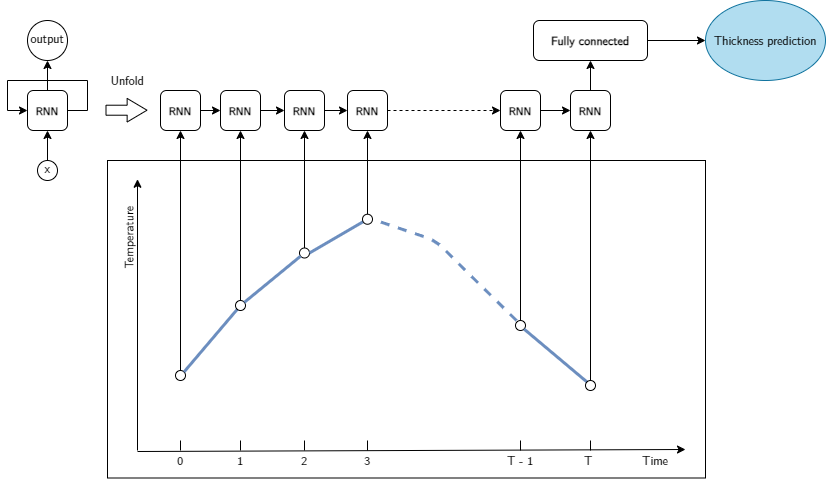
\includegraphics[scale=0.45]{images/chapter_4/rnn_model.png}
\caption{RNN-based model}
\label{fig:rnn_model}
\end{figure}
%
Inspired by the results achieved by RNNs in the domain of sequential data, we designed a simple RNN to address our problem (Figure \ref{fig:rnn_model}). The main idea behind our pipeline is to sequentially process the temperature at each time step $t$ by taking into account information from prior inputs to predict the current input and output. The last output computed by the RNN model is then passed through a fully connected layer to produce a scalar output aiming at approximating the thickness of the part area for which the time series has been extracted.

\subsection{Spatio-temporal approach} \label{Spatio-temporal approach}

Compared to the previous approaches, the method proposed in this section aims to leverage not only the temporal temperature information, but also the intrinsic information of the tank unit. Instead of extracting the temperature time series for each critical point of the blow-moulded parts we design an \textit{end-to-end} deep learning architecture capable of directly processing thermal video as input data. In this setup, the dataset
\begin{equation}
    D = \{(X_{i}, Y_{i})\}_{i=1}^{n},
\end{equation}
is a collection of pairs $(X_{i}, Y_{i})$ where $X_{i} \in \mathds{R}^{h \times w \times T}$ is the input thermal video made of $T$ frames of height $h$ and width $w$, and $Y_{i} \in \mathds{R}^{h \times w}$ is the corresponding thickness image, that is, the 2D array of thicknesses on each of the input pixels. The role of the spatio-temporal approach is to estimate a function $\hat{g}$ such that
\begin{equation}
    \hat{g} = \argmin_{g\in\mathcal{G}} \sum_{i=1}^n \left( Y_{i} - g(X_{i})\right)^2 \enspace,
\end{equation}
or more precisely such that
\begin{equation}
    \hat{g} = \argmin_{g\in\mathcal{G}} \sum_{i=1}^n \sum_{k=1}^K \left( Y_{i}(\xi_{k}, \zeta_{k}) - g(X_{i}(\xi_{k}, \zeta_{k})\right)^2 \enspace,
\end{equation}
where $(\xi_{k}, \zeta_{k}) \in \{1,\ldots,h\}\times\{1,\ldots,w\}$ indexes the pixel matched to the key point $k$.

The work presented in this paragraph is inspired by the computer vision domain of \textit{semantic segmentation}, whose objective is to classify  the pixels of an image that belong to the same object class. Basically for an input image, semantic segmentation produces a segmentation mask which has the same spatial dimension of the input image where each pixel value correspond to the predicted class. As for other computer vision tasks, state-of-the-art results are obtained by convolutional neural networks (see Section \ref{Convolutional Neural Network}).
Here, instead of predicting a segmentation mask per image and per class, we propose to use a encoder-decoder architecture to learn thicknesses from a thermal video sequence. As before, thicknesses are only measured on the key points of the part. The end-to-end pipeline that infers the thicknesses of the key points from the thermal video sequence is depicted in Figure \ref{fig:spatio_temporal_architecture}.
%
\begin{sidewaysfigure}
\centering
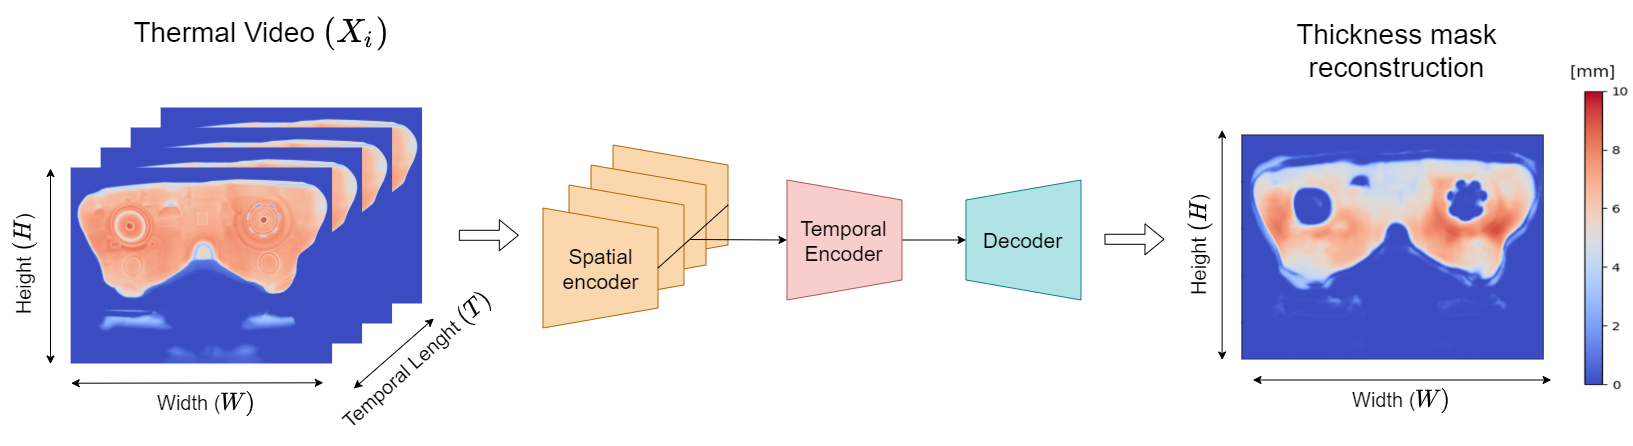
\includegraphics[scale=0.35]{images/chapter_4/Spatio-Temporal.png}
\caption{Spatio-temporal architecture}
\label{fig:spatio_temporal_architecture}
\end{sidewaysfigure}
%
The proposed pipeline is largely inspired by the \textit{Unet} (see Section \ref{U-Net}), and consists of three main blocks: the spatial encoder, the temporal encoder and the spatial decoder. 

\begin{itemize}
    \item \textit{Spatial Encoder:} The spatial encoder is a CNN which aims to extract the spatial feature map for each frame of the video. 
    We use the encoder of a traditional encoder-decoder architecture. Compared to the original \textit{Unet} architecture, we replace the original contracting path proposed in the paper with a Residual Network (ResNet, see Section \ref{Residual Networks}). The ResNet architecture is composed of five main building blocks. Each block sequentially produces higher-level and lower-resolution features which will later be used by the decoder to predict thicknesses. The general input thermal video is a four-dimensional tensor of shape $(h, w, c, t)$ where $h$, $w$, $c$ and $t$ are respectively the height of the image, the width, the number of channels and the number of frames of the video sequence. The spatial encoder processes each frame $(h, w, c)$ of the input thermal video and returns a feature map of size $(h', w', c', t)$ where $h'<<h$, $w'<<w$ and $c'>>c$ and a set of intermediate feature maps.
    

    \item \textit{Temporal Encoder:} The temporal encoder aims to encode the temporal information of the spatial feature maps produced by the spatial encoder, which encodes each frame independently, without leveraging any kind of temporal information. In order to process the temporal information, we use a 3D convolutional layer with a kernel size of $(1\times1\times1)$, stacked right after the spatial encoder, which produces a linear projection of the stack of frame-wise feature maps. This projection acts as a dimensional reduction along the temporal axis. In such a way we are able to produce a new feature map which encodes both the spatial and the temporal information. Given the spatial feature map of size $(h', w', c', t)$, the temporal decoder compress the temporal dimension and produces a new \textit{spatio-temporal feature map} with size $(h', w', c', 1)$.  The same convolutional operation, with the same parameters, is applied to compress the temporal information of all the intermediate features maps produced by the spatial encoder.
    
    \item \textit{Decoder:} The decoder projects the discriminant spatio-temporal feature map back to the original input spatial dimension. In the same way as for the \textit{Unet} architecture, intermediate high-level low-resolution features from the encoder path are combined and reused with the upsampled output of each decoder block to help the model reconstructing the prediction mask. The decoder is composed on five decoder blocks and each decoder block applies an upsample operation using the nearest neighbour algorithm followed by two 2D convolutional layers with a kernel size of $3\times 3$, batch normalisation and \textit{ReLu} activation function. A final convolutional layer produces the thickness map from which the prediction of the thickness of the critical  points is extracted. Given the encoded pattern of size $(h', w', c', 1)$ the decoder projects the encoded pattern to the original spatial dimension producing a 1-channel map reconstruction $(h, w, 1)$. Given the pixel coordinates of the $n$ critical points, their corresponding thickness predictions can be easily retrieved.
\end{itemize}

Training such an architecture is more challenging compared to that of the flexible temporal approach because of the number of learnable parameters. Furthermore, we have two main shortcomings:

\begin{itemize}
    \item The size of the training sample is low compared to what is normally used to train this kind of network. For semantic segmentation tasks, a dataset of 1000 images is considered small and we could hardly have more than a few hundred input samples.
    \item The thickness ground-truth map is not known for all the points of the tanks. In the training phase, semantic segmentation requires the output mask of the input data. For our problem, we do not have access to the full thickness map of the tanks, but only to the thickness of key points.
\end{itemize}

The first shortcoming may be alleviated by applying two different machine learning techniques: \textit{transfer learning} (see Section \ref{Transfer Learning}) and \textit{data augmentation}. Instead of training a model from scratch, a network with pre-trained parameters may be used as a starting point. Most of the state-of-the-art semantic segmentation approaches make use of pre-trained encoders to start with, while the remaining part of the network is trained from scratch. However, we deal with thermal images. Unlike traditional colour images, which are commonly represented using a 3-channel matrix (\textit{RGB}) with 256 different integer values, thermal images are 1-channel matrices where each pixel takes a continuous value corresponding to a temperature in degrees Celsius. Because pre-trained networks have been trained on RGB images composed of unsigned integers ranging from 0 to 255, to leverage transfer learning is necessary to map the continuous temperatures values to the 0-255 range. 

Data augmentation is a second option to deal with small datasets. Data augmentation in data analysis is a set of techniques used to increase the amount of data by adding slightly modified copies of already existing data or newly created synthetic data from existing data. Popular image augmentation techniques involves geometric transformations such as image flipping, rotation or translation, or colour space transformations. More advanced techniques make use of generative models to create artificial training sample. Regarding our problem, the only augmentation techniques that can be readily applied are the ones that involve geometric transformations. 
\begin{figure}
\centering
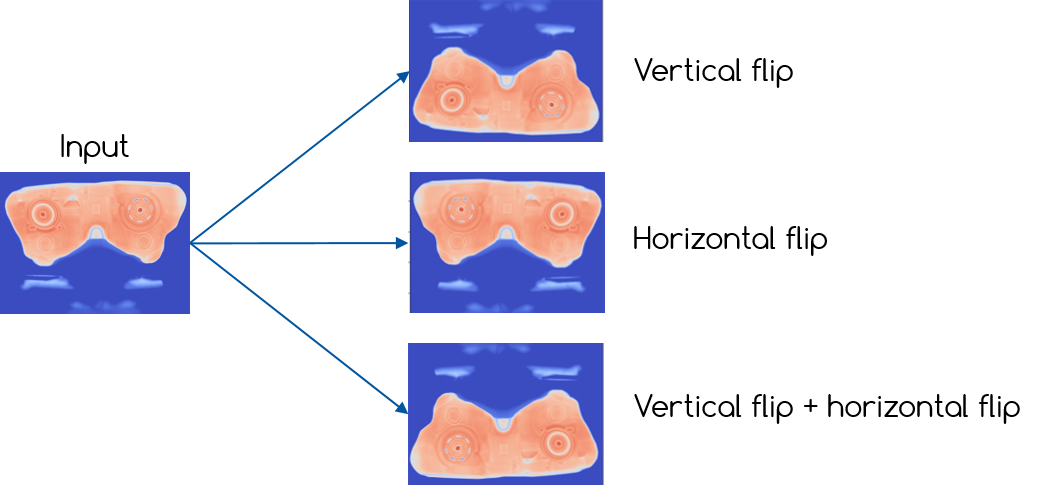
\includegraphics[scale=0.8]{images/chapter_4/data_augmentation.png}
\caption{Image augmentation}
\label{fig:image_augmentation}
\end{figure}

As image colour is temperature related, any augmentation techniques that alter the colour space risk corrupting the input data.
While the lack of a large volume of input data can be handled by transfer learning and data augmentation, the lack of labelled data in the training dataset can be a little more challenging. In fact, since the full thickness map of the part is not available, we cannot train the model in the traditional pixel-wise loss between the ground truth map and its reconstruction computed by the network. The computed loss is then back-propagated in the network to adjust the learnable parameters of the architecture. In our particular case, the full thickness ground truth of the part is not known, which means that we cannot compute the pixel-wise loss everywhere. However, it is possible to train the network by computing the pixel-wise loss between the map and the reconstruction for the pixels whose thickness is known.

\section{Experimental validation} \label{Experimental Validation}

This section presents the results from a real-world implementation in an industrial setting. First, the empirical context is described as well as the data processing and the training pipeline. Finally, we provide the results of this first experimentation.

\subsection{Data collection}

To evaluate the performance of the proposed data-driven model-based quality control, a data acquisition campaign in an industrial environment has been organised. In order to train our models to learn to infer the thickness, given the cooling profile, we need two different types of data: the temperature of the part surface and the thickness measurement of the corresponding part. The temperature data  has been acquired with an industrial thermal camera OPTRIS PI 640 with a good resolution (640$\times$480), previously calibrated to correctly measure the temperature of the plastic material. Unlike traditional colour images, which are commonly represented using a 3-channel matrix (\textit{RGB}) with 256 different integer values, thermal images collected through the OPTRIS 640 PI are 1-channel matrices where each pixel takes a continuous value corresponding to a temperature in degrees Celsius. Unlike other temperature measuring instruments, the thermal camera has the advantage to evaluate, in a single shot, the temperature of the whole visible surface. Several consecutive shots of the same part make it possible to follow the evolution of the temperature over time (Figure \ref{fig:thermal_video}). 

\begin{figure}
\centering
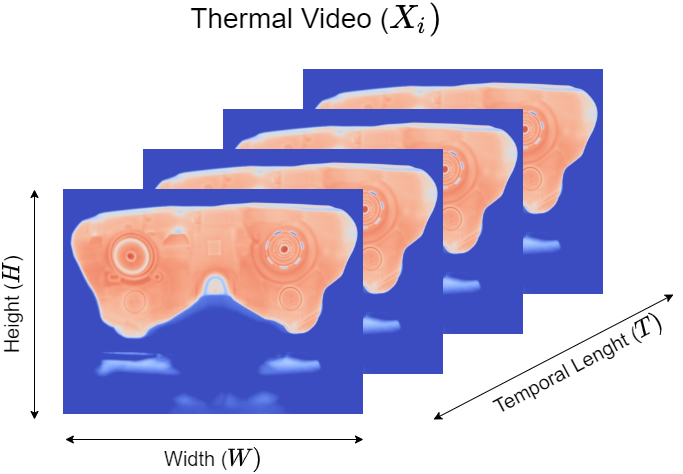
\includegraphics[scale=0.55]{images/chapter_4/Thermal_video.png}
\caption{Thermal video $X_i$}
\label{fig:thermal_video}
\end{figure}
%
In order to gather comparable data, the image acquisition of each part produced needs to be synchronised with the blowing process in order to synchronise the acquisition of images on the same relative time. Repeatable mechanical movements of the machine have been used to “trigger” data acquisition. The trigger starts a one minute countdown after which the acquisition of thermal images begins. This time is mandatory to give the machine the time to unload the part and the machine operator time to place the part in the measuring area. For our experimental measurement campaign, we collected thermal videos on 50 different parts. For each part we recorded 120 consecutive thermal images equally spaced with a one second interval between images, for a total of two minutes of data acquisition.

The thickness measurement has been carried out on key points through the use of an ultrasonic measurement instrument routinely used for sampling control. The thicknesses of the part selected for our experimentation have typical values ranging between 3 and 10 millimetres. For each thermal video, and therefore for each part, we measured 20 critical thickness points evenly distributed on the tank surface (Figure \ref{fig:critical_points}).

\begin{figure}
\centering
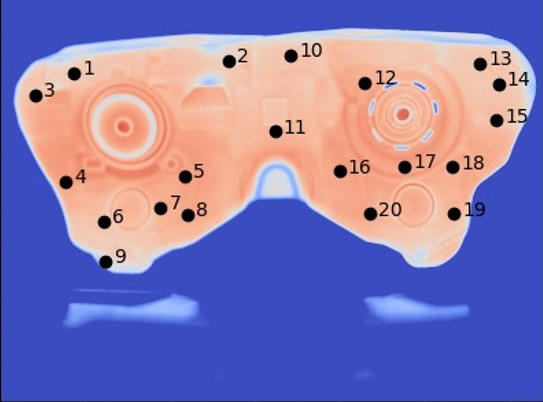
\includegraphics[scale=1]{images/chapter_4/critical_points.jpg}
\caption{Critical points distribution on the tank surface}
\label{fig:critical_points}
\end{figure}

\subsection{Data processing}

Once data have been collected, some processing operations are needed to prepare the data for training. Raw thermal frames are transformed in RGB images using a colormap which maps low temperature value to blue colours and high temperature value to red colours. In order to have comparable colours among the different frames, the colormap is computed on values ranging from 40\degree C (dark blue) and 135\degree C (bright red). Moreover, we need to associate the 20 key points whose thickness is measured to their corresponding pixel coordinates on the thermal video. This was done manually, each measured point of the part is identified on a thermal image by its $(\xi_{k}, \zeta_{k})$ pixel coordinate. Hopefully, since the position of the part does not change during the image acquisition, it is sufficient to find the pixel coordinates for one frame per sequence. 

Although the part does not move during the acquisition, each part is not precisely positioned with respect to the field of view of the thermal camera. The  $(\xi_{k}, \zeta_{k})$ coordinates on different thermal videos may therefore refer to different surface areas of the part. In order to align pixel coordinates along parts, a transformation is applied, to each frame, to project the part onto a reference position. Before describing the transformation in more detail, we present the \textit{pinhole camera model}. 

\paragraph{The pinhole camera model}
The pinhole camera model describes the mathematical relationship between the coordinates of a point in a three-dimensional space and its projection onto a two-dimensional pixel coordinate system. This mathematical relationship depends on the extrinsic and intrinsic parameters of the camera. The extrinsic parameters refer to the rotation matrix and translation vector of the camera coordinate system with regard to the world coordinate system.
Given a point $(x, y, z, 1)^{T}$ in the world coordinate system, we can form its pixel coordinates $(\xi, \zeta, 1)^{T}$ as follows:
\begin{equation} \label{pinhole}
    \begin{bmatrix} \xi\\ \zeta\\ 1 \end{bmatrix} = \begin{bmatrix}
        f_x & 0   & c_x\\ 
        0   & f_y & c_y \\ 
        0   & 0   & 1 
        \end{bmatrix}
        \begin{bmatrix}
        r_{11}& r_{12} & r_{13} & t_{x} \\ 
        r_{21}& r_{22} & r_{23} & t_{y} \\
        r_{31}& r_{32} & r_{33} & t_{z}
        \end{bmatrix}
        \begin{bmatrix} x\\ y\\ z \\ 1 \end{bmatrix}
        \enspace,
\end{equation}
That is:
\begin{equation}
    \begin{bmatrix} \xi\\ \zeta\\ 1 \end{bmatrix} = K[R|T]
    \begin{bmatrix} x\\ y\\ z \\ 1 \end{bmatrix}
        \enspace,
\end{equation}

where:
\begin{itemize}
    \item $K$ is the 3 $\times$ 3 intrinsic camera matrix.
    \item $f$ is the focal length.
    \item $(c_x,c_y)$ are the coordinates of the principal point at the center of the image plane.
    \item $R$ is the 3 $\times$ 3 rotation matrix.
    \item $T$ is the translation vector.
    
\end{itemize}

Given this  mathematical description, a homography $H$ can be defined as a transformation matrix that maps points from one plane to another. It can be derived by the equation \ref{pinhole}:

\begin{equation}
    \begin{bmatrix} \xi\\ \zeta\\ 1 \end{bmatrix} = \begin{bmatrix}
        f_x & 0   & c_x\\ 
        0   & f_y & c_y \\ 
        0   & 0   & 1 
        \end{bmatrix}
        \begin{bmatrix}
        r_{11}& r_{12} & r_{13} & t_{x} \\ 
        r_{21}& r_{22} & r_{23} & t_{y} \\
        r_{31}& r_{32} & r_{33} & t_{z}
        \end{bmatrix}
        \begin{bmatrix} \xi'\\ \zeta'\\ 0 \\ 1 \end{bmatrix}
\end{equation}

\begin{equation}
    \begin{bmatrix} \xi\\ \zeta\\ 1 \end{bmatrix} = \begin{bmatrix}
        f_x & 0   & c_x\\ 
        0   & f_y & c_y \\ 
        0   & 0   & 1 
        \end{bmatrix}
        \begin{bmatrix}
        r_{11}& r_{12} & t_{x} \\ 
        r_{21}& r_{22} & t_{y} \\
        r_{31}& r_{32} & t_{z}
        \end{bmatrix}
        \begin{bmatrix} \xi'\\ \zeta'\\ 1 \end{bmatrix}
\end{equation}

\begin{equation}
    \begin{bmatrix} \xi\\ \zeta\\ 1 \end{bmatrix} = 
        \begin{bmatrix}
        h_{11}& h_{12} & h_{13} \\ 
        h_{21}& h_{22} & h_{23} \\
        h_{31}& h_{32} & h_{33}
        \end{bmatrix}
        \begin{bmatrix} \xi'\\ \zeta'\\ 1 \end{bmatrix}
\end{equation}

\begin{equation} \label{projection}
P=HP'
\end{equation}

where:

\begin{itemize}
    \item $P$ and $P'$ are two points on different planes.
    \item $H$ is a 3 $\times$ 3 matrix composed by intrinsic and extrinsic parameters that relate the two planes together.
\end{itemize}


The mathematical framework presented above can be applied to project all the thermal frames composing the 50 thermal video collected over a reference image. By estimating the homography between the two planes, that of the reference image and that of the image to be projected, each point $P$ of the input image can be projected to the reference image. 

The first frame of each thermal video sequence is used to estimate the homography matrix, through the use of the ORB (Oriented FAST and Rotated BRIEF) algorithm \citep{rublee2011orb}. In a nutshell, ORB is a feature matching algorithm that allows to automatically find some key points in an image. The ORB algorithm takes as inputs two images, a reference and the one we want to project on this reference, and features that can be matched in the two images are used to estimate the homography matrix. Once the homography is computed, it is applied to map all the pixels of the second image to the pixel of the reference image. The same transformation can then be applied to all the frames in the video sequence, provided that both the camera and the tank are motionless. 
%
Then, depending on the used method, extra processing is needed to prepare data for training.

\subsubsection{Parametric temporal approach}
The parametric temporal approach makes use of the temperature time series extracted from the thermal video sequences to infer the corresponding thickness. Given the coordinates $(\xi_{k}, \zeta_{k})$ of the 20 critical thickness values, it is simple to retrieve the temperature time series by simply collecting the temperature of the coordinate for each sequential frame of the thermal video. By extracting all temperature time series for each critical point of the 50 parts considered, we can build a new time series dataset composed of 1000 (50 x 20) time series and the corresponding thickness values. The time series are then approximated by their parametric expansion. As explained in Section \ref{Parametric Temporal approach}, three different parametric functions have been identified as good candidates for approximating the pixel-wise temperature surface decay. In order to identify the parametric expansion that best fits the input time series, each expansion was applied to the time-series of the training set. The root mean square error (RMSE) of the overall reconstruction is used to select the best expansion. 

Table \ref{tab:curve_fitting_error} shows the average RMSE reconstruction for the three parametric expansions considered. The polynomial expansion, minimises the reconstruction error and is thus used to summarise the raw time series.  
For each time series, the three parameters defining the second-order polynomial approximation constitute the predictor of the machine learning model.

\begin{table}
\centering
\caption{Curve fitting reconstruction error}
\begin{tabular}{ll}
\toprule
\textbf{Parametric function}    & \textbf{RMSE (train)}\\ 
\midrule

Power Law              & 0.29         \\ 
Logarithmic            & 0.27         \\ 
Polynomial (2nd degree) & 0.03         \\ 
\bottomrule
\end{tabular}
\label{tab:curve_fitting_error}
\end{table}


\subsubsection{Flexible temporal approach}

As for the parametric temporal approach, the flexible temporal approach makes use of the temperature time series extracted from the thermal video sequences to infer the corresponding thickness. Given the coordinates $(\xi_{k}, \zeta_{k})$ of the 20 critical thickness values, it is simple to retrieve the temperature time series by simply collecting the temperature of the coordinate for each sequential frame of the thermal video. Unlike the previous approach, no extra data processing is required because the raw time series constitute the input data of the RNN model. 

\subsubsection{Spatio-temporal approach}
Compared to the previous approaches, the spatio-temporal approach does not require to rearrange the input thermal video in another format, but some processing operations are still needed to allow the usage of a pre-trained spatial encoder. In order to be consistent with the data of the \textit{ImageNet} dataset \citep{deng2009imagenet} that was used  to pre-train the network, each thermal frame is converted to a 3-channel RGB image. The maximum and minimum temperatures among all frames are retrieved and the same colormap is applied on all thermal frames of each video sequence. The colormap is the one applied to visualise the thermal frames in the current Chapter. All values are then rescaled in $[0, 1]$ and then normalised using the default mean and standard deviation value of the \textit{ImageNet} dataset.

\subsection{Training}

In this section our training pipeline is presented. For each approach, the data was divided into three sets: the training set (data from 38 parts), the validation set (data from 8 parts) and the test set (data from 5 parts). The training is used to fit the models, the validation set is used to select the model hyper-parameters and the test set is used to evaluate the ability of the model to generalise on new data. For each proposed approach, a Bayesian optimization of hyper-parameters with the \textit{Tree-structured Parzen Estimator} (TPE) \citep{bergstra2011algorithms} algorithm was used to select the hyper-parameters that minimise the \textit{Mean Squared Error} (MSE) on the validation set.

\subsubsection{Parametric temporal approach}

As explained previously, a second-degree polynomial is fitted over the time series to compress the input data into a few features corresponding to the coefficients of the polynomial expansion of the thermal signal. Three machine learning algorithms were compared to model the relationship between the polynomial coefficients and the corresponding thickness values: \textit{Lasso} (linear) regression, \textit{random forest} and \textit{Support Vector Machine} (linear or kernelised) regression. 
The exhaustive list of model hyper-parameters and their search space is summarised in Table \ref{tab:Parametric Temporal_search_space}.

\begin{table}
\centering
\caption{Hyper-parameter search space for the parametric temporal models}
\label{tab:Parametric Temporal_search_space}
\begin{tabular}{@{}l@{~\,}ll@{}} 
\toprule
\textbf{Model}                            & \textbf{Hyper-parameter} & \textbf{Search space}                          \\ 
\midrule
Lasso                                     & $\lambda$                & LogSpace($10^{-5}$, 1)                          \\ 
\midrule
\multirow{4}{*}{SVM}  & Kernel                   & \{Linear, Polynomial, RBF\}  \\ 
\cline{2-3}
                                          & $C$                        & LogSpace($10^{-6}$, 1)                          \\ 
\cline{2-3}
                                          & Polynomial degree (Polynomial) & [2, 4] \\
\cline{2-3}
                                          & $\gamma$ (\{Polynomial, RBF\}) & LogSpace($10^{-3}$, $10^{3}$) \\
                                          
\midrule
\multirow{3}{*}{Random Forest}  & Number of predictors     & [50, 500]                       \\ 
\cline{2-3}
                                          & Maximum tree depth       & [4, 50]                           \\ 
\cline{2-3}
                                          & Minimum samples leaf     & [1,60]                           \\
\bottomrule
\end{tabular}
\end{table}

\subsubsection{Flexible temporal approach}
We compared the performances of three RNN-based models: a vanilla RNN, an LSTM and finally a GRU network. The number of hidden units of each computational cell, as well as the number of stacked layers are hyper-parameters that are optimised. A comprehensive summary of the search space for the hyper-parameters is available in Table \ref{tab:rnn_search_space}. 

\begin{table}
    \centering
    \caption{Hyper-parameter search space for the flexible temporal models}
    \begin{tabular}{ll}
    \toprule
    \textbf{Hyper-parameter} & \textbf{Search space} \\ 
    \midrule
    RNN Cell type & \{RNN, LSTM, GRU\} \\
    N\degree  hidden unit & \{8, 16, 32\} \\
    N\degree  stacked layers & \{1, 2\} \\
    \bottomrule
    \end{tabular}
    \label{tab:rnn_search_space}
\end{table}
Each model has been trained to minimise the mean squared error metric using the  \textit{Adam} optimiser~\citep{kingma2014adam} with $\beta_{1} = 0.9$, $\beta_{2} = 0.98$ and $\epsilon = 10^{-9}$ (default values) and a learning rate sampled by the TPE algorithm on a logarithmic scale,  from $10^{-7}$ to $10^{-2}$. 

\subsubsection{Spatio-temporal approach}
As for the previous approach, we compared different model configurations on two pre-trained networks: a ResNet18 (18 layers) and a ResNet34 (34 layers). Deeper architectures exist, but we made the choice to limit the search space to the two smaller ResNet architectures because of the limited number of samples in our training set. Deeper architectures would allow to extract richer data representations, but at the expense of more parameters and increased computation time. We believe that ResNet18 and ResNet34 are powerful enough to produce a relevant representation of thermal images. Another hyper-parameter of the presented architecture is the number of encoder/decoder blocks. As stated in Section \ref{Residual Networks}, all ResNet architectures, independently on their depths, have 5 main building blocks. Actually, it is possible to slightly change the architecture in order to stop the encoding computation before the last block. This allows to reduce the complexity of the architecture and thus prevent possible over-fitting problems. For instance, we could take into account only the first 3 convolutional building blocks of the ResNet in such a way that the output of the third convolutional building block would be the spatial feature map and the output of the first and second blocks would be the intermediate encoded features. Since the encoder and decoder are symmetrical, reducing the number of encoder blocks also implies a reduction in the number of decoder blocks.

\begin{table}[h!]
    \centering
    \caption{Hyper-parameter search space for the spatio-temporal models}
    \begin{tabular}{ll}
    \toprule
    \textbf{Hyper-parameter} & \textbf{Search space} \\ 
    \midrule
    Encoder & \{ResNet18, ResNet34\} \\
    N\degree  of blocks  & \{3, 4, 5\} \\
    \bottomrule
    \end{tabular}
    \label{tab:spatial_temporal_search_space}
\end{table}

As for the flexible temporal approach, each model configuration has been trained to minimise the MSE metric using \textit{Adam} optimiser with $\beta_{1} = 0.9$, $\beta_{2} = 0.98$ and $\epsilon = 10^{-9}$ and a learning rate sampled by the TPE algorithm on a logarithmic scale from $10^{-10}$ to $10^{-2}$. 

\subsection{Results}

In this section the results obtained with the three approaches are presented and compared. Performances are measured using the Root Mean Squared Error (RMSE), which has the benefit of penalising large errors and whose value is easy to interpret because it has the same unit as the dependent variable: all the scores presented below represent the average thickness reconstruction error in millimetres.

For the parametric temporal approach, random forest performs better in both fit on the training set and generalisation on the test set (Table \ref{tab:Parametric Temporal_model_results}).
%
\begin{table}[h]
    \centering
    \caption{RMSE for the parametric temporal models}
    \begin{tabular}{llll}
     \toprule
    \textbf{Model} & \textbf{Train}  & \textbf{Validation}  & \textbf{Test}  \\
    \midrule
    Lasso & {0.95} & {0.91} & {0.89} \\
    Support Vector Regressor & {0.80} & {0.73} & {0.76} \\
    Random Forest Regressor & {0.19} & {0.54} & {0.48} \\
    \bottomrule
    \end{tabular}
    \label{tab:Parametric Temporal_model_results}
\end{table}
%
The error is about 0.5 mm, which is not accurate enough from the industrial point of view. However, this first experiment allowed us to demonstrate that there is a relationship between the temperature evolution of a zone of the part and the corresponding thickness, as assumed in  Section \ref{Motivation}.

\begin{figure}
\centering
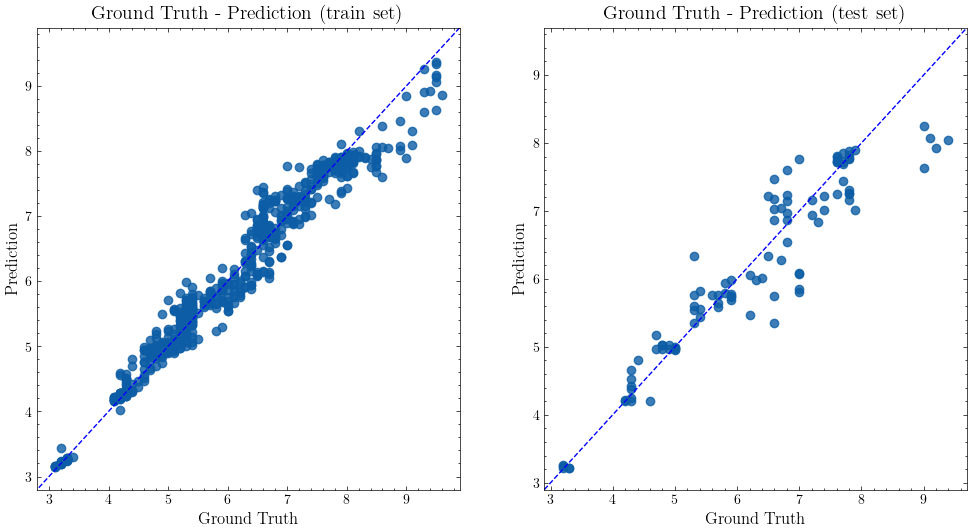
\includegraphics[scale=0.48]{images/chapter_4/temporal_scatter.png}
\caption{Prediction \textit{versus} ground truth scatter plots in train (left) and test (right) for the parametric temporal approach based on random forest regression}
\label{fig:gt_prediction_functional}
\end{figure}

Figure \ref{fig:gt_prediction_functional} shows the scatter plots of the predicted thickness and ground-truth thickness for the training and test sets. The plots confirm the ability of the model to distinguish between large and small thicknesses. Moreover, they show that the model is more accurate for thin points (close to 3 mm), which is positive because the thinnest points are also the most critical for the part to meet the customer's specifications.

Among all flexible temporal trained model, the configuration that minimises the validation error is a GRU model with 8 hidden units per cell and one layer. The results obtained are summarised in Table \ref{tab:temporal_model_results}.
%
\begin{table}
    \centering
    \caption{RMSE for the flexible temporal models}
    \begin{tabular}{llll}
    \toprule
    \textbf{Model} & \textbf{Train}  & \textbf{Validation}  & \textbf{Test}  \\
    \midrule
    RNN & {0.55} & {0.58} & {0.58} \\
    LSTM & {0.54} & {0.57} & {0.56} \\
    GRU & {0.54} & {0.56} & {0.54} \\
    
    \bottomrule
    \end{tabular}
    \label{tab:temporal_model_results}
\end{table}
%
These results are similar to those obtained with random forest, but random forest has a slightly lower error than GRU. Moreover, the computation time needed to train the random forest is significantly lower and it does not rely on dedicated hardware (GPU). The parametric temporal approach therefore seems preferable in all respects. This is confirmed in Figure~\ref{fig:gt_prediction_temporal}, where the parametric temporal approach outperforms the flexible temporal approach over all thickness ranges.
\begin{figure}
\centering
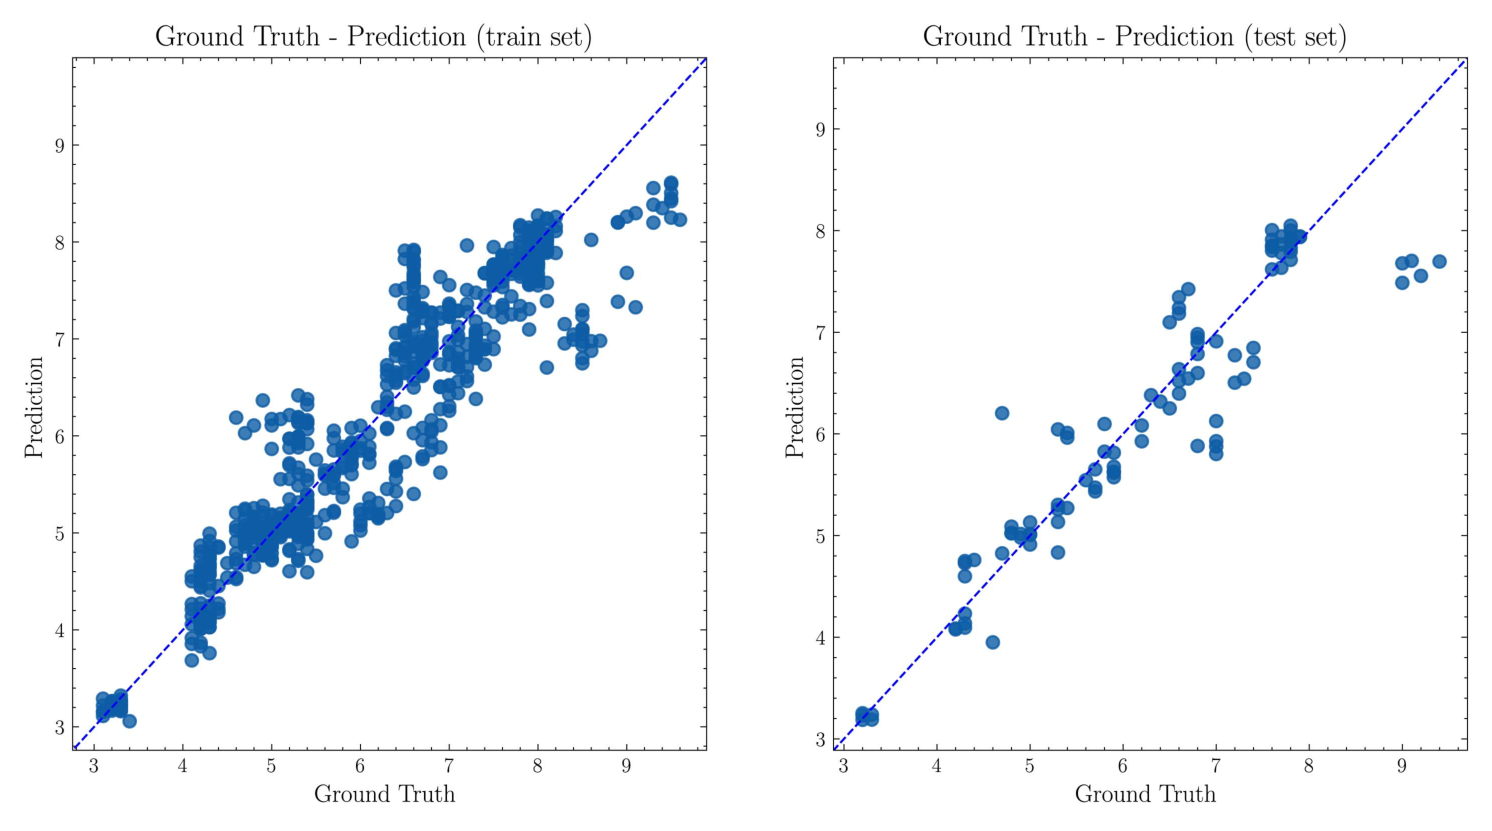
\includegraphics[scale=0.48]{images/chapter_4/gt_temporal.eps}
\caption{Prediction \textit{versus} ground truth scatter plots in train (left) and test (right) for the flexible temporal approach based on GRU}
\label{fig:gt_prediction_temporal}
\end{figure}

The third approach (Table \ref{tab:spatial_temporal_model_results}) completely outperforms the previous ones. The best results are obtained using a pre-trained ResNet34 encoder with 5 encoder-decoder blocks, which achieves an RMSE of 0.16 mm on the test set, which is about one-third of the error of the previous approaches. A precision of 0.2mm is considered extremely interesting in our industrial context. 
\begin{table}
    \centering
    \caption{RMSE for the spatio-temporal model}
    \begin{tabular}{llll}
    \toprule
    \textbf{Model} & \textbf{Train}  & \textbf{Validation}  & \textbf{Test}  \\
    \midrule
    ResNet34-5 blocks & \textbf{0.14} & \textbf{0.18} & \textbf{0.16} \\
    \bottomrule
    \end{tabular}
    \label{tab:spatial_temporal_model_results}
\end{table}
Figure~\ref{fig:gt_prediction_spatial_temporal} shows that the greatest benefits over the parametric temporal approach are at higher thicknesses, but the improvement is already visible at only 4 mm.

\begin{figure}
\centering
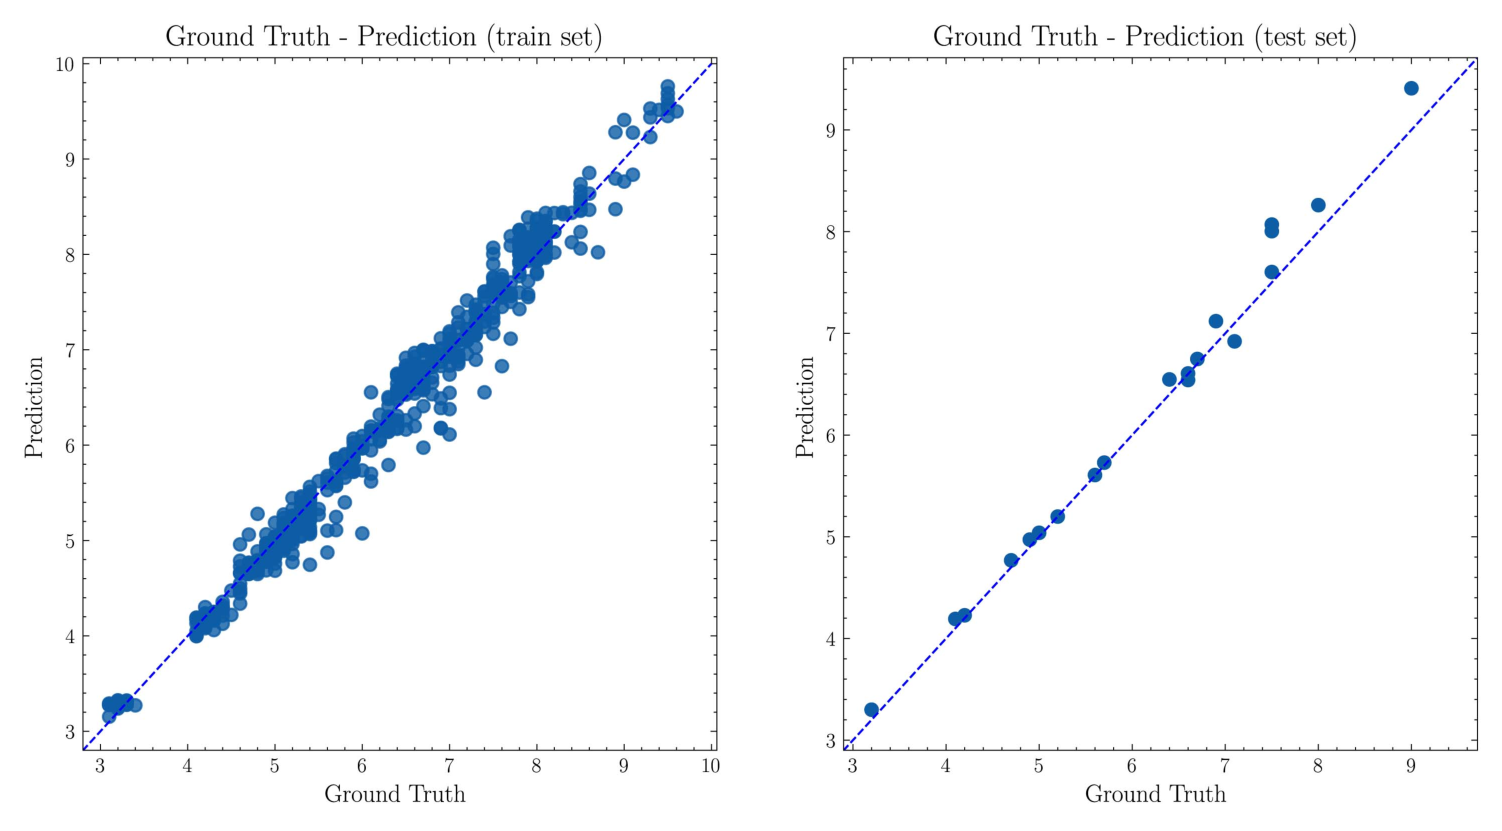
\includegraphics[scale=0.48]{images/chapter_4/gt_spatial_temporal.eps}
\caption{Prediction \textit{versus} ground truth scatter plots in train (left) and test (right) for the spatio-temporal approach based on ResNet34}
\label{fig:gt_prediction_spatial_temporal}
\end{figure}

\subsection{Model performance on unseen data point}

The results presented in the previous section show the ability of the spatio-temporal model to correctly estimate the thicknesses at the critical points of the part. The question is whether the model is able to generalise the relationship learned at a limited set of critical points to the entire surface of the part. The spatio-temporal architecture computes a thickness map for the entire surface of the tank. An example of the thickness map produced in this way is shown in Figure \ref{fig:thickness_mask_reconstruction} for a part in the test set. 
In this figure, the colour represents the predicted thickness, not the tank temperature.
The figure highlights the ability of the model to produce a thickness reconstruction beyond the critical points, but some areas, especially those close to the edge of the tank, are more difficult to predict. 
The prediction of thicknesses outside the critical points is unreliable.

\begin{figure}
\centering
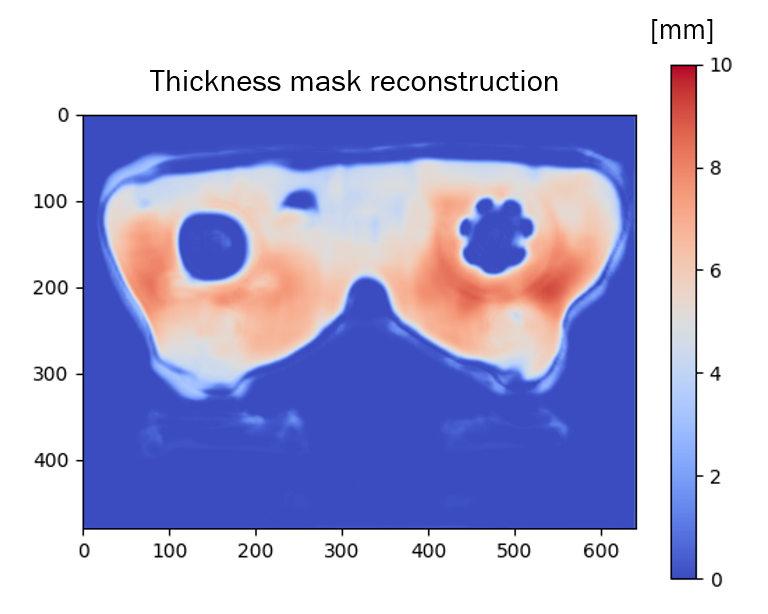
\includegraphics[scale=0.90]{images/chapter_4/mask_reconstruction.png}
\caption{Thickness mask reconstruction example}
\label{fig:thickness_mask_reconstruction}
\end{figure}

We modified the evaluation strategy to test accurately the accuracy of predictions outside of the measured critical points.
Since the entire thickness map is not available, we used only a subset of the 20 critical points to train the model, reserving the others to compute an out-of-critical-point prediction error. We removed 4 out of 20 critical points of the training set to adjust the model on the remaining points. The 4 points removed are then used to evaluate the ability of the model to predict the thickness outside critical points on test parts. This was repeated 20 times by randomly selecting the 4 removed points, to evaluate the results on a larger set, composed of $4\times20$ samples.
The results are presented in Figure \ref{fig:gt_prediction_unseen}, which shows a positive correlation between ground truth and prediction. 
%
\begin{figure}
\centering
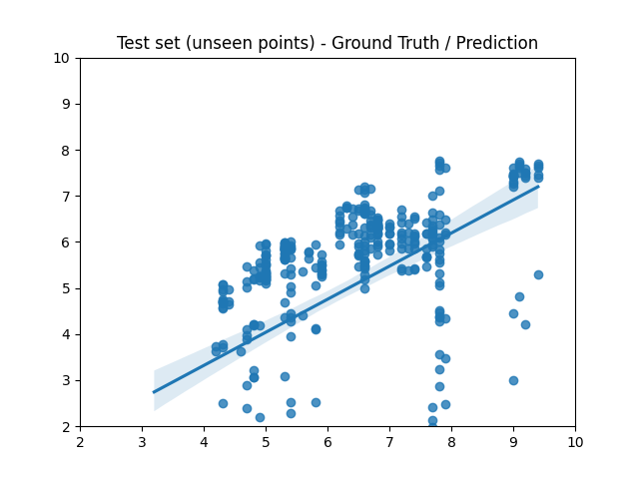
\includegraphics[scale=0.90]{images/chapter_4/unseen_point_scatter.png}
\caption{Prediction \textit{versus} ground truth scatter plot for the spatio-temporal approach based on ResNet34 on critical points not seen in training}
\label{fig:gt_prediction_unseen}
\end{figure}
%
However, the prediction of the thickness of unseen points is nowhere near as good as the prediction on these critical points, and our approach does improve on the manual inspection in this respect: our model is reliable on the critical points usually measured but fails to predict the thickness of the entire part.

\section{Conclusion}

Traditional quality control methods for measuring blow-moulded part thickness involves time-consuming operations that cannot be applied online for a 100\% quality inspection on all parts. This chapter proposes a new data-driven approach for measuring in real-time the part thickness by leveraging the surface-temperature decay over time. Three different pipelines have been designed to model the relationship between the cooling behaviour of a part area, captured through the use of a thermal camera, and the corresponding thickness. The procedure was validated in a real-world manufacturing setting. These results have shown the ability of our method to provide accurate results in predicting thickness values of a set of critical points. Among the three pipelines presented above, the spatio-temporal approach is the one that achieve the best performance in reconstructing the thickness values of the test set data. Future research works aim to generalise predictions outside of the critical points, in order to reconstruct the full thickness map of the whole visible part surface.

\subsection{Scientific contribution}

Thermography for measuring thickness is not a new idea, however, to our knowledge, this is the first time that thermography has been proven to be effective at measuring the thickness of a part in an industrial environment. Certainly the first time it has been used to infer the thickness of a blow-moulded part. By leveraging the surface-decay temperature due to the part cooling at the room temperature, we can infer the thickness of a tank in a non-contact manner.

Compared to previous proposed approaches using thermography, which make use of physics-based approaches to compute thickness given the surface decay temperature, we have decided to leverage the ability of data-drive methods to discover hidden patterns within data. The idea of using a data-driven approach is dictated by the following two motivations:

\begin{itemize}
    \item The tank is composed of multiple layers of different plastic material which complicates physical modelling. The physic model should take into consideration the different physical properties of each layer constituting the thickness of the fuel tank.
    \item The thermal inertia of the material, which causes an initial rise in temperature in the first few seconds after the tank has been blow-moulded, have to be taken into account. In our opinion, it is simpler to model this phenomenon through a data-driven approach. 
\end{itemize}

Transfer learning has been proven to be effective in a context where the number of data was very limited. Although the proposed method was validated in a single case study, we claim it should generalise to other industrial contexts. The presented empirical setting was designed to respond to a specific need of a manufacturer, but we think it should apply to others manufacturer dealing with blow-moulding and others manufacturing process involving plastic processing. Whenever it is possible to observe a different cooling behaviour between different areas of the part surface, our approach may be potentially applied.


\subsection{Industrial contribution}

From the industrial point of view, this chapter introduces a new idea of quality control. The traditional Acceptance Sampling approach, used in the industrial context studied, may be enhanced by introducing data-driven model quality control. In this chapter we have shown that by adding extra sensors, or cameras, it could be possible to infer the quality of the part and therefore provide a quality status in real-time without any time-consuming or destructive measurement. This provides to the manufacturing company a dual benefit:
%
\begin{itemize}
    \item It ensures a quality control on all parts produced which enable for a fast reaction to quality non-conformities. In fact, by ``virtually'' measuring each part, we are able to eventually discard parts for which the model has provided a ``Not-OK'' result, or request the quality team to carry out more in-depth tests. Model-based quality measurement may be effectively used to detect those parts that turn out to be, from a statistical point of view, outliers. In this way, instead of randomly sampling the parts to be measured by the quality operators, the model is able to suggest the parts that seem to be interesting. By discarding all non-compliant parts, this approach indirectly reduces product recalls and thus the whole series of requests to return, exchange or replace a product that has been found to be defective, and which could impair performance, harm consumers or cause legal problems for producers.
    \item Such an approach could be applied to reduce the real quality controls which destroy the parts or makes them unusable. In such a case, not only the data driven model-based control would be able to provide a thorough quality control, but it would also be able to reduce the scraps which account for an overall better production performance. Of course, real part measurements cannot be completely replaced by model-based measurements. In fact, real measurements are the primary data source for training the data-driven model. 
\end{itemize}
%
As regarding the proposed approach to infer the thickness, results are considered accurate enough to move towards the industrialisation of the proposed system. In order to industrialise the proposed system, we should be able to take into account extra information such us the temperature of the environment where the machine is located, as well as the temperature of the moulds. In fact, the surface temperature of the blow-moulded part depends on the ability of the moulds to absorb the heat. If the heat absorption capacity changes, as a result of the change in temperature of the moulds coolant, the tank surface temperature will be different and the data-driven model accuracy would drop. In the same way, the plant temperature may influence a bit the cooling behaviour of the blow-moulded part. However, the impact of the temperature of the industrial environment on the surface temperature decay should be minimal due to the insulating properties of the plastic material (PEHD).  

\cleardoublepage




\chapter*{Conclusion}
\addcontentsline{toc}{chapter}{Conclusion}
\thispagestyle{empty}

% TO BE MODIFIED
The future direction of Industrial Internet technology is to transform industrial processes and products, moving from the reliance on experience-based decision making towards data-centric or evidence-based decision making. It is through this process that Industrial AI will play a major role to advance the digitalization of traditional industrial systems.

\clearpage

\bibliographystyle{apalike}
\bibliography{references}
\addcontentsline{toc}{chapter}{Bibliography}

% Appendix
\appendix
% A
\chapter{Plastic Omnium}

Plastic Omnium is a French automotive supplier specialized in 
The company is composed of two divisions that are both leader in their field of activity:


\begin{figure}
\centerline{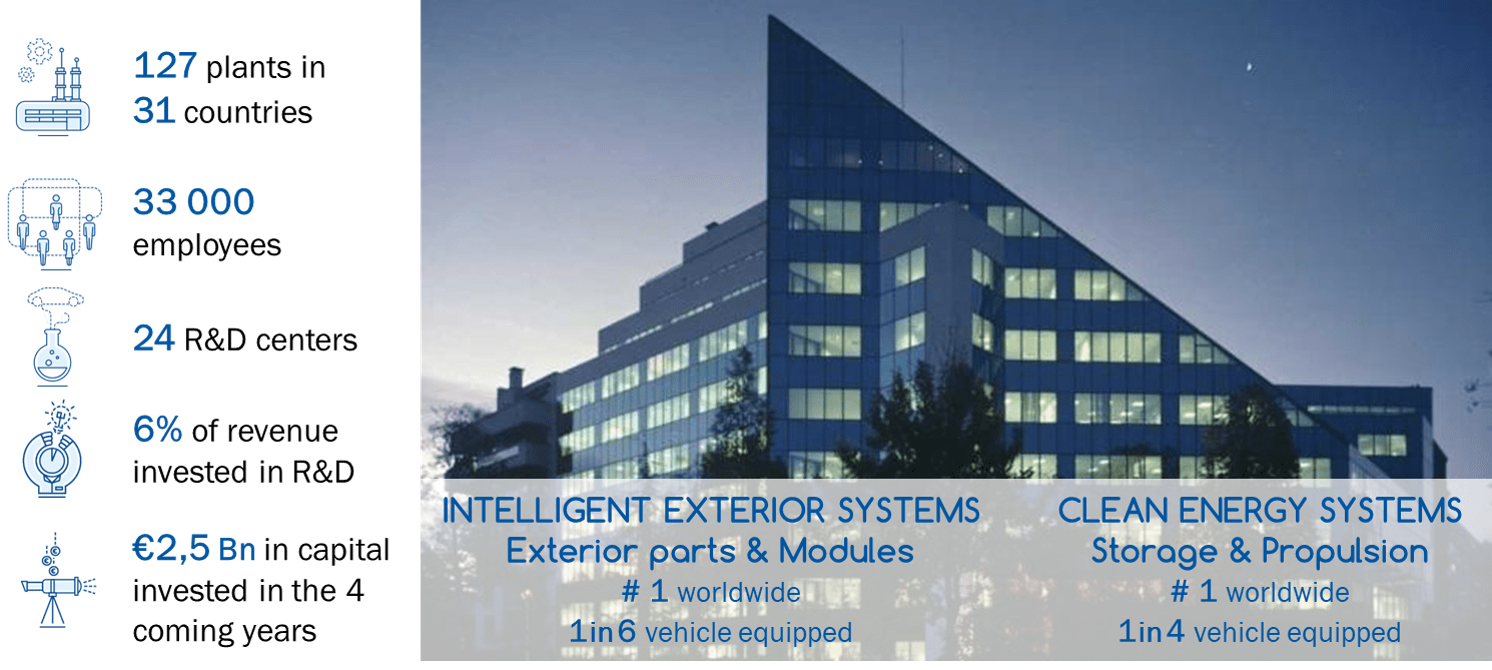
\includegraphics[scale=0.5]{images/appendix_A/PO_key_data.png}}
\caption{Plastic Omnium key data}
\label{fig:Plastic Omnium key data}
\end{figure}

%ADD image



\section{Clean Energy Systems}

The Clean Energy Systems (CES) division of Plastic Omnium is specialized in plastic fuel tanks systems, and depolluting systems, mostly for private and commercial vehicles. In 2018, more than 22M fuel systems have been delivered, representing 1 out of 4 commercialized vehicles equipped with a fuel system coming from the CES division.
The material used for producing the fuel tanks is HDPE (High-Density Polyethylene). There are several reasons why they are made of plastic and not in metal as they used to be (for cars):
\begin{itemize}
    \item Plastic is lighter than metal (about 30\%), which allows a reduction of fuel consumption.
    \item The raw material is less expensive.
    \item A plastic tank cannot explode: it will melt, and the fuel will be spilled on the floor.
\end{itemize}

However, one issue is the permeability: as plastic is a porous material, fuel will eventually end up going through it and that leads to two major issues: the consumer will lose some of his gas, and this one will go into the air and pollute the atmosphere. That is why a fuel tank is not a simple container of fuel: it’s a real part composed of complex technologies, from the production processes to the material used, and also the parts attached to the fuel system; filling system, pump gauge module, ventilation. These are used to make the fuel system (Figure \ref{fig:Fuel System}) less permeable to cope with the different regulations.
\begin{figure}
\centerline{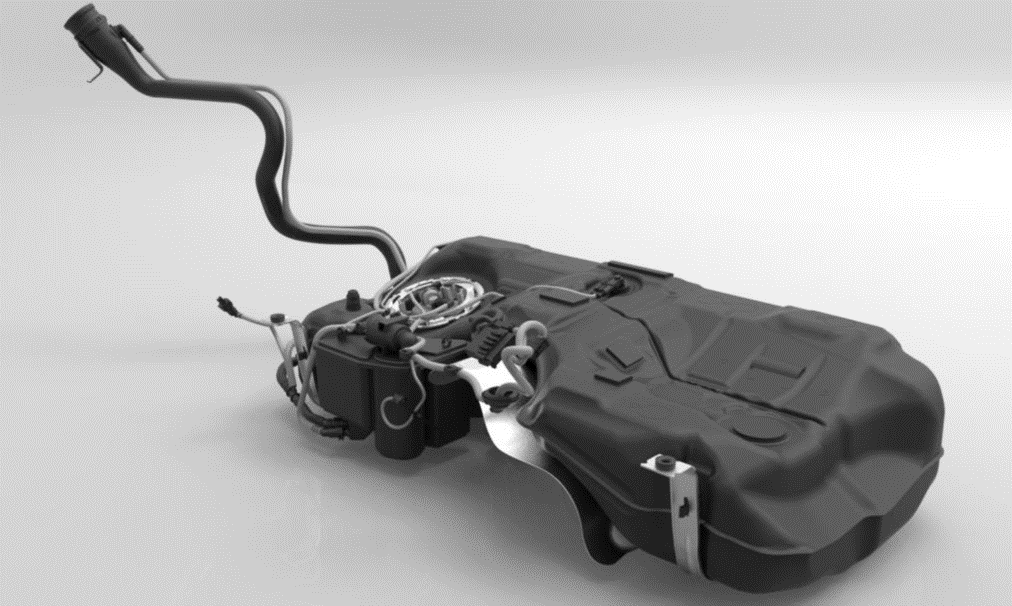
\includegraphics[scale=0.4]{images/appendix_A/fuel_system.png}}
\caption{Fuel System}
\label{fig:Fuel System}
\end{figure}
A fuel system is composed of a fuel tank (Figure \ref{fig:Plastic Fuel Tank}) and a filler pipe (Figure \ref{fig:Filler Pipe}, the latter is the only part visible of the system by the end user, to refill the tank at the station.

\begin{figure}
\centerline{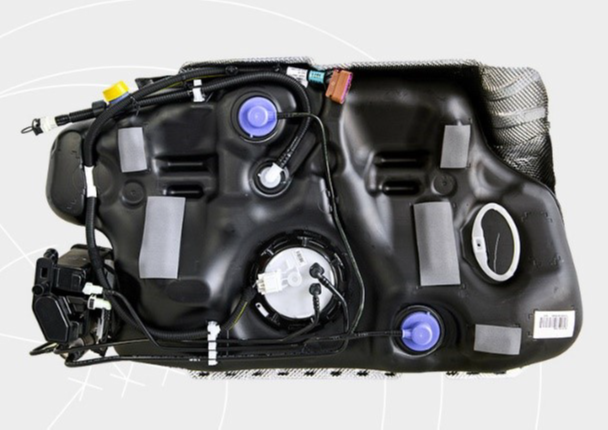
\includegraphics[scale=0.6]{images/appendix_A/Plastic_fuel_tank.png}}
\caption{Plastic Fuel Tank}
\label{fig:Plastic Fuel Tank}
\end{figure}
\begin{figure}
\centerline{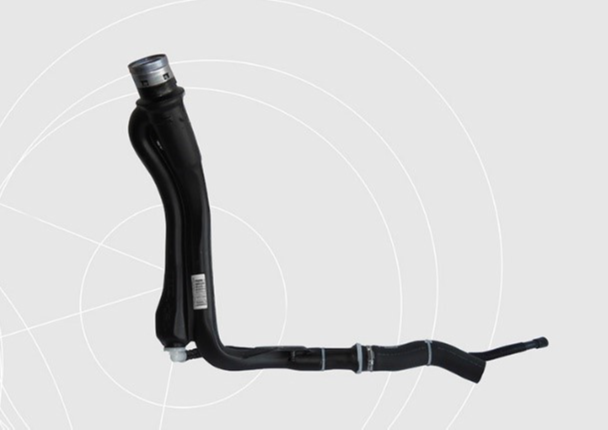
\includegraphics[scale=0.6]{images/appendix_A/Filler_pipe.png}}
\caption{Filler Pipe}
\label{fig:Filler Pipe}
\end{figure}

SCR technology is an effective response to the regulatory requirements limiting emissions of nitrogen oxides ($NO_x$) from diesel vehicles. Combining a tank with a pump and gauge module, this system injects vaporized \textit{AdBlue®} into the hot exhaust gases, causing a chemical reaction that transforms $NO_x$ into water vapor. Plastic Omnium has developed a range of SCR systems to meet the needs of all types of vehicles, from the smallest European city car to the largest American pickup truck.

\section{Intelligent Exterior Systems}

Intelligent Exterior Systems, IES, specializes in the manufacturing of complex car
body systems for car manufacturers. Examples of products are shown below: bumpers and
energy absorption systems, fender modules, front-end assemblies and rear-closure modules.

Today’s tailgate on boards state-of-the-art technology, customized and adapted to each customer requirements: plastic structure reinforced with metal or composite inserts, glued painted skin and local reinforcements to meet crash requirements.
Plastic Omnium designs also a range of exterior parts (fender flares, rocker panels, door trims) that add to the esthetic and distinctive character of the vehicles from each automaker.

\section{New Energies}

The \textit{New Energies} division, born in 2021, aims to contribute towards hydrogen-powered electric mobility. As part of the European H2HAUL project intended to deploy hydrogen mobility in road transport, the New Energy division has just produced vessels at its Herentals (Belgium) site. 

\begin{figure}
\centerline{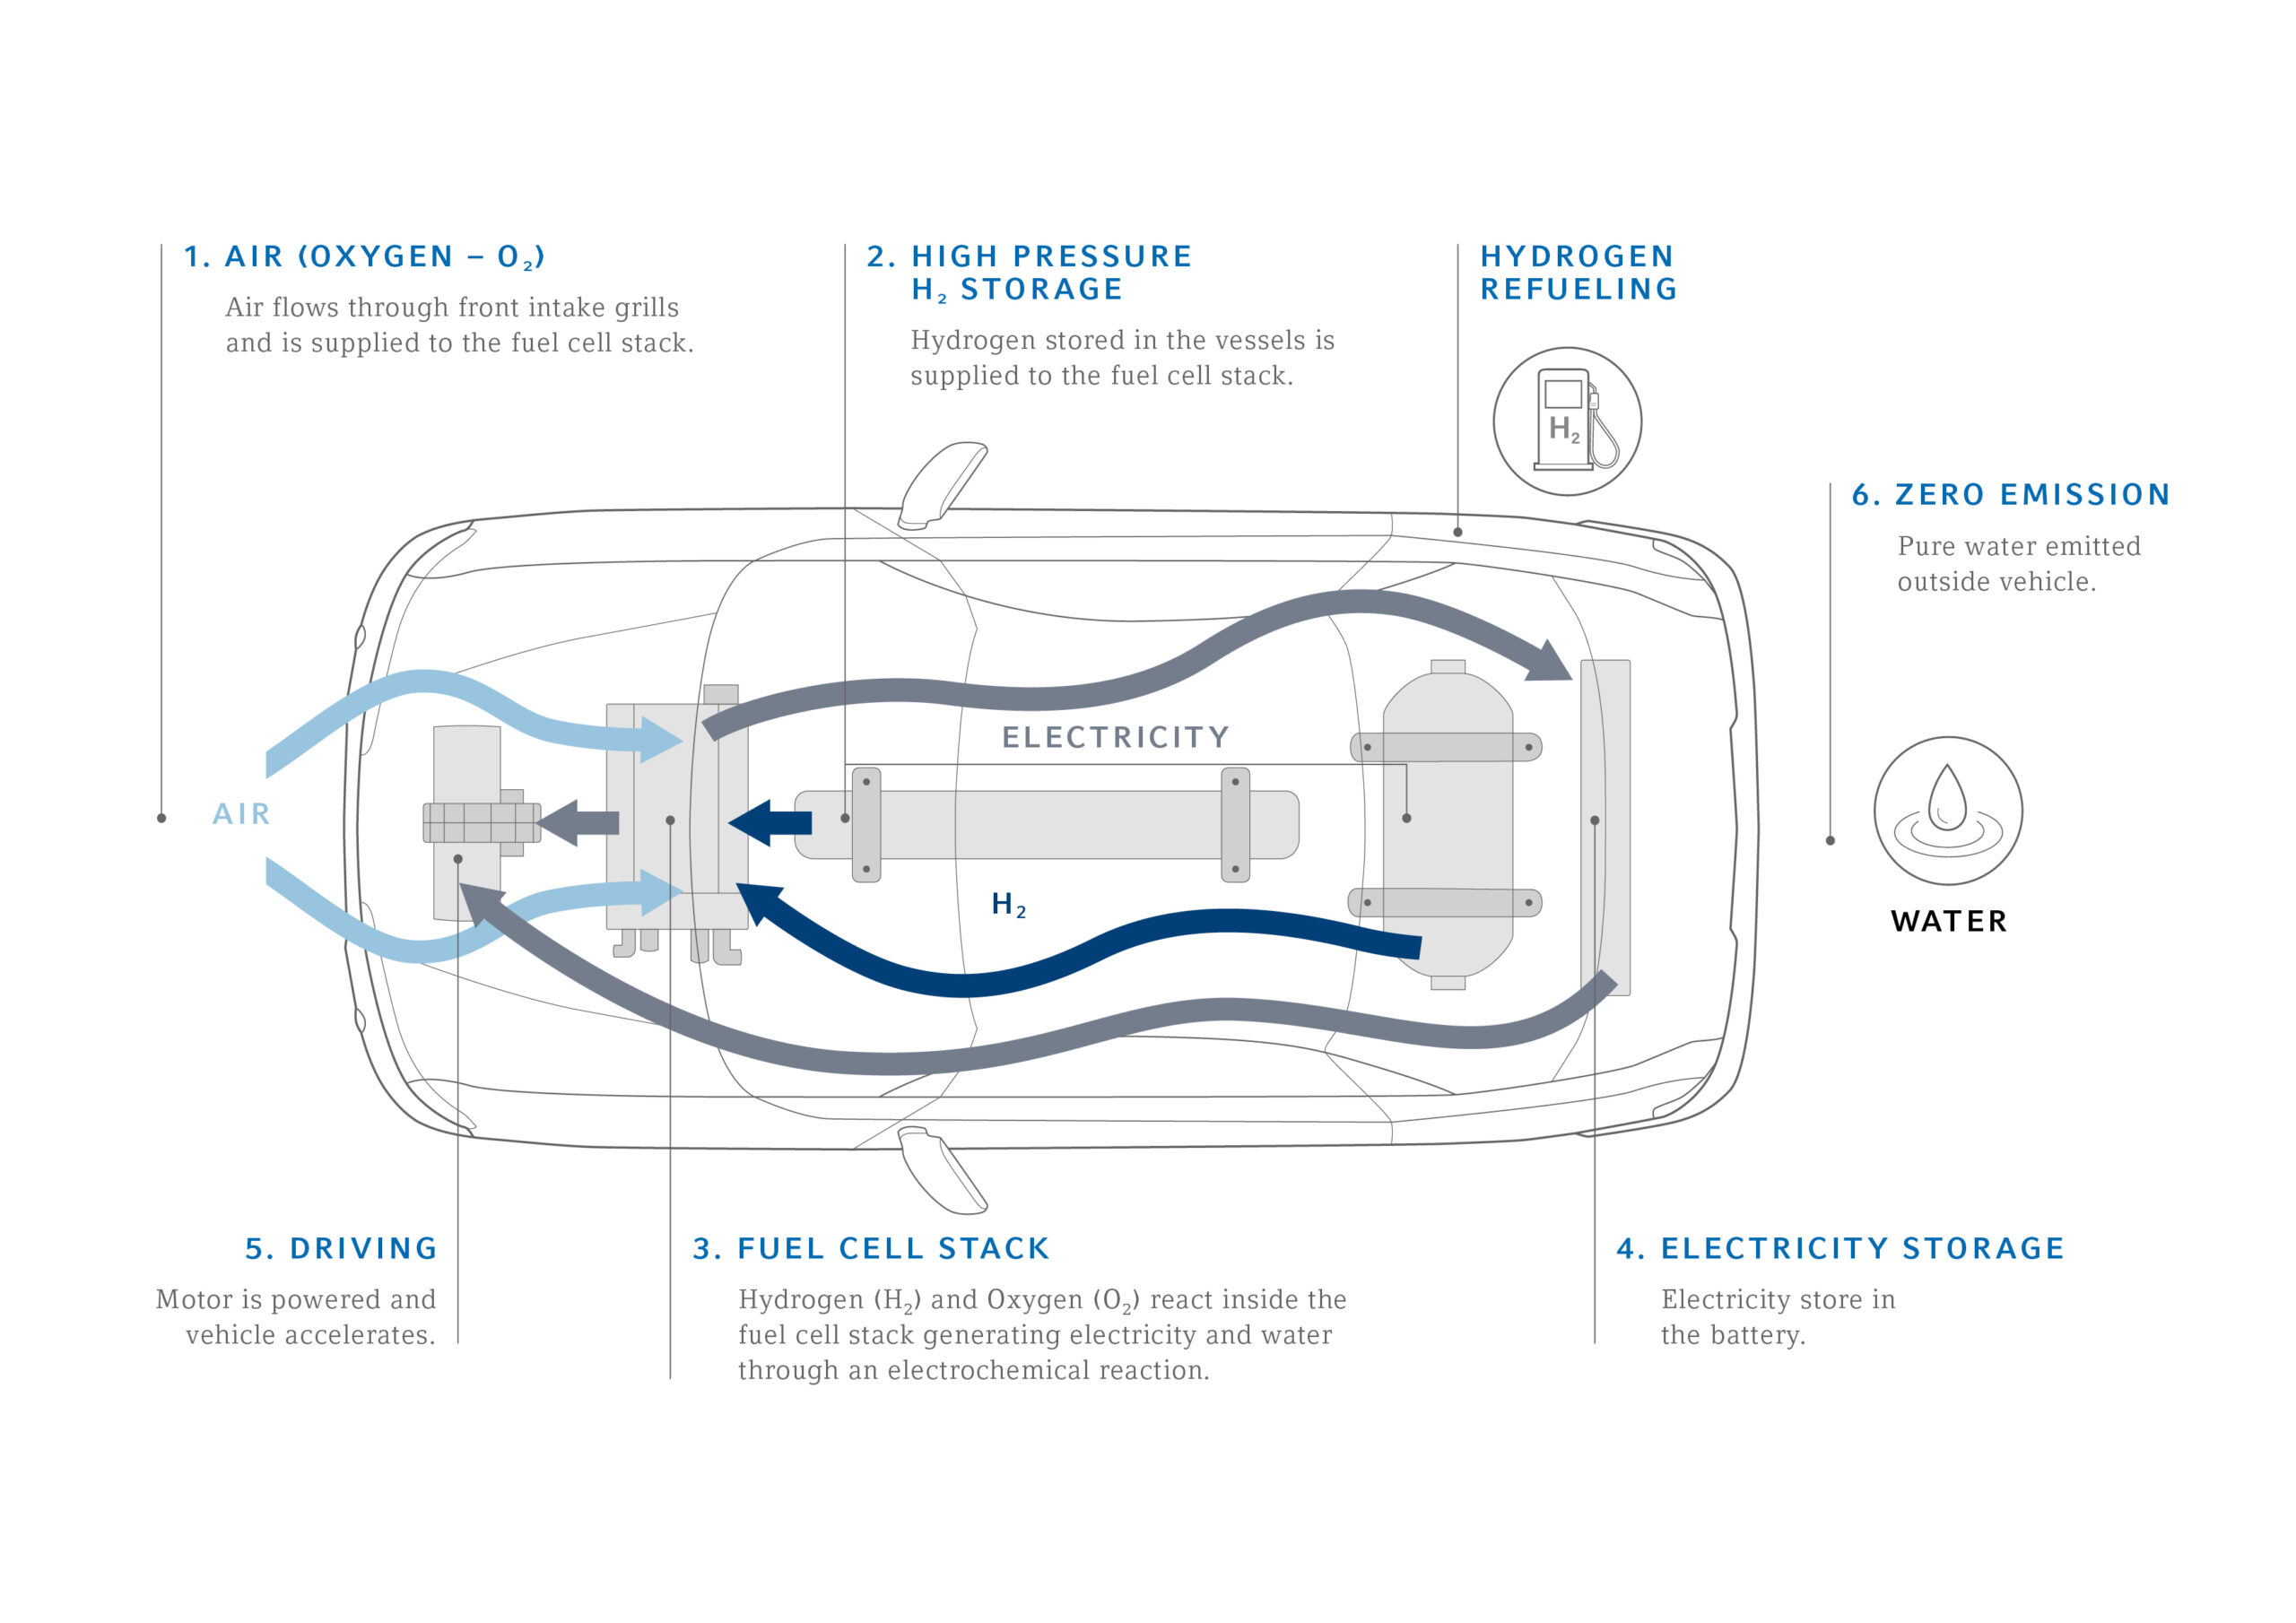
\includegraphics[scale=0.2]{images/appendix_A/plastic-omnium-voiture-zero-emission-legendes-scaled.jpg}}
\caption{Plastic Fuel Tank}
\label{fig:Plastic Fuel Tank}
\end{figure}

% B
\chapter{Full production process} \label{Full production process}

The industrial practice of producing a fuel tank part through the Extrusion Blow-Molding requires the following stages:

% Provide a two lines description
\begin{itemize}
    \item Material Supply: It constitutes all the equipment needed to provide the Extrusion Blow-Molding machine the raw material/s. 
    \item \textbf{Extrusion Blow-Molding}:
    \item Post Cooling; 
    \item Finishing: 
    \item Assembly:
\end{itemize}



Blow-molding is the first process to produce the fuel system. Once it has been blown, the flash around the tank is removed and regrinded, then it enters a phase of post-mold cooling, where its temperature is lowered with a water flow in a second mold. It is then stabilized in ambient air, before entering the finishing center, where parts of the tank will be cut, and extra components welded on it.
Then some parts will be assembled on the tank, such as the filler pipe presented above. Finally, every tank is tested to detect possible leaks.

The full process is detailed in Figure \ref{fig:Full_production_process}.

\begin{figure}
\centerline{\includegraphics[scale=0.4]{images/appendix_B/Blow_molding_process.png}}
\caption{Full production process}
\label{fig:Full_production_process}
\end{figure}

\end{document}
